%\documentclass{cumcmthesis}
\documentclass[withoutpreface,bwprint]{cumcmthesis} %去掉封面与编号页,电子版提交的时候使用。

\usepackage[framemethod=TikZ]{mdframed}
\usepackage{url}   % 网页链接
\usepackage{subcaption} % 子标题
\usepackage{algorithm}  
\usepackage{algpseudocode}  
\usepackage{amsmath}  
\usepackage{threeparttable} 
\renewcommand{\algorithmicrequire}{\textbf{Input:}}  
\renewcommand{\algorithmicensure}{\textbf{Output:}} 
\usepackage{ulem} 
\usepackage{setspace}
\usepackage{multirow}

\title{古代玻璃制品的成分分析与鉴别}


\begin{document}

 \maketitle
 \begin{abstract}


本文研究古代玻璃指标化学成分含量及类别的相关问题,建立偏最小二乘回归模型预测化学成分,利用改进的K-Means++聚类进行亚类划分,建立XGBoost多分类模型预测文物类别,并从宏微观的角度分析化学成分的关联关系。

\textbf{针对问题一},对于关系分析,利用\textbf{卡方独立性检验}对表面风化情况与三项特征变量的关联显著性进行分析,得到\textbf{玻璃类型}与有无风化的关联最显著。结合数据特征对该变量进行\textbf{降维}处理,最终得到\textbf{36种}特征组合并深入探讨。对于化学成分含量的统计规律分析,本文从描述性统计、数据分布规律、风化前后成分差异\textbf{三个维度}进行分析。其中,成分差异进行Mann-Whitney检验结合\textbf{机理分析},得出不同类型玻璃制品的主要影响成分。对于含量预测,本文结合化学成分含量的统计规律确定\textbf{基准化匹配策略},从而对风化与未风化数据进行\textbf{匹配}。以筛选所得主要影响成分作为重要变量建立\textbf{偏最小二乘回归模型}进行预测,得到风化前化学成分含量。


\textbf{针对问题二},首先对不同类型玻璃对应的化学成分含量差异进行\textbf{Mann-Whitney检验},得到具有显著差异的指标并进行\textbf{Logistic回归分析},得到玻璃类型的主要影响成分为\textbf{氧化铅}。对于亚类划分,利用\textbf{熵值法}与\textbf{均值乘数}得到量化权重,以此选取划分指标。之后,利用主成分分析法对所选指标进行\textbf{降维},并利用\textbf{量化权重}改进K-Means++算法,对数据进行聚类从而确定亚类划分。由此将铅钡玻璃划分为\textbf{4个}亚类,高钾玻璃划分为\textbf{3个}亚类。最终,本文利用\textbf{Kruskal-Wallis检验}以及亚类中表面有无风化的数据分布,分析亚类划分结果合理性,并调节量化权重进行敏感性分析。


\textbf{针对问题三},首先利用\textbf{氧化铅}对文物进行\textbf{基类划分},将文物初步分为铅钡玻璃与高钾玻璃。之后,利用回归方程将数据转化为风化前数据,并建立\textbf{XGBoost多分类模型}对玻璃文物的亚类进行预测。其中,本文利用\textbf{K折交叉验证}与\textbf{贝叶斯调参}对分类模型进行求解,预测所得F1分数为\textbf{0.826},效果较好。

\textbf{针对问题四},本文分别从宏观和微观层面对关联关系以及差异性进行分析。对于\textbf{宏观层面}分析,本文利用\textbf{Kendall's W检验}分析关联关系的显著性,利用\textbf{配对t检验}分析关联关系的差异性。对于\textbf{微观层面}分析,本文基于\textbf{改进熵权法}赋权,建立\textbf{灰色关联量化}模型,对化学成分间的关联关系及差异性进行量化分析。得到对于铅钡玻璃,与其他化学成分关联强度最大的化学成分为\textbf{氧化镁},对于高钾玻璃为\textbf{氧化钙}。\textbf{二氧化硅}与其他化学成分间的关联关系在不同种类的玻璃中体现出最大的差异性。

\textbf{本文的优势在于:}1.利用量化权重改进K-Means++算法,使聚类结果更加合理;2.从宏微观角度探讨化学成分的关联关系,使分析更完善全面。

\keywords{ 基准化匹配策略 \quad  偏最小二乘回归 \quad  K-Means++ \quad  XGBoost \quad 灰色关联量化}
\end{abstract}

\section{问题重述}

\subsection{问题背景}

近年来,在中国“一带一路”倡议的推动下,中外文化互学互鉴,互利共赢。“一带一路”倡议的核心在于“互联互通”,这也正是古代丝绸之路的要旨所在。丝绸之路是自古以来贯穿东西方的重要交流通道,而玻璃正是伴随着丝路上的商业贸易与文化交流传入我国的重要工艺品。

玻璃的主要原料是石英砂,在制作过程中还需添加助熔剂以降低熔化温度,不同的助熔剂常常会导致玻璃制品的主要化学成分不同。
在以铅矿石作为助熔剂时,烧制而成的玻璃制品为铅钡玻璃,而以草木灰作为助熔剂将会得到钾玻璃。此外,古代玻璃常受埋藏环境影响而发生风化,从而导致其成分比例发生变化,影响对其类别的正确判断。

\begin{figure}[H]
\centering
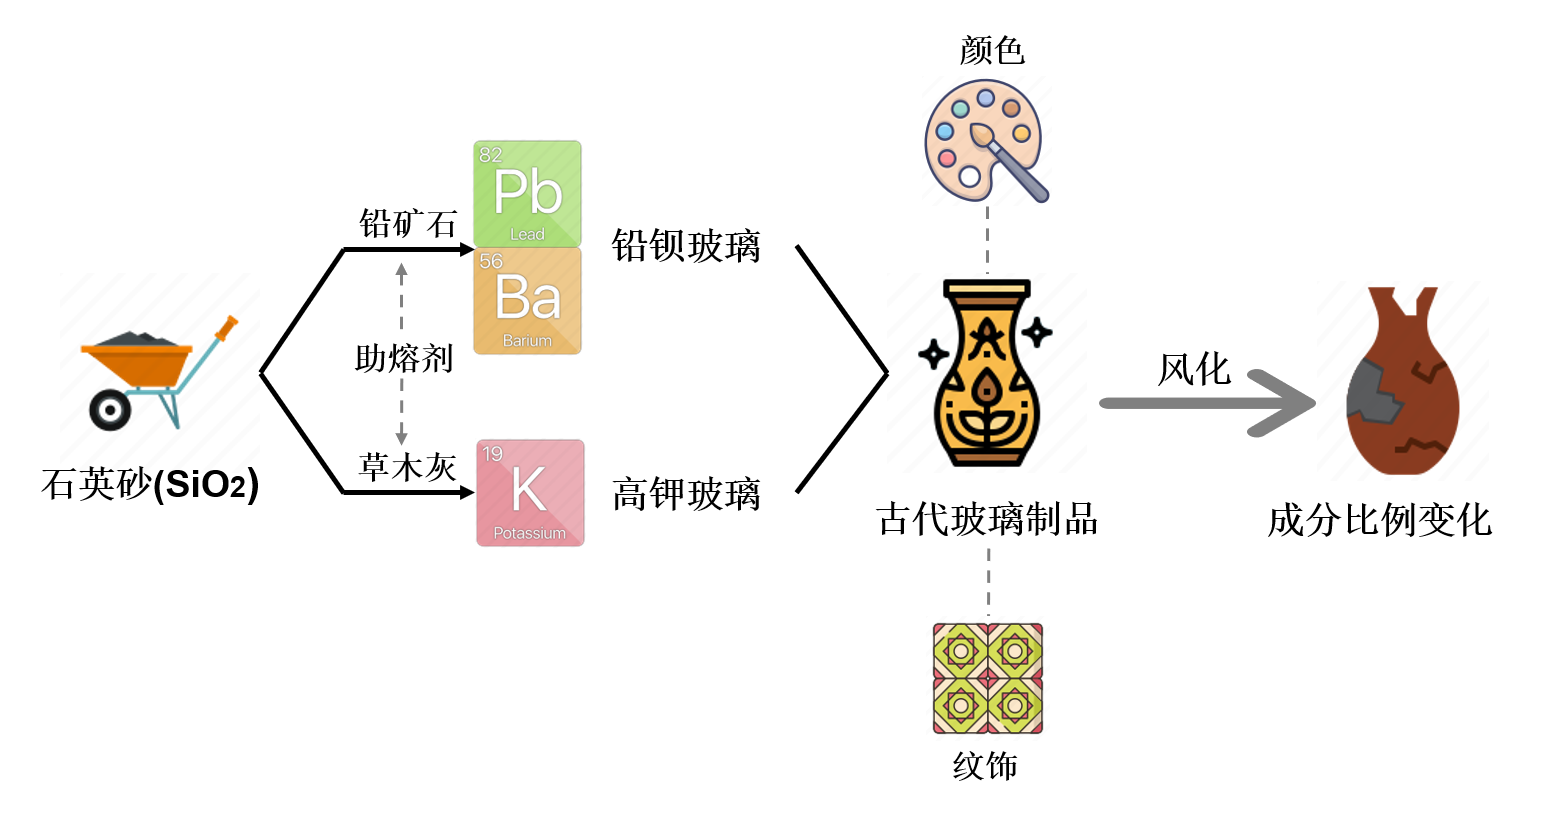
\includegraphics[width=0.9\textwidth]{figure/背景}
\caption{我国古代玻璃制品背景图}
\end{figure}

\subsection{问题提出}

现有一批我国古代玻璃制品的相关数据,将玻璃文物分为铅钡玻璃和高钾玻璃两种类型。针对我国古代玻璃制品化学成分与类别相关信息,我们对以下几个问题进行研究:

问题一:分析玻璃文物表面风化情况与其玻璃类型、纹饰以及颜色的关系,并依据玻璃类型对玻璃文物表面风化情况以及化学成分含量进行分析。之后结合风化点的数据对风化前该文物的成分含量进行预测。

问题二:结合数据探讨高钾玻璃、铅钡玻璃这两类玻璃制品的分类规律,并针对不同类别的玻璃制品进行基于化学成分的亚类划分。由此得到具体划分方式与结果,并进行合理性和敏感性分析。


问题三:分析附件表单 3 中文物的化学成分进行分析,判断各玻璃文物所属类别,并对分类结果进行敏感性分析。

问题四:分析不同类别玻璃文物化学成分间关联,并比较分析关联关系的差异性。



%----------- 二、模型假设 ----------
\section{模型假设}
(1)所有数据真实可靠;

(2)古代玻璃文物中同一文物各部位成分组成基本相同;

(3)所有玻璃制品的出土时间和地点对风化没有影响;

(4)未检测出的化学成分含量为0。



%----------- 三、符号说明 ----------
\section{符号说明}
\begin{table}[H]%htbp表示的意思是latex会尽量满足排在前面的浮动格式,就是h-t-b-p这个顺序,让排版的效果尽量好。
    \centering
    \begin{threeparttable}   
    \begin{tabular}{p{2.0cm}<{\centering}p{7.0cm}<{\centering}p{7.0cm}<{\centering}}
 %指定单元格宽度, 并且水平居中。
    \toprule[1.5pt]
    符号 & 含义 & 说明 \\ %换行 
    \hline
    $df$ & 自由度 & 卡方检验中两个变量对应的自由度 \\ %把你的符号写在这
    $e_{ij}$ & $i$风化情况和$j$类型玻璃对应理论频数 &  $i=1,2;j=1,2$ \\ %把你的符号写在这
    $X,Y$ & 回归自变量与因变量数据矩阵 &  $X=(x_{ij})_{n\times m}$,$Y=(y_{ij})_{n\times m}$  \\ %把你的符号写在这
   $p$ & Logistic回归玻璃类型为铅钡玻璃概率 &     \\ %把你的符号写在这
    $v_j$ & 第$j$项化学成分的信息熵 & $j=1,2,\cdots,14$  \\ %把你的符号写在这
    $\gamma_i$ & 灰色关联度 &  $i=1,2,\cdots,14$  \\ %把你的符号写在这
    \bottomrule[1.5pt]
    \end{tabular}
     \begin{tablenotes}
        \footnotesize
        \item 注:未列出以及重复的符号均以首次出现处为准
      \end{tablenotes}
  \end{threeparttable}
\end{table}

\section{问题一的模型建立与求解}

\subsection{问题一的描述与分析}

问题一要求分析玻璃文物表面风化情况与玻璃类型、纹饰及颜色的关系,并依据玻璃类型对表面风化情况及化学成分含量进行分析,结合风化点的数据对风化前该文物的成分含量进行预测。首先,基于题干条件进行\textbf{数据预处理},本文对于表单1与表单2中的缺失值与异常值分别进行处理。

针对表面风化与三项特征指标的关系分析,本文首先对不同玻璃类型、纹饰以及颜色下的表面风化数据分布情况进行初步分析。之后,利用\textbf{卡方独立性检验}对表面风化情况与三项特征变量的关联显著性进行分析。最终,本文结合数据特征以及卡方检验结果对数据进行\textbf{降维}处理,最终得到36种特征组合,结合不同组合下的表面风化情况对特征组合与表面风化的关系进行深入探讨。

针对表面有无风化化学成分含量统计规律的分析,本文从从描述性统计分析、化学成分含量数据分布分析、Mann-Whitney检验\textbf{三个维度}进行分析。基于Mann-Whitney检验结果以及\textbf{机理分析},得出不同类型玻璃的主要影响成分,并由此进行后续的预测。

针对风化前化学成分含量的预测,首先结合不同类型玻璃化学成分含量的统计规律确定\textbf{基准化匹配策略},从而对风化与未风化数据进行匹配。以筛选所得主要影响成分为重要指标进行回归分析,由于指标数量仍较大且样本数据量较小,本文以风化前的化学成分含量为因变量,风化后的相应化学成分为自变量,建立\textbf{偏最小二乘回归模型}预测。

\begin{figure}[H]
\centering
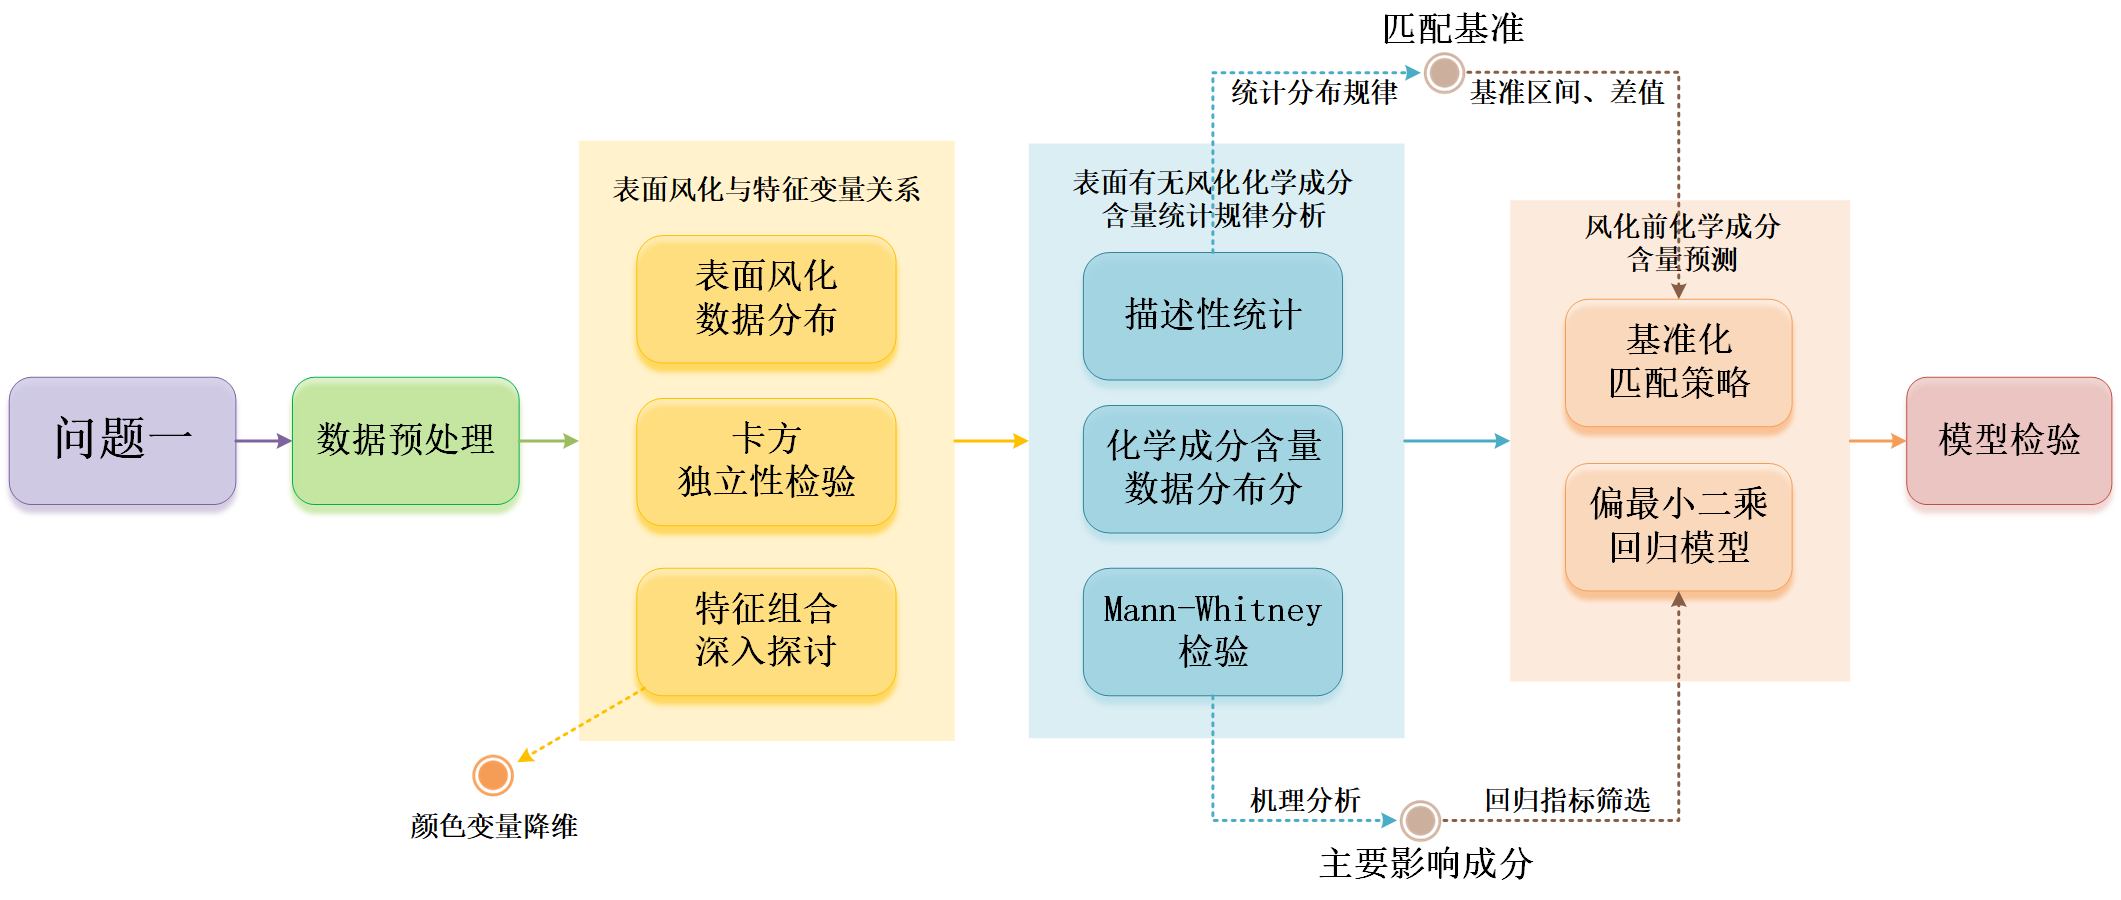
\includegraphics[width=1.05\textwidth]{figure/问题一}
\caption{问题一思路图}
\end{figure}

\subsection{数据预处理}

对于表单1中4项玻璃颜色为空白的数据,将其记为“未检测出颜色”,本文判断该情况的出现是由于风化程度较大从而导致文物颜色无法检测。对于表单2中的空白数据,本文将其认定为检测所得化学成分含量为0的情况。对于表单2中成分比例累加和不介于85$\% \sim 105\%$之间的数据,本文结合题干信息将其视为无效数据,予以删除。

\subsection{模型建立}

\subsubsection{基于卡方独立性检验的关系分析模型}

问题一要求分析表面风化情况与玻璃类型、纹饰和颜色三个玻璃特征变量的关系。由于玻璃纹饰与颜色的数据均为多类别变量,本文选择卡方独立性检验对表面风化情况与三项玻璃特征变量的关系进行分析。卡方独立性检验常用于研究两类变量间的关联性与依存性\textsuperscript{\cite{ref3}}。本文以表面风化情况与玻璃类型的卡方独立性检验为例,检验假设为:

$H_0$:表面风化情况与玻璃类型变量相互独立。表面风化情况与玻璃类型两个变量含有不同水平,表面风化情况有“风化”与“无风化”两个水平,玻璃类型变量有“铅钡”与“高钾”两个水平。自由度满足下式:
\begin{equation}
df = (R-1)(C-1).
\end{equation}
其中,$R$为行数,$C$为列数。对于分析表面风化情况与玻璃类型变量关系的情况,$R=2$,$C=2$。设$X_i$表示表面风化情况,$X_1$为风化,$X_2$为无风化。设$Y_j$表示两种不同类型的玻璃文物,$Y_1$、$Y_2$分别表示铅钡玻璃与高钾玻璃。结合$i$风化情况和$j$类型的玻璃文物对应的理论频数$e_{ij}$,由此计算统计量$\chi ^ { 2 }$,查表确定接受域。

分析表面风化情况与玻璃纹饰变量关系时,上述$R = 2$,$C = 3$;分析表面风化情况与玻璃纹饰变量关系时,上述$R = 2$,$C = 9$。其余检验步骤与上述分析类似。

\subsubsection{基于Mann-Whitney检验的统计规律分析模型}\label{mw}

由于不同化学成分含量数据不符合正态分布,本文选择独立样本Mann-Whitney检验对表面有无风化化学成分含量的统计规律分别进行分析\textsuperscript{\cite{ref2}}。以二氧化硅为例,检验假设为:$H_0$:表面风化与无风化二氧化硅含量的总体分布相同。

先将表面风化与无风化样本中二氧化硅含量的数值由小到大统一编秩,将两组秩分别相加得每组秩和。取任意一组样本(如表面风化)的秩和作为检验统计量$W$,在$H_0$假设成立情况下,则$W$的均值满足下式:
\begin{equation}
\mu_W = \frac{n_1(N+1)}{2}.
\end{equation}
其中,$n_1$表示表面风化样本数量,$N$表示样本总数。当$W$远离其均值时,则有理由拒绝$H_0$假设,认为两组有差异。由此得到$P$值并与显著性水平$\alpha$进行比较,对表面有无风化情况下二氧化硅含量的差异性进行分析。

对于其他化学成分含量,与上述检验步骤相同,最终得到表面有无风化情况下不同化学成分含量的差异性,并基于检验结果与机理分析筛选后续用于预测的指标。

\subsubsection{基于基准化匹配策略与偏最小二乘回归的成分含量预测模型}
\label{jizhun}

\begin{itemize}
  \item \textbf{表面有无风化数据的基准化匹配策略}
\end{itemize}

问题一要求根据风化点检测数据预测风化前的化学成分含量,而分析表单2中的数据发现,表面有无风化的数据不存在明显的对应关系。为了后续的预测工作,需要对同类型玻璃表面风化与无风化的数据进行匹配。本文将风化表面的无风化点视为无风化数据。首先,本文确定匹配策略的核心思想为匹配结果应遵循该类玻璃的统计与分布规律,即分析化学成分含量数据所得统计规律。

由于不同化学成分含量变化与表面风化的关联程度不一致,选择数据变化趋势作为基准显然是不合理的。因此,为保证基准选择的稳健性与有效性,本文利用估计总体中心的中位数统计量进行评估与匹配。确定基准化匹配的核心基准为:表面有无风化化学成分含量中位数之差。此外,结合铅钡玻璃与高钾玻璃不同的数据特征,本文对匹配基准进行适当的个性化处理,得到不同类型玻璃的基准化匹配策略如下:

$\circ$铅钡玻璃:分析表单2中铅钡玻璃对应数据发现,文物采样点49、50处存在两组理想匹配点,即同一采样点同时存在风化与未风化数据。设理想匹配点风化前后化学成分含量差值分别为$a_1$、$a_2$,铅钡玻璃该化学成分风化前后中位数之差为$a_0$。确定基准区间满足:
\begin{equation}
 [b_1,b_2] = [\min\{a_0,a_1,a_2\},\max\{a_0,a_1,a_2\}].
\end{equation}
基于该基准区间定义匹配距离$d_{ij}$,满足下式:
\begin{equation}
 d_{ij} = \begin{cases}
  0, & {\vartriangle m_{ij} \in [b_1,b_2],}\\
  {\vartriangle m_{ij} - b_2,} & {\vartriangle m_{ij} > b_2,}\\
  {b_1 - \vartriangle m_{ij},} & {\vartriangle m_{ij} < b_1.}
 \end{cases}
\end{equation}
其中,$m_{ij}$表示第$i$个风化前与第$j$个风化后化学成分含量数据之差。由于严重风化玻璃特征发生较大改变,本文不予匹配,则有$i = 1,2,\cdots,23$,$j = 1,2,\cdots,23$。比较$529$个匹配组合对应的匹配距离之和,所得最小值对应的匹配组合即为该化学成分匹配结果。对于铅钡玻璃对应的其他化学成分含量,同样进行上述匹配过程,最终得到匹配结果。

$\circ$高钾玻璃:分析表单2中高钾玻璃对应数据发现,并不存在与铅钡玻璃类似的理想匹配点。设化学成分含量中位数之差为$g_0$,即为基准中位数差值。定义匹配距离和$h_{ij}$,满足下式:
\begin{equation}
 h_{ij} = |\vartriangle r_{ij} - g_0|.
\end{equation}
其中,$r_{ij}$表示第$i$个风化前与第$j$个风化后化学成分含量数据之差。高钾玻璃具有12项未风化数据,6项风化数据,则有$i = 1,2,\cdots,12$,$j = 1,2,\cdots,6$。比较$72$个匹配组合对应的匹配距离之和,所得最小值对应的匹配组合即为该化学成分匹配结果。其余化学成分同样进行该过程。


\begin{itemize}
\item \textbf{偏最小二乘回归预测风化前化学成分含量}
\end{itemize}

由于筛选后指标数量仍较大且数据量较小,本文建立偏最小二乘法回归模型进行后续的预测分析以减弱指标间的多重共线性。本文以玻璃风化前的化学成分含量为因变量,以风化后的相应化学成分含量为自变量,建立偏最小二乘法回归模型\textsuperscript{\cite{ref4}}。设自变量观测数据矩阵为$X=(x_{ij})_{n\times m}$,因变量观测数据矩阵为$Y=(y_{ij})_{n\times m}$,$n$为样本总量,$m$为自变量个数,同样为因变量个数。

首先,将各指标$x_{ij}$转化为指标值$x_{ij}^*$,有:

\begin{equation}
  x_{ij}^*=\frac{x_{ij}-u_{j}^{(1)}}{s_{j}^{(1)}},\quad i = 1,2,\cdots,n;j = 1,2,\cdots,m.
\end{equation}
其中,$u_{j}^{(1)}$、$s_{j}^{(1)}$为第$j$个自变量$x_j$的样本均值和样本标准差。同理可得标准化指标$y_{ij}^*$。

计算标准化处理后的$m$个自变量与$m$个因变量之间的相关系数矩阵,由此将得到的$u_i$代入$y_j^*$的回归方程,得到标准化指标变量之间的回归方程。之后,将标准化变量$y_j^*$、$x_j^*$分别还原成原始变量$y_j$、$x_j$,得到回归方程。对于铅钡玻璃中的严重风化与风化数据,本文同样通过上述过程进行回归。

\subsection{模型求解与结果分析}

\subsubsection{表面风化与类型、纹饰和颜色的关系}

\begin{itemize}
	\item \textbf{表面风化数据分布分析}
\end{itemize}

首先,本文对不同玻璃类型、纹饰以及颜色下表面风化数据的分布情况进行初步分析。上述三项特征变量对应的数据分布如下图\ref{fenbu}:

\begin{figure}[H]
\centering
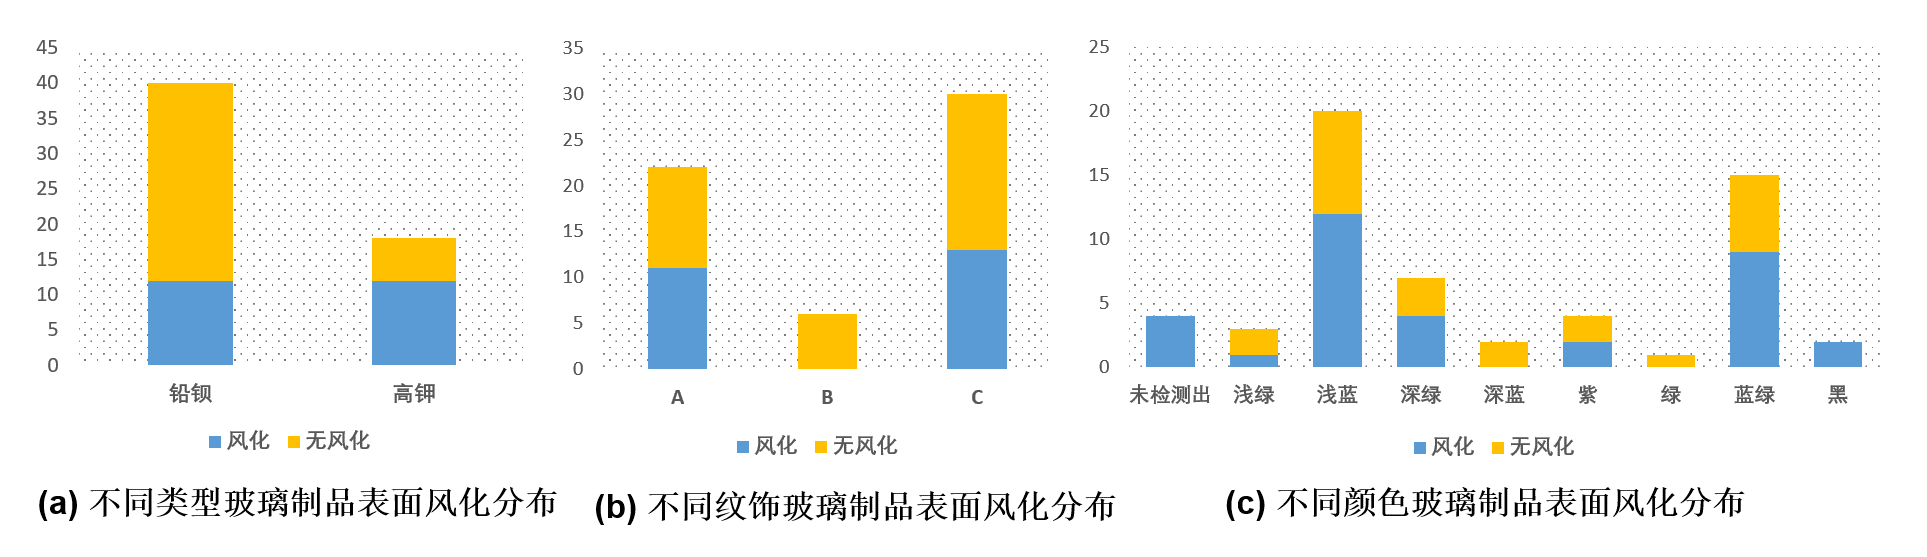
\includegraphics[width=1.05\textwidth]{figure/分布}
\caption{不同情况下表面风化数据分布图}
\label{fenbu}
\end{figure}

由上图(a)可知,高钾玻璃中发生表面风化的数据占比大于铅钡玻璃,该分布情况初步反映了玻璃制品的不同类型对表面风化情况存在影响。由图(b)可知,不同纹饰的玻璃制品对应的风化情况数据分布也存在差异,尤其体现在B纹饰中,该纹饰玻璃制品均无风化,说明B纹饰对可能对表面风化存在负向影响。而A纹饰风化与无风化玻璃比例趋近于1:1,说明该纹饰对表面风化的影响较小。由图(c)可知,不同颜色的玻璃制品对应的风化情况数据同样存在较大差异,其中未检测出颜色的玻璃制品均表现为风化,这是由于风化严重的玻璃制品外观与性状均发生较大变化,已无法检测出颜色。

综合分析,不同类型、纹饰以及颜色的玻璃制品对应的表面风化情况也存在不同,因此进一步分析表面风化情况与玻璃类型、纹饰与颜色的关系是有必要的。

\begin{itemize}
	\item \textbf{卡方独立性检验}
\end{itemize}

本文利用spss软件对表面风化情况与玻璃类型、纹饰、颜色三项特征变量分别进行卡方独立性检验,检验结果如下表:
\begin{table}[H]
\centering
\caption{表面风化与各特征变量卡方检验结果表}
\begin{threeparttable} 
\begin{tabular}{cccc}
\toprule[1.5pt]
指标 & $\chi^{2}$    & 校正$\chi^{2}$  & $P$        \\ \hline
颜色 & 9.432 & 9.432 & 0.307    \\
类型 & 6.88  & 5.452 & 0.009*** \\
纹饰 & 4.957 & 4.957 & 0.084*   \\ \bottomrule[1.5pt]
\end{tabular}
\begin{tablenotes}
        \footnotesize
        \item 注:***、*分别代表1$\%$、10$\%$的显著性水平
      \end{tablenotes}
  \end{threeparttable}
\end{table}
观察表中数据发现,在1$\%$的显著性水平下拒绝了表面风化与类型相互独立的原假设,在10$\%$的显著性水平下拒绝了表面风化与纹饰相互独立的原假设。由该结果可知,玻璃类型与表面风化的关联表现最显著,其次为玻璃纹饰与表面风化的关系,而颜色与表面风化的关联表现最不显著。

\begin{itemize}
	\item \textbf{特征组合关系的深入探讨}
\end{itemize}

最终,本文对不同玻璃类型、纹饰、颜色特征组合下的表面风化情况进行深入探讨。不同特征组合下表面风化变量均值以及该组合的样本数量(n)展示如下表(样本数量为0的特征组合不予展示):

\begin{table}[H]
\centering
\caption{不同特征组合下表面风化均值表}
\begin{tabular}{cccccc}
\toprule[1.5pt]
特征组合(类型,纹饰,颜色) & 均值   & n & 特征组合       & 均值                   & n                 \\ \hline
铅钡,A,未检测出颜色    & 1    & 2    & 铅钡,C,紫               & 0.5                  & 4                    \\
铅钡,A,蓝绿        & 1    & 1    & 铅钡,C,绿               & 0.5                  & 10                   \\
铅钡,A,黑         & 1    & 2    & 高钾,A,蓝               & 0                    & 1                    \\
高钾,B,蓝绿        & 1    & 6    & 高钾,A,蓝绿              & 0                    & 5                    \\
铅钡,C,未检测出颜色    & 1    & 2    & 高钾,C,绿               & 0                    & 1                    \\
铅钡,C,蓝         & 1    & 6    & 高钾,C,蓝               & 0                    & 4                    \\
铅钡,C,蓝绿        & 1    & 2    & 高钾,C,蓝绿              & 0                    & 1                    \\
铅钡,A,蓝         & 0.55 & 11   & \multicolumn{1}{l}{} & \multicolumn{1}{l}{} & \multicolumn{1}{l}{} \\ \bottomrule[1.5pt]
\end{tabular}
\end{table}

其中,对特征变量进行组合可得$2 \times 3 \times 9 = 54$种特征组合,而玻璃制品的样本总量为58,因此需对特征组合进行重新划分以达到更好的分析效果。由上述卡方检验结果可知玻璃颜色与表面风化的关联表现不显著,我们判断该结果是由于颜色变量的种类过多导致的。因此,本文结合古代玻璃的主要显色情况对颜色变量进行数据降维处理,将“深蓝”、“蓝”、“浅蓝”合并为“蓝”,将“深绿”、“浅绿”合并为“绿”,由此将9种颜色种类降至6种,最终得到$2 \times 3 \times 6 = 36$种特征组合。将表面风化变量记为“1”,无风化记为“0”,利用Excel软件计算不同特征组合下表面风化情况对应的均值,从而分析不同特征组合联合作用对表面风化情况的影响。

分析上表中表面风化均值为1的特征组合,即表现出风化的特征组合发现,特征组合在玻璃类型上表现出趋同性,大部分为铅钡玻璃,而在玻璃纹饰和颜色上并无明显规律。由此可知不同特征组合内部的复合作用较为复杂,各项因素交互影响从而导致风化的结果。分析上表中表面风化均值为0的特征组合发现,特征组合在玻璃类型上大多体现为高钾玻璃,而在玻璃纹饰和颜色上并无明显的趋同性。

\subsubsection{表面有无风化化学成分含量统计规律分析}

\begin{itemize}
	\item \textbf{描述性统计分析}
\end{itemize}

首先,本文利用Python软件对表面有无风化情况下各化学成分含量进行描述性统计分析,以高钾玻璃为例,表面有无风化化学成分含量的相关统计量如下表:
\begin{table}[H]
\centering
\caption{高钾玻璃表面有无风化化学成分含量描述性统计表}
\begin{tabular}{cccccccccc}
\toprule[1.5pt]
\multirow{2}{*}{统计量} &             & 无风化   & (n=12) &      &  &                  & 风化    & (n=6) &                  \\ \cline{2-5} \cline{7-10} 
                     & 样本区间        & 平均值   & 标准差    & 变异系数 &  & 样本区间             & 平均值   & 标准差   & 变异系数             \\ \hline
二氧化硅                 & 59.0-87.1 & 67.98 & 8.76   & 0.13 &  & 92.4-96.8      & 93.96 & 1.73  & 0.02             \\
氧化钠                  & 0-3.4      & 0.70  & 1.29   & 1.85 &  & \textbackslash{} & 0.00  & 0.00  & \textbackslash{} \\
氧化钾                  & 0-14.5     & 9.33  & 3.92   & 0.42 &  & 0-1.0           & 0.54  & 0.45  & 0.82             \\
氧化钙                  & 0-8.7       & 5.33  & 3.09   & 0.58 &  & 0.2-1.7        & 0.87  & 0.49  & 0.56             \\
氧化镁                  & 0-2.0      & 1.08  & 0.68   & 0.63 &  & 0-0.7           & 0.20  & 0.31  & 1.56             \\
氧化铝                  & 3.1-11.2  & 6.62  & 2.49   & 0.38 &  & 0.8-3.5         & 1.93  & 0.96  & 0.50             \\
氧化铁                  & 0-6.0      & 1.93  & 1.67   & 0.86 &  & 0.2-0.4        & 0.27  & 0.07  & 0.26             \\
氧化铜                  & 0-5.1      & 2.45  & 1.66   & 0.68 &  & 0.6-3.2        & 1.56  & 0.93  & 0.60             \\
氧化铅                  & 0-1.6      & 0.41  & 0.59   & 1.43 &  & \textbackslash{} & 0.00  & 0.00  & \textbackslash{} \\
氧化钡                  & 0-2.9      & 0.60  & 0.98   & 1.64 &  & \textbackslash{} & 0.00  & 0.00  & \textbackslash{} \\
五氧化二磷                & 0-4.5       & 1.40  & 1.43   & 1.02 &  & 0-0.6           & 0.28  & 0.21  & 0.75             \\
氧化锶                  & 0-0.1      & 0.04  & 0.05   & 1.16 &  & \textbackslash{} & 0.00  & 0.00  & \textbackslash{} \\
氧化锡                  & 0-2.4      & 0.20  & 0.68   & 3.46 &  & \textbackslash{} & 0.00  & 0.00  & \textbackslash{} \\
二氧化硫                 & 0-0.5      & 0.10  & 0.19   & 1.82 &  & \textbackslash{} & 0.00  & 0.00  & \textbackslash{} \\ \bottomrule[1.5pt]
\end{tabular}
\end{table}

由上表可知,表面有无风化高钾玻璃中二氧化硅的含量均占最大比重,而风化情况下的含量均值较无风化情况下增加了25.98,说明了风化对于二氧化硅含量的促进作用。此外,其他化学成分在表面有无风化情况下也存在较大差异,这是由于风化过程导致玻璃内部元素与环境元素交互作用,从而导致化学成分发生较大变化。以氧化钾为例,风化后该化学成分含量显著降低,而变异系数由0.42增大至0.82,即说明风化使该化学成分数据分布的离散程度增大。

\begin{itemize}
	\item \textbf{化学成分含量数据分布分析}
\end{itemize}

基于上述描述性统计分析,本文对各项描述性统计量数据区别较小的化学成分含量进行进一步分析,即对于含量较大的二氧化硅,以及含量极小氧化锶、氧化锡、二氧化硫,此处不予讨论。以高钾玻璃为例分析氧化纳、氧化钾、氧化钙、氧化镁等十项化学成分的含量分布。下图\ref{wufenghua}、图\ref{fenghua}分别展示表面无风化和有风化高钾玻璃化学成分分布情况:

\begin{figure}[H]
\centering
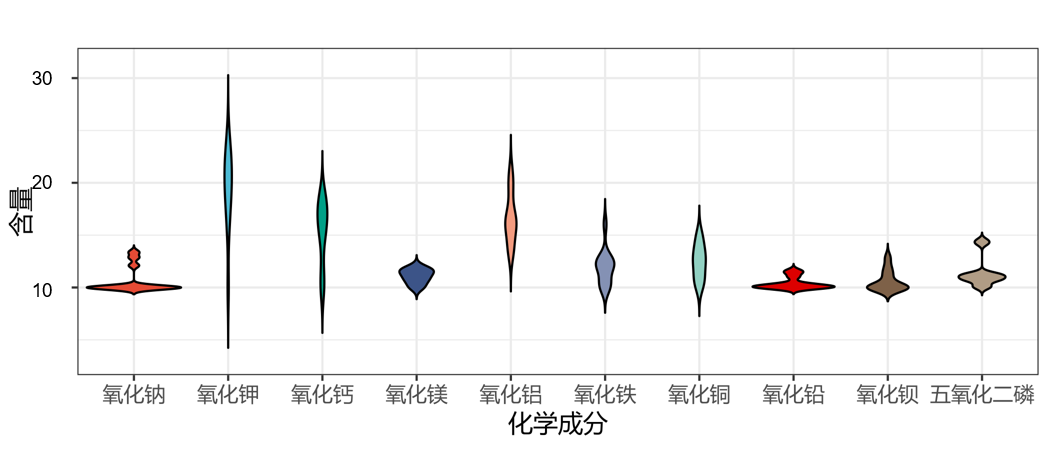
\includegraphics[width=0.9\textwidth]{figure/小提琴}
\caption{表面无风化高钾玻璃化学成分分布图}
\label{wufenghua}
\end{figure}

\begin{figure}[H]
\centering
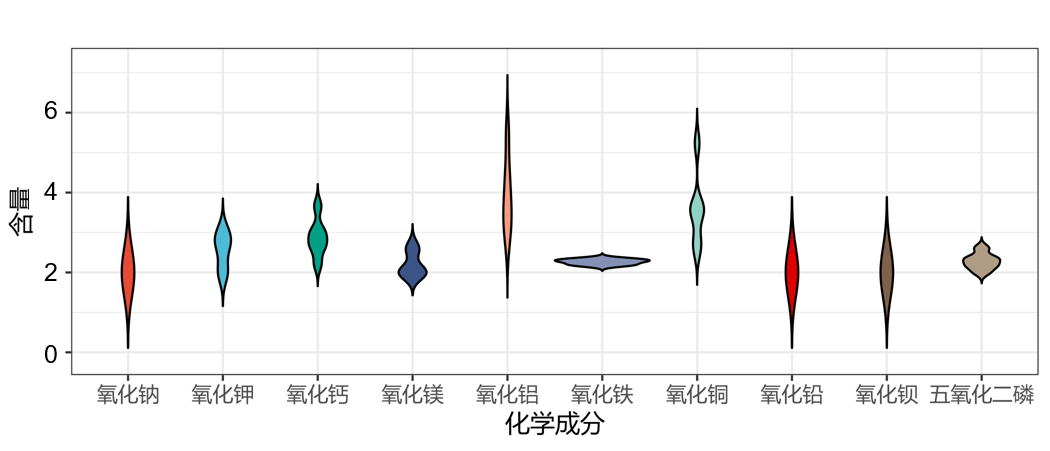
\includegraphics[width=0.9\textwidth]{figure/风化}
\caption{表面风化高钾玻璃化学成分分布图}
\label{fenghua}
\end{figure}

由图\ref{wufenghua}可知,表面无风化的高钾玻璃中,氧化钾、氧化钙、氧化铝、氧化铁、氧化铜在不同含量下的分布较为均匀。而对于氧化钠、氧化铅、氧化钡以及五氧化二磷,含量分布表现出集中于某一区域的现象。分析发现,分布较为均匀的化学成分均为玻璃制品的主要呈色元素,如使玻璃呈现绿色的铜离子、使玻璃呈现红色的铁离子等。该结果说明,对于无风化的玻璃来说,影响玻璃呈色的元素含量存在差异,即不同的个体具有一定的独特性。

由图\ref{fenghua}可知,表面风化的高钾玻璃中,上述玻璃制品的主要呈色元素数据分布较为集中,如氧化铁成分集中在0.2,不同个体的差异性表现不显著。该结果是由于风化促使玻璃制品的内部元素与环境元素进行大量交换,从而导致其成分比例发生变化,呈现出趋同性,而表现玻璃制品特异性的元素含量趋于相似。

\begin{itemize}
	\item \textbf{Mann-Whitney检验与机理分析}
\end{itemize}

本文对表面有无风化情况下不同种类化学成分含量的差异性进行Mann-Whitney检验,检验结果如下表:

\begin{table}[H]
  \centering
  \caption{Mann-Whitney检验结果表}
  \begin{threeparttable} 
  \begin{tabular}{ccccccc}
    \toprule[1.5pt]
    & 铅钡玻璃  &                   &           &       & 高钾玻璃          &                   \\ \cline{1-3} \cline{5-7} 
    变量名   & 统计量W  & p值                &           & 变量名   & 统计量W          & p值                \\ \hline
    二氧化硅  & 578   & \textbf{0.000***} & \textbf{} & 二氧化硅  & 0    & \textbf{0.000***} \\
    氧化钠   & 400   & \textbf{0.011**}  & \textbf{} & 氧化钠   & 45            & 0.194             \\
    氧化钾   & 367   & 0.143             &           & 氧化钾   & 67   & \textbf{0.004***} \\
    氧化钙   & 145   & \textbf{0.002***} & \textbf{} & 氧化钙   & 60   & \textbf{0.025**}  \\
    氧化镁   & 308   & 0.853             &           & 氧化镁   & 62   & \textbf{0.013**}  \\
    氧化铝   & 412   & \textbf{0.024**}  & \textbf{} & 氧化铝   & 71   & \textbf{0.000***} \\
    氧化铁   & 283.5 & 0.745             &           & 氧化铁   & 60   & \textbf{0.025**}  \\
    氧化铜   & 202   & 0.052*            &           & 氧化铜   & 48            & 0.261             \\
    氧化铅   & 47    & \textbf{0.000***} & \textbf{} & 氧化铅   & 57   & \textbf{0.035**}  \\
    氧化钡   & 267   & 0.521             &           & 氧化钡   & 48            & 0.123             \\
    五氧化二磷 & 107.5 & \textbf{0.000***} & \textbf{} & 五氧化二磷 & 62.5 & \textbf{0.013**}  \\
    氧化锶   & 191.5 & 0.031**           &           & 氧化锶   & 54            & 0.045**           \\
    氧化锡   & 312   & 0.62              &           & 氧化锡   & 39            & 0.48              \\
    二氧化硫  & 266   & 0.208             &           & 二氧化硫  & 45            & 0.194             \\ \bottomrule[1.5pt]
  \end{tabular}
\begin{tablenotes}
  \footnotesize
  \item 注:***、**、*分别代表1$\%$、5$\%$、10$\%$的显著性水平
\end{tablenotes}
\end{threeparttable}
\end{table}

由上表可知,对于铅钡玻璃,表面有无风化情况下二氧化硅、氧化钙、氧化铅、五氧化二磷的含量在1$\%$的显著性水平下表现出显著差异,氧化钠、氧化铝、氧化锶在5$\%$的显著性水平下表现出显著差异。对于高钾玻璃,二氧化硅、氧化钾、氧化铝的含量在1$\%$的显著性水平下表现出显著差异,氧化钙、氧化镁、氧化铁、氧化铅、五氧化二磷、氧化锶在5$\%$的显著性水平下表现出显著差异。

\textbf{机理分析:}基于上述Mann-Whitney检验结果,本文结合文献对铅钡玻璃与高钾玻璃分别进行机理分析,从而对上述检验结果进行佐证,并为后续预测过程筛选合适的自变量指标。结合参考文献\textsuperscript{\cite{ref1}},古代玻璃的化学成分被分为主要影响成分、非影响成分、微量元素以及着色剂元素四类。在古代玻璃的成分研究中,$Cu$是古代玻璃绿色、红色和蓝色的最主要显色元素之一。$Cu^{2+}$常被用作玻璃制备的着色剂,而$Sr^{2+}$常常为微量元素。由此,本文确定铅钡玻璃的主要影响成分为二氧化硅、氧化钙、氧化铅、五氧化二磷、氧化钠、氧化铝6项化学成分,高钾玻璃的主要影响成分为,二氧化硅、氧化钾、氧化铝、氧化钙、氧化镁、氧化铁、氧化铅、五氧化二磷8项化学成分。所得主要影响成分即为后续预测过程中针对不同类型玻璃筛选所得指标。

\subsubsection{风化前的化学成分含量预测}

\begin{itemize}
  \item \textbf{基准化匹配策略}
\end{itemize}

基于上述分析所得铅钡玻璃与高钾玻璃的主要影响成分,结合\ref{jizhun}中不同类型玻璃的基准化匹配策略,得到两种玻璃基准展示如下表:
\begin{table}[H]
  \centering
  \caption{铅钡玻璃与高钾玻璃匹配基准表}
  \begin{tabular}{ccccc}
    \toprule[1.5pt]
    \multicolumn{2}{c}{铅钡玻璃}     &  & \multicolumn{2}{c}{高钾玻璃} \\ \cline{1-2} \cline{4-5} 
    主要影响因素 & 基准区间                &  & 主要影响因素     & 基准中位数差值     \\ \hline
    二氧化硅   & {[}-29.60,-25.82{]} &  & 二氧化硅       & 27.975      \\
    氧化钠    & {[}-1.47,0{]}       &  & 氧化钾        & -9.165      \\
    氧化钙    & {[}0.07,2.50{]}     &  & 氧化钙        & -5.265      \\
    氧化铝    & {[}-2.29,-1.12{]}   &  & 氧化镁        & -1.165      \\
    氧化铅    & {[}11.16,23.94{]}   &  & 氧化铝        & -4.465      \\
    五氧化二磷  & {[}0,6.78{]}        &  & 氧化铁        & -1.835      \\
    &                     &  & 氧化铅        & -0.155      \\
    &                     &  & 五氧化二磷      & -0.74       \\ \bottomrule[1.5pt]
  \end{tabular}
\end{table}

基于上述基准,利用Matlab软件分别对表单2中铅钡玻璃与高钾玻璃表面有无风化数据进行匹配。匹配流程如下图\ref{pipei}:
\begin{figure}[H]
  \centering
  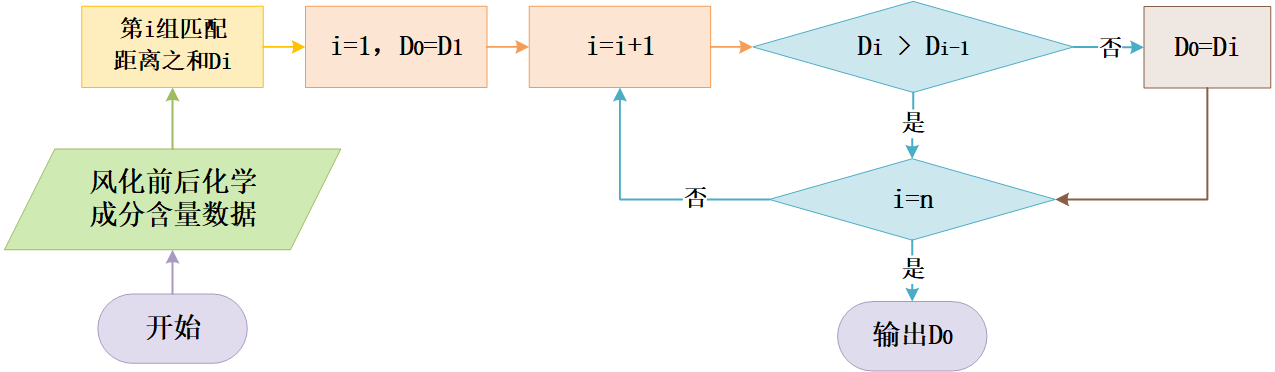
\includegraphics[width=0.8\textwidth]{figure/匹配}
  \caption{基准化匹配流程图}
  \label{pipei}
\end{figure}
图中$n$表示该类型玻璃匹配组合数量,对于铅钡玻璃$n=529$,对于高钾玻璃$n=72$。由此得到两种类型玻璃对应风化前后化学成分含量数据匹配结果见附录。

\begin{itemize}
  \item \textbf{偏最小二乘回归模型}
\end{itemize}

利用筛选所得的铅钡玻璃与高钾玻璃的主要影响成分,以及基准化匹配所得风化与未风化数据,进行偏最小二乘回归,得到不同类型玻璃风化前化学成分的回归方程。此外,本文利用08、26、54文物采样点处铅钡玻璃严重风化与风化的数据进行回归。完整的各化学成分含量回归系数见附录,此处以二氧化硅为例进行分析。

对于铅钡玻璃,求解得到回归方程为:
\begin{equation}
  \begin{aligned}
 y_{SiO_2} = 47.668 & +  0.531 \cdot x_{SiO_2} + 1.613 \cdot x_{Na_2O} - 0.474\cdot x_{CaO} \\ & -0.363\cdot x_{Al_2O_3}  -0.245\cdot x_{PbO} +0.318\cdot x_{P_2O_5} .
\end{aligned}
\end{equation}
其中,$y_{SiO_2}$为风化前二氧化硅含量,$x_{SiO_2},x_{Na_2O},x_{CaO},x_{Al_2O_3},x_{PbO}, x_{P_2O_5}$分别为风化后二氧化硅、氧化钠、氧化钙、氧化铝、氧化铅、五氧化二磷含量。

对于高钾玻璃,求解得到回归方程为:
\begin{equation}
  \begin{aligned}
    y_{SiO_2} = -92.082 & +  1.709 \cdot x_{SiO_2} - 3.519 \cdot x_{K_2O} +2.869 \cdot x_{CaO}  +2.06 \cdot x_{Al_2O_3} \\ & -5.17\cdot x_{MgO} -11.385 x_{Fe_2O_3} + 0.018 \cdot x_{PbO} -9.043 \cdot x_{P_2O_5} .
  \end{aligned}
\end{equation}
其中,$y_{SiO_2}$为风化前二氧化硅含量,$x_{SiO_2},x_{K_2O},x_{CaO},x_{Al_2O_3},x_{MgO},x_{Fe_2O_3},x_{PbO}, x_{P_2O_5}$分别为风化后二氧化硅、氧化钾、氧化钙、氧化铝、氧化镁、氧化铁、氧化铅、五氧化二磷含量。

分析上述回归方程发现,对于铅钡玻璃,风化后二氧化硅、氧化钠和五氧化二磷含量对风化前二氧化硅含量具有正向影响,而风化后氧化钙、氧化铝和氧化铅含量对其具有负向影响。对比回归系数发现,各指标对因变量的影响程度差距较小,进一步印证了本文指标筛选的合理性以及回归结果的可靠性。对于高钾玻璃,风化后二氧化硅、氧化钙、氧化铝、氧化铅对风化前二氧化硅含量具有正向影响,而风化后氧化钾、氧化镁、氧化铁、五氧化二磷对其具有负向影响。其中,氧化铁对二氧化硅的影响程度最大,本文判断该结果是由于$Fe^{3+}$元素具有显色作用,风化过程会造成玻璃制品颜色发生较大改变,因此该元素的含量会对玻璃制品最主要的元素二氧化硅含量造成较大影响。

对比铅钡玻璃与高钾玻璃的二氧化硅含量回归方程发现,对于相同自变量指标,相应的回归系数存在较大的差异性。如氧化铅含量对铅钡玻璃二氧化硅含量具有负向效应,而对于高钾玻璃则具有正向效应,该结果与玻璃类型的差异性相印证。

基于回归方程预测得到高钾玻璃和部分铅钡玻璃风化前二氧化硅含量如下表,完整预测结果以及其他化学成分预测结果见附录。

\begin{table}[H]
  \centering
  \caption{风化前二氧化硅含量表}
  \begin{tabular}{ccccc}
    \toprule[1.5pt]
    \multicolumn{2}{c}{高钾玻璃} &  & \multicolumn{2}{c}{铅钡玻璃} \\ \cline{1-2} \cline{4-5} 
    文物采样点     & 风化前二氧化硅      &  & 文物采样点     & 风化前二氧化硅      \\ \hline
    07        & 65.91963     &  & 02        & 53.25844     \\
    09        & 65.9207      &  & 08        & 51.28942     \\
    10        & 69.37144     &  & 11        & 59.62637     \\
    12        & 65.9206      &  & 19        & 53.03915     \\
    22        & 65.92005     &  & 26        & 51.00032     \\
    27        & 65.91966     &  & 34        & 54.41277     \\ \bottomrule[1.5pt]
  \end{tabular}
\end{table}

由上表可知,不同类型玻璃对应的预测结果较为接近,分别集中在65、55附近,体现了预测结果的稳健性与可靠性。此外,高钾玻璃各项化学成分预测对应的$R^2$均大于0.9,预测效果较好。铅钡玻璃中氧化钠对应$R^2$较低,这是由于氧化钠含量数据中存在较多0值,预测难度较大,而其余化学成分预测对应$R^2$均大于0.6,预测效果良好。

\subsection{模型检验}

题干中将化学成分比例累加和介于 $85\% \sim 105\%$之间的数据视为有效数据,由此本文对预测结果进行检验,对预测所得各化学成分含量进行累加如下图:
\begin{figure}[H]
  \centering
  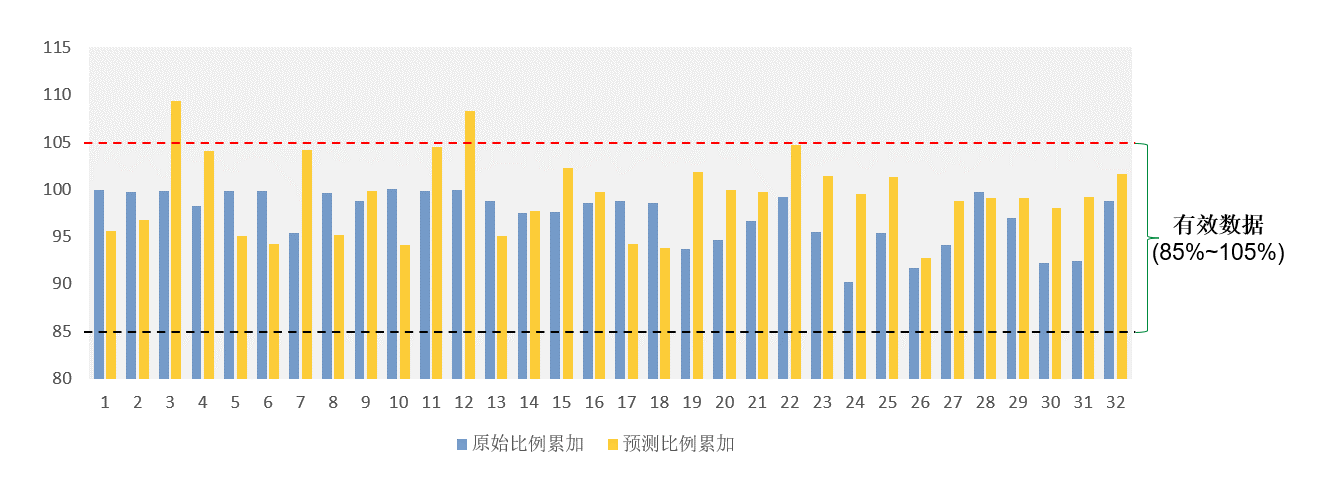
\includegraphics[width=1.1\textwidth]{figure/有效}
  \caption{表面风化高钾玻璃化学成分分布图}
  \label{youxiao}
\end{figure}

由上图可知,预测所得各化学成分累加结果中仅有两项数据超出有效数据范围,印证了本文确定的基准化匹配策略以及建立的预测模型的合理性,验证了预测结果的可靠性。

\section{问题二的模型建立与求解}

\subsection{问题二的描述与分析}

问题二要求结合数据探讨高钾玻璃、铅钡玻璃的分类规律。并基于化学成分针对不同类别的玻璃制品进行亚类划分,并对划分结果进行合理性与敏感性分析。本文首先对不同类型玻璃对应的化学成分含量差异进行Mann-Whitney检验,得到具有显著差异性的指标并进行\textbf{Logistic回归},进一步分析玻璃的分类规律。

在进行亚类划分前,本文首先对数据进行预处理,再基于\textbf{熵值法}与\textbf{均值乘数}得到量化权重从而选取划分指标。由此通过主成分分析法对所选指标进行\textbf{降维},并利用\textbf{K-Means++算法}对数据进行聚类从而确定亚类划分。其中,本文结合量化权重对聚类中的距离计算方法进行了改进。

最终,本文基于\textbf{Kruskal-Wallis检验}以及表面有无风化的亚类数据分布,对亚类划分结果的合理性进行分析,并基于量化权重调节进行敏感性分析。


\begin{figure}[H]
\centering
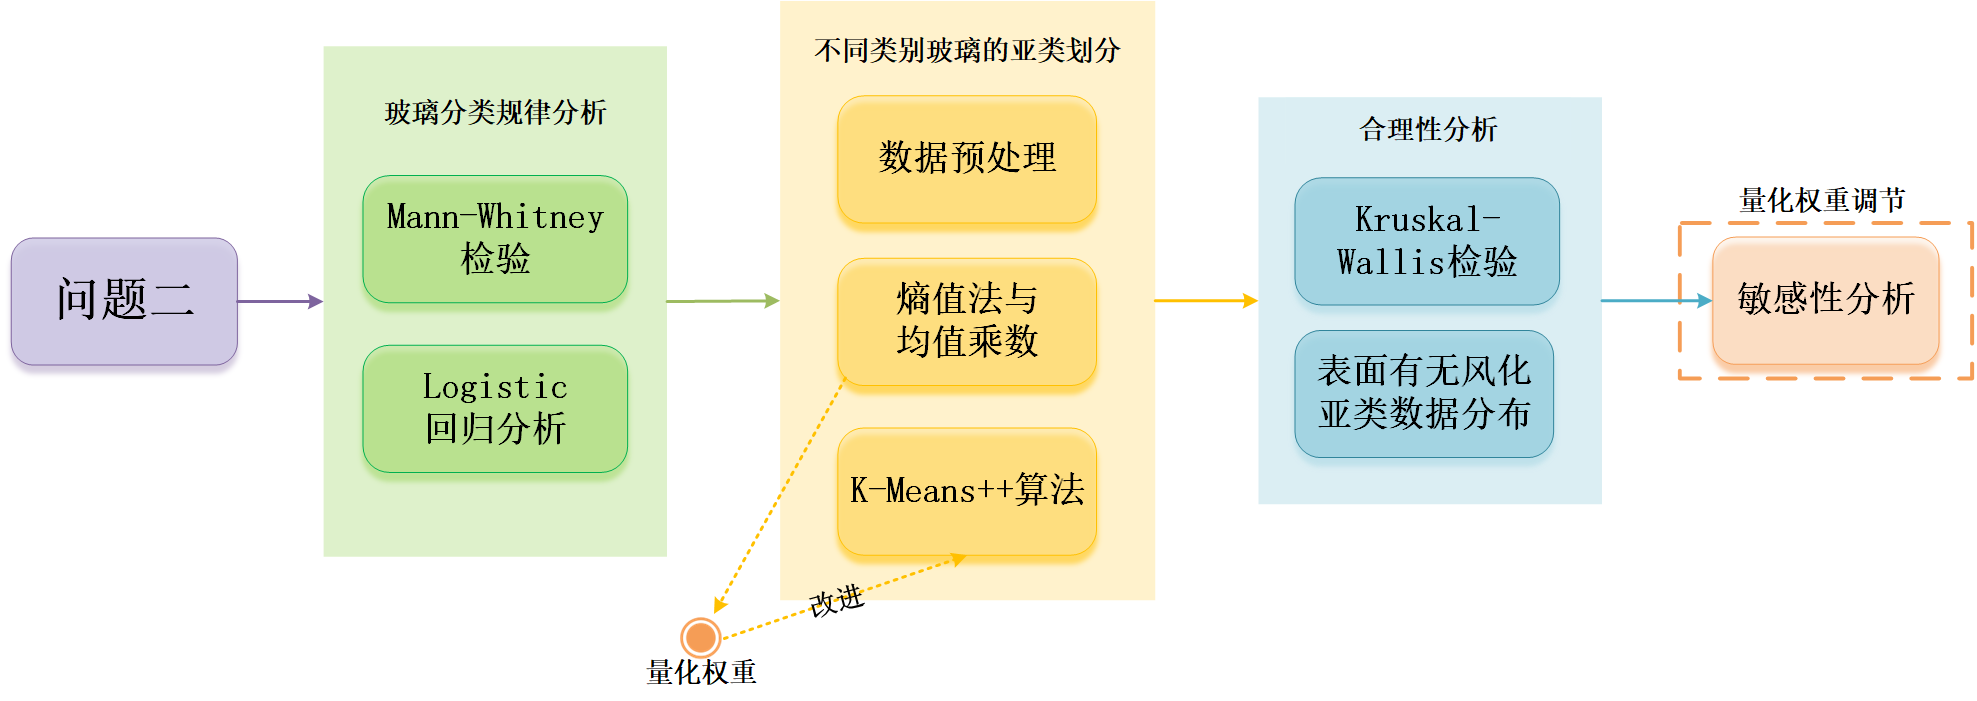
\includegraphics[width=1\textwidth]{figure/问题二}
\caption{问题二思路图}
\end{figure}


\subsection{模型建立}
\subsubsection{基于M-W检验与Logistic回归的分类规律分析模型}
问题二要求分析铅钡和高钾玻璃的分类规律,本文首先对不同类型玻璃对应的化学成分含量差异进行Mann-Whitney检验,具体检验步骤与\ref{mw}相同。基于Mann-Whitney检验结果对表现出显著差异的$n_0$个化学成分指标进行进一步分析。若将所有化学成分数据一起进行回归分析,会产生严重的多重共线性,从而导致变量均表现不显著的情况。因此,本文采用对各个变量依次回归的方式研究变量的分布对玻璃类型的影响。本文建立Logistic回归模型对化学成分数据进行回归分析,回归方程为\textsuperscript{\cite{ref6}}:
\begin{equation}
 ln \frac{p}{1-p} = \beta_{0i} + \beta_{1i} x_i,\quad (i = 1,2,\cdots,n_0).
\end{equation}
其中,$p$为玻璃类型为铅钡玻璃的概率,$x_i$为第$i$个显著化学成分指标,$\beta_{0i} , \beta_{1i}$为回归系数。基于回归结果分析玻璃的分类规律,即不同化学成分对玻璃类型的影响情况及影响程度。

\subsubsection{基于熵值法与K-Means++聚类的亚类划分模型}

\begin{itemize}
  \item \textbf{数据预处理}
\end{itemize}


在对玻璃制品进行亚类划分前,本文对表单2中数据进行以下预处理:

1. 由于需要分类的对象为古代玻璃制品,为了更好地利用亚类划分结果对玻璃制品所属朝代以及历史价值进行分析,应对表面风化前的化学成分含量进行分类与分析。因此,本文利用问题一中求解所得回归方程,将表单2中表面风化部位对应的化学成分含量转化为风化前数据。

2. 对所得风化前数据进行有效数据检验,即各化学成分比例累加和应介于  $85\% \sim 105\%$之间。对于不满足条件的数据,予以删除。

3. 为避免相似数据过多对后续聚类造成较大影响,本文对于表单2中同一文物上对应的数据取均值处理,以达到更好的分类效果。

\begin{itemize}
  \item \textbf{基于熵值法与均值乘数的划分指标选取}
\end{itemize}

首先对各项化学成分含量数据进行标准化处理,计算第$j$项化学成分的熵值$e _ { j }$为:
\begin{equation}
  e _ { j } = - \frac { 1 } { \ln n_w } \sum _ { i = 1 } ^ { n_w } p _ { i,j } \ln p _ { i,j },\quad (i=1,2,\cdots,n_w;j=1,2,\cdots,14).
\end{equation}
其中,$p_{i,j}$为第$j$项化学成分下第$i$个文物采样点占该指标的比重。

第$j$项化学成分的信息熵$v _ { j }$为:
\begin{equation}
  v _ { j } = \left\{ \begin{array} { l r } { ( 1 - \overline { e_j } ^ { \alpha } ) v _ {  j } + \overline { e_j } ^ { \alpha }\overline{ v _ {  j } },}&{ e _ { j } < 1 } \\ { 0 , } & { e _ { j } = 1 } \end{array} \right. .
\end{equation}
其中,$\overline{v_{j}}$为指标$m_j$的平均信息熵,$e_j$为对应的熵值,$\overline { e_j}$为全部不为1的熵值的平均值,$\alpha$为熵值指数,此处取文物采样点个数,对于铅钡玻璃取40,高钾玻璃取16。

由于含量极小的微量元素如氧化锶会对应的较大信息熵,为了避免该情况对划分指标的选取造成影响,本文引入均值乘数结合各指标信息熵最终得到不同化学成分的量化权重\textsuperscript{\cite{ref8}}。量化权重$u_j$的计算方法为:
\begin{equation}
 u_j = \sqrt{v_j \times \lambda_j}.
\end{equation}
其中,$\lambda_j$为第$j$项化学成分的均值乘数,即该化学成分在所有文物采样点的含量均值。

\begin{itemize}
  \item \textbf{基于K-Means++聚类的亚类划分}
\end{itemize}

K-means++算法在选择聚类中心时采用原则是保证初始聚类中心之间距离尽可能远,从而可以对K-means算法进行改进。本文首先利用主成分分析法对所选化学成分指标进行降维,接着选择K-means++算法对数据进行聚类,从而确定亚类划分\textsuperscript{\cite{ref7}}。其中,由于量化权重越高化学成分数据的离散程度越大,更易于亚类的划分,因此本文利用降维所得主成分的量化权重对与聚类中心的距离进行改进,将第$i$和第$j$个样本点间的距离表达式修改为加权距离:
\begin{equation}
 d^{\prime}(X_i,X_j) = \sqrt{{\sum_{t=1}^2} w_t {(F_{it}-F_{jt})}^2}.
\end{equation}
其中,$F_{it}$和$F_{jt}$分别表示样本点$i$和$j$在第$t$个主成分中的占比,$w_t$表示基于量化权重得到的第$t$个主成分的权重,满足下式:
\begin{equation}
 w_t = \sum_{j=1}^{5} F_t \cdot u_j,\quad t=1,2.
\end{equation}


基于加权距离的K-means++算法流程如下图\ref{julei}:
\begin{figure}[H]
  \centering
  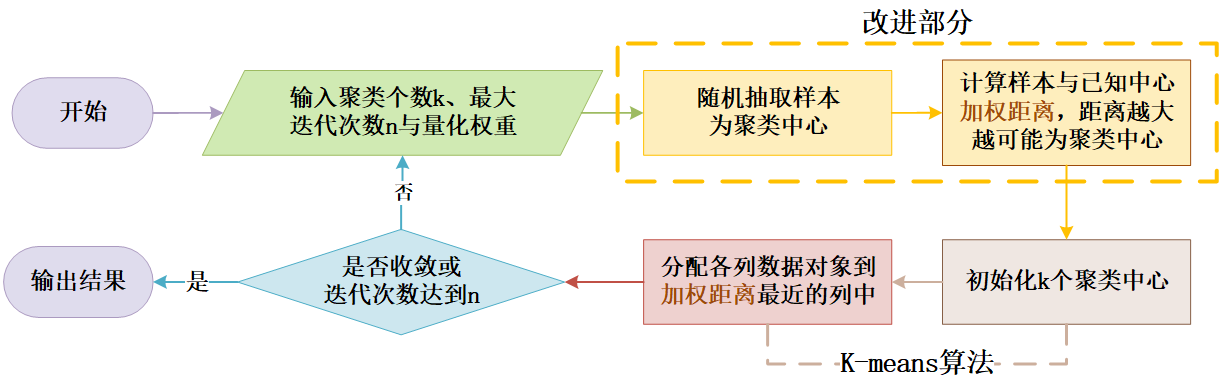
\includegraphics[width=1\textwidth]{figure/聚类}
  \caption{基于加权距离的K-Means++算法流程图}
  \label{julei}
\end{figure}


\subsection{模型求解与结果分析}

\subsubsection{玻璃分类规律分析}

不同玻璃类型对应化学成分含量差异的Mann-Whitney检验结果如下表:

\begin{table}[H]
  \centering
  \caption{不同玻璃类型Mann-Whitney检验结果表}
  \begin{threeparttable}
  \begin{tabular}{cccccc}
    \toprule[1.5pt]
    变量名  & p值       & Cohen's d值 & 变量名   & p值       & Cohen's d值 \\ \hline
    二氧化硅 & 0.000*** & 2.14       & 氧化铜   & 0.065*   & 0.122      \\
    氧化钠  & 0.341    & 0.267      & 氧化铅   & 0.000*** & 2.574      \\
    氧化钾  & 0.000*** & 2.286      & 氧化钡   & 0.000*** & 1.407      \\
    氧化钙  & 0.116    & 0.816      & 五氧化二磷 & 0.202    & 0.662      \\
    氧化镁  & 0.441    & 0.214      & 氧化锶   & 0.000*** & 1.407      \\
    氧化铝  & 0.050*   & 0.459      & 氧化锡   & 0.607    & 0.216      \\
    氧化铁  & 0.019**  & 0.63       & 二氧化硫  & 0.598    & 0.271      \\ \bottomrule[1.5pt]
  \end{tabular}
\begin{tablenotes}
  \footnotesize
  \item 注:***、**、*分别代表1$\%$、5$\%$、10$\%$的显著性水平
\end{tablenotes}
\end{threeparttable}
\end{table}

由上表可知,在1$\%$显著性水平下表现出显著差异的指标为二氧化硅、氧化钾、氧化铅、氧化钡、氧化锶。此外,Cohen's d值越大则该化学成分在不同类型玻璃下差异越显著。按照Cohen's d值从大到小进行排序如下图\ref{xianzhu}:

\begin{figure}[H]
  \centering
  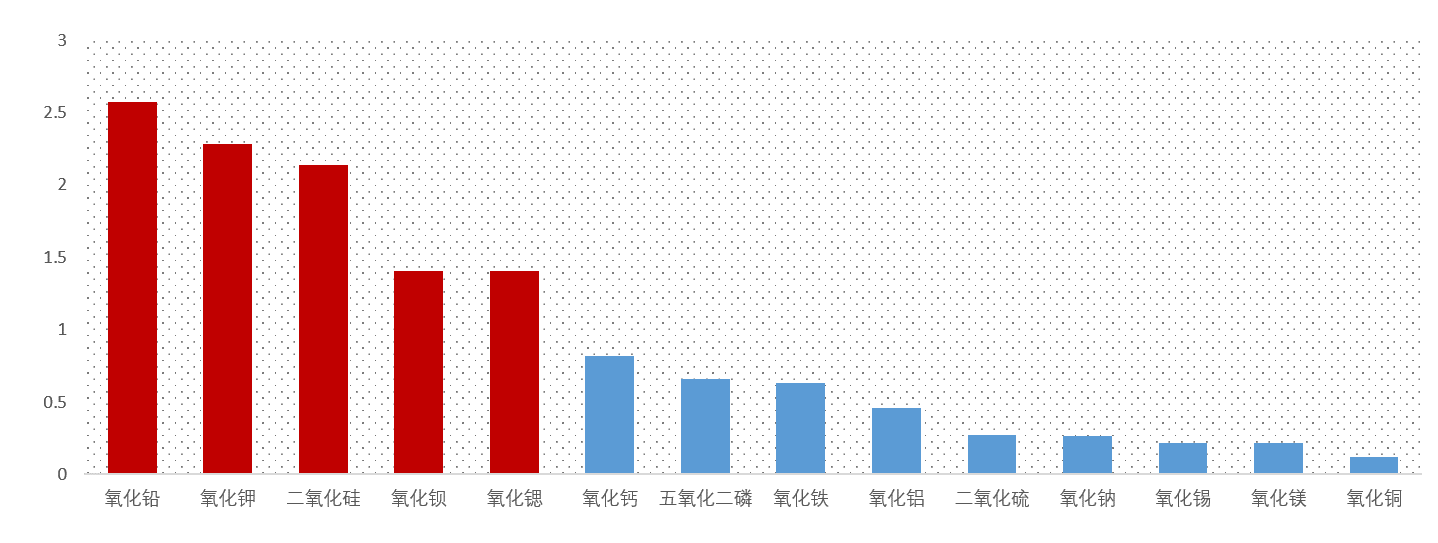
\includegraphics[width=1\textwidth]{figure/显著}
  \caption{化学成分指标Cohen's d值示意图}
  \label{xianzhu}
\end{figure}
上图中红色指标即为具有显著差异的化学成分指标,本文针对5项显著指标进行Logistic回归,进一步分析玻璃的分类规律。回归效果如下表:

\begin{table}[H]
  \centering
  \caption{Logistic回归效果表}
  \begin{tabular}{cccccc}
    \toprule[1.5pt]
    & 氧化铅   & 氧化钾   & 二氧化硅   & 氧化钡  & 氧化锶\\ \hline
    准确率 & 1 & 0.881 & 0.851 & 0.925 & 0.791   \\
    召回率 & 1 & 0.881 & 0.851 & 0.925 & 0.791   \\
    精确率 & 1 & 0.885 & 0.846 & 0.927  & 0.809   \\
    F1  & 1 & 0.872 & 0.844 & 0.926 & 0.797   \\
    影响  & 正向    & 负向    & 负向    & 正向    & 正向  \\ \bottomrule[1.5pt]
  \end{tabular}
\end{table}


比较表中准确率、召回率、精确率以及F1分数可知,氧化铅数据对玻璃类型的影响最大,即依据氧化铅含量进行玻璃类型划分是准确分类。基于回归方程可知,化学成分含量越大则铅钡玻璃概率越大,因此正向影响指的是该化学成分含量越大,玻璃类型越倾向于被划分为铅钡玻璃。如氧化铅含量越大,玻璃类型越可能为铅钡玻璃。结合数据可知,氧化铅含量大于9.3时,玻璃类型均为铅钡玻璃,因此可将氧化铅含量作为基类的判断标准,即由此对铅钡玻璃与高钾玻璃进行划分。

综合分析,玻璃的分类规律体现于氧化铅、氧化钾、二氧化硅、氧化钡以及氧化锶这5个化学成分的含量。氧化铅、氧化钡与氧化锶含量较高时,玻璃类型倾向于铅钡玻璃,含量较低时倾向于高钾玻璃。氧化钾和二氧化硅含量较高时,玻璃类型倾向于高钾玻璃,含量较低时倾向于铅钡玻璃。

\subsubsection{玻璃的亚类划分}

首先,对于铅钡玻璃与高钾玻璃分别进行基于熵值法与均值乘数的量化权重计算,得到两种玻璃各化学成分含量量化权重展示如下图\ref{qianbei}、图\ref{gaojia}:

\begin{figure}[H]
  \centering
  \begin{minipage}[t]{0.48\textwidth}
    \centering
    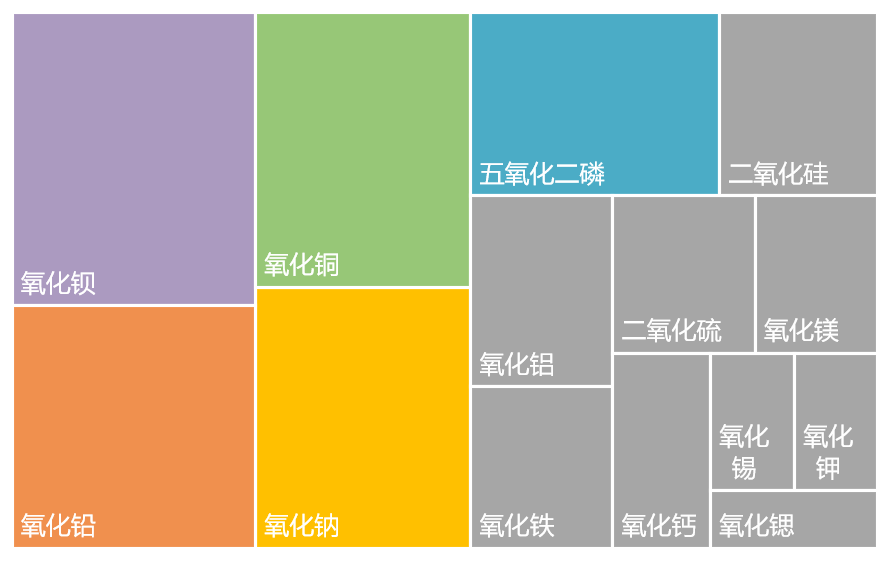
\includegraphics[width=7.5cm]{figure/铅钡}
    \caption{铅钡玻璃化学成分量化权重图}
    \label{qianbei}
  \end{minipage}
  \begin{minipage}[t]{0.48\textwidth}
    \centering
    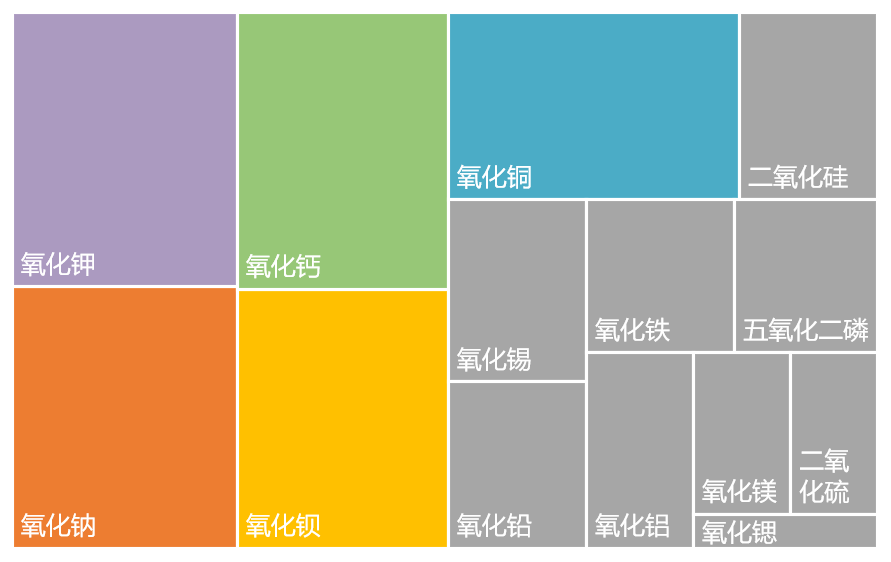
\includegraphics[width=7.5cm]{figure/高钾}
    \caption{高钾玻璃化学成分量化权重图}
    \label{gaojia}
  \end{minipage}
\end{figure}

为了选出能较全面反映该类玻璃特征的化学成分指标,本文选择量化权重之和大于60$\%$的化学成分指标作为该类玻璃的划分标准指标。对于铅钡玻璃,本文选择氧化钡、氧化铅、氧化铜、氧化钠、五氧化二磷五项化学成分指标为标准进行后续亚类划分,这五项指标对应量化权重之和为61.77$\%$。对于高钾玻璃,本文选择氧化钾、氧化钠、氧化钙、氧化钡、氧化铜五项化学成分指标为标准进行后续亚类划分,这五项指标对应量化权重之和为62.13$\%$。

由于选择的划分指标较多,为了避免K-Means++在高维空间上数据点之间距离关系弱化的问题,本文利用主成分分析法分别对两种类型玻璃对应的划分指标进行降维处理。


\begin{table}[H]
  \caption{主成分分析结果表}
  \centering
  \begin{tabular}{cccccccc}
    \toprule[1.5pt]
           & 特征向量 & 氧化钠    & 氧化铜    & 氧化铅    & 氧化钡    & 五氧化二磷  & 累积贡献率   \\ \hline
           & $r_1$   & -0.213 & \textbf{0.635}  & -0.208 & 0.607  & 0.374  & 60.19\% \\
           铅钡玻璃 & $r_2$   & \textbf{0.651}  & 0.158  & -0.496 & 0.209  & -0.511 & 84.91\% \\
           & $r_3$   & ...    & ...    & ...    & ...    & ...    & ...     \\
           & 特征向量 & 氧化钠    & 氧化钾    & 氧化钙    & 氧化铜    & 氧化钡    & 累积贡献率   \\
           & $r_1$   & -0.418 & \textbf{-0.574} & -0.455 & 0.118  & 0.524  & 52.14\% \\
           高钾玻璃 & $r_2$   & -0.285 & 0.118  & -0.424 & \textbf{-0.803} & -0.284 & 80.33\% \\
           & $r_3$   & ...    & ...    & ...    & ...    & ...    & ...     \\ \bottomrule[1.5pt]
  \end{tabular}
\end{table}

从上表中铅钡玻璃对应结果可以看出,前一个和前两个主成分的累计贡献率分别达到60.19$\%$和84.91$\%$,第一主成分$r_1$在氧化铜上都较大的负载荷,反映了玻璃的着色元素,因此第一主成分可称为着色成分。第二主成分$r_2$在变量氧化钠上有很高的正载荷,在氧化铅上有很大的负载荷。可以认为这个主成分度量了该类玻璃的主要元素,第二主成分可称为主要成分。而第三主成分很难给出明显的解释,因此我们只取前面两个主成分。对于高钾玻璃,同理将第一主成分称为主要成分,第二主成分称为着色成分。

数据降维后,对铅钡玻璃与高钾玻璃分别进行K-Means++算法聚类,针对本文K-means++聚类的$k$值确定,本文采用肘部法进行确定。肘部函数基于成本函数即各类畸变程度之和进行计算。对铅钡玻璃和高钾玻璃对应主成分$r1$、$r2$,本文分别绘制聚类的肘部图如图\ref{zhou}和图\ref{zb}所示,横坐标为聚类类别数$k$,纵坐标为畸变程度。
\begin{figure}[H]
  \centering
  \begin{minipage}[t]{0.48\textwidth}
    \centering
    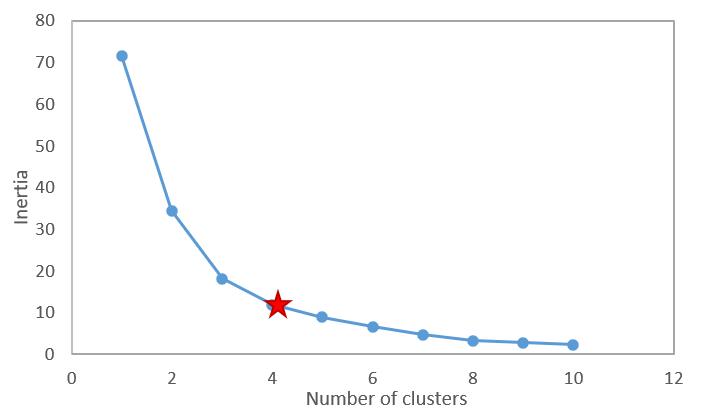
\includegraphics[width=7.5cm]{figure/肘部4}
    \caption{铅钡玻璃化学成分量化权重图}
    \label{zhou}
  \end{minipage}
  \begin{minipage}[t]{0.48\textwidth}
    \centering
    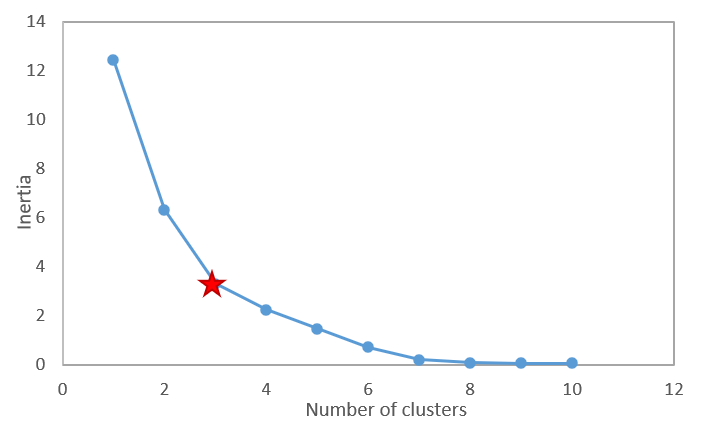
\includegraphics[width=7.5cm]{figure/肘部1}
    \caption{高钾玻璃化学成分量化权重图}
    \label{zb}
  \end{minipage}
\end{figure}

由图可见,对于铅钡玻璃,当类数从1增加到4时,总畸变程度下降较快;但当类别数超过4时,总畸变程度变化趋势变缓。对此,本文确定$k=4$为铅钡玻璃的最佳聚类数。同理确定$k=3$为高钾玻璃的最佳聚类数。铅钡玻璃主成分$r1$、$r2$按照$k=4$进行聚类后,聚类效果散点图展示如图\ref{km}。

\begin{figure}[H]
  \centering
  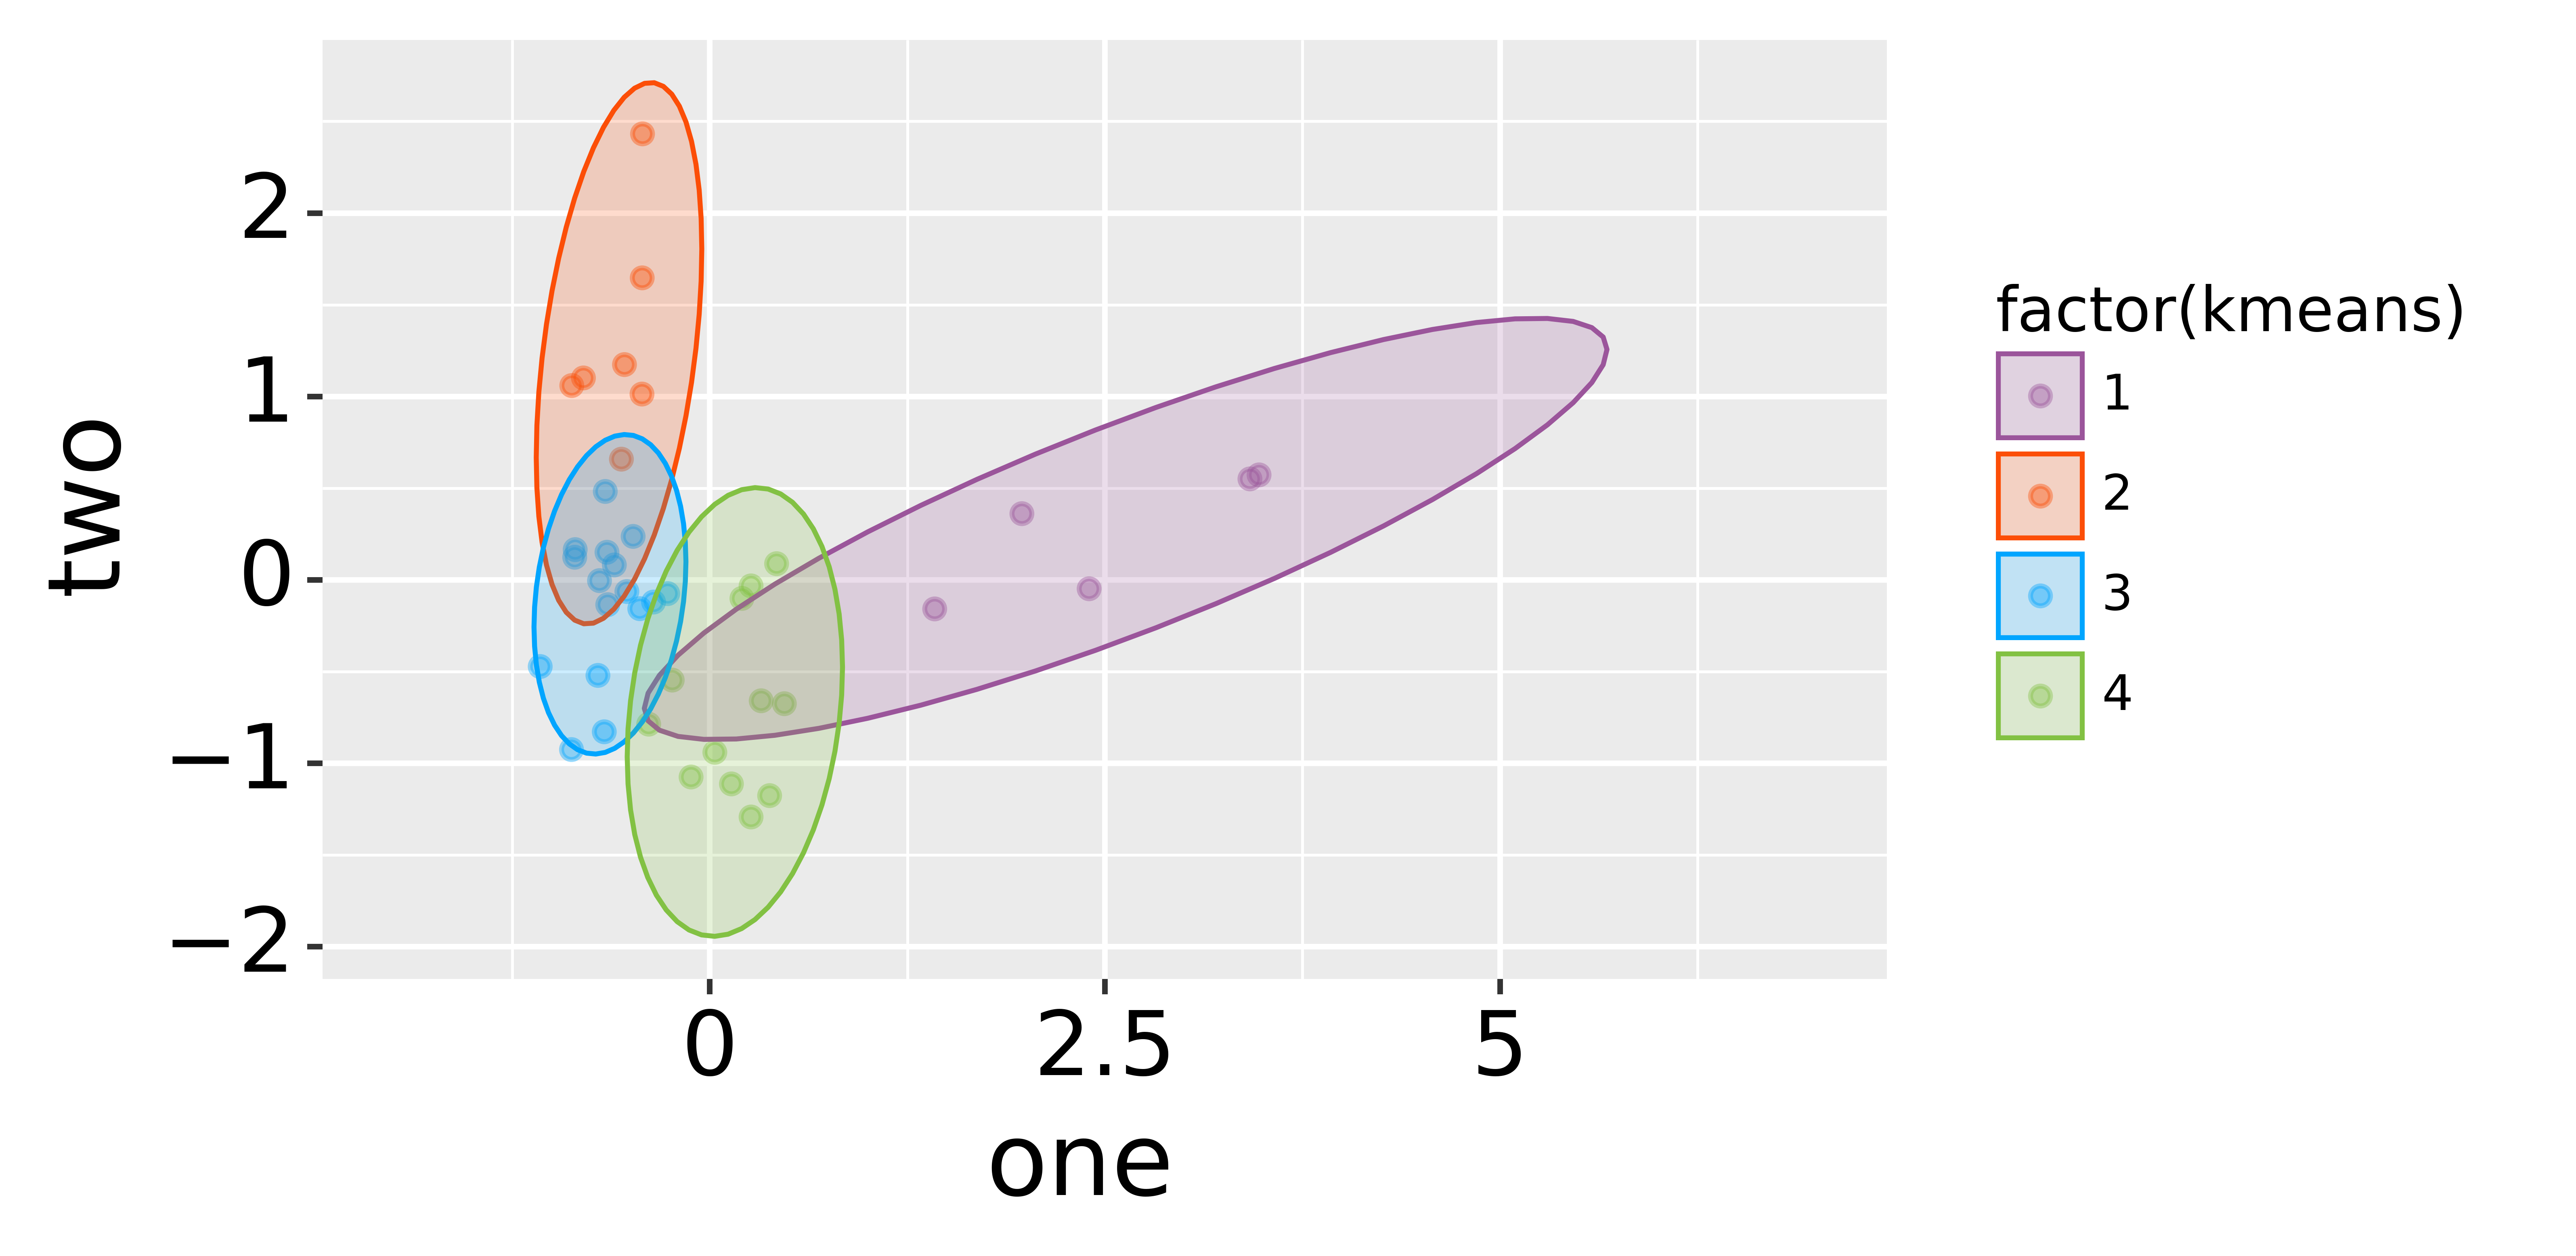
\includegraphics[width=0.8\textwidth]{figure/散点}
  \caption{铅钡玻璃聚类效果散点图}
  \label{km}
\end{figure}

基于K-Means++聚类得到铅钡玻璃的4种亚类划分以及对应化学成分含量的均值如下表:

\begin{table}[H]
  \centering
  \caption{铅钡玻璃亚类划分结果表}
  \begin{tabular}{ccccccc}
    \toprule[1.5pt]
    亚类          & 氧化钠均值    & 氧化铜均值    & 氧化铅均值    & 氧化钡均值    & 五氧化二磷均值  & 计数 \\ \hline
    1 & 0.02  & 7.83     & 17.15  & 25.57   & 3.26 & 5  \\
    2 & 3.99 & 1.12 & 16.82 & 9.04    & 0.02     & 7  \\
    3        & 0.62  & 0.57  & 25.93 & 6.44 & 0.49  & 16 \\
    4  & 0.28 & 1.6 & 26.58 & 8.89 & 3.31 & 12\\
    \bottomrule[1.5pt]
  \end{tabular}
\end{table}


结合上表中不同亚类下各项化学成分均值的大小关系,将铅钡玻璃的亚类1-4分别记为高$CuO$-中$PbO$-高$BaO$-高$P_2O_5$、高$Na_2O$-低$CuO$-中$PbO$-中$BaO$、高$PbO$-$BaO$、低$CuO$-高$PbO$-$BaO$-高$P_2O_5$。其中,高$PbO$-$BaO$亚类的数据量最大,说明铅钡玻璃中氧化铅含量较大的玻璃占该类玻璃的较大部分。该结果与分类规律分析中氧化铅含量对玻璃类型的显著影响的结果相互印证,体现了本文模型建立的连贯性与一致性。

\begin{table}[H]
  \centering
  \caption{高钾玻璃亚类划分结果表}
  \begin{tabular}{ccccccc}
    \toprule[1.5pt]
    亚类 & 氧化钠均值 & 氧化钡均值 & 氧化铜均值 & 氧化钙均值 & 氧化钾均值 & 计数 \\ \hline
    1  & 0.00  & 1.53  & 2.85  & 3.79  & 5.44  & 3  \\
    2  & 0.00  & 0.00  & 1.87  & 6.28  & 9.81  & 10 \\
    3  & 2.78  & 0.00  & 2.09  & 8.40  & 13.11 & 3  \\ \bottomrule[1.5pt]
  \end{tabular}
\end{table}

结合上表中不同亚类下各项化学成分均值的大小关系,将高钾玻璃的亚类1-3分别记为$BaO$-高$CuO$-低$CaO$-低$K_2O$、$CuO$-$CaO$-$K_2O$、$Na_2O$-$CuO$-高$CaO$-高$K_2O$。其中,$CuO$-$CaO$-$K_2O$亚类的数据量最大,说明高钾玻璃中氧化钙和氧化钾含量较大的玻璃占该类玻璃的较大部分。

基于上述不同玻璃类型下的亚类划分,得到古代玻璃制品的分类树如下图\ref{shu}:

\begin{figure}[H]
  \centering
  \includegraphics[width=1\textwidth]{figure/树}
  \caption{古代玻璃制品分类图}
  \label{shu}
\end{figure}

\subsection{合理性与敏感性分析}

\subsubsection{基于K-W检验与数据分布的合理性分析}

首先,本文利用Kruskal-Wallis(K-W)检验对聚类结果的合理性进行分析,即分析铅钡玻璃和高钾玻璃聚类所得数据在不同聚类簇中是否存在显著差异。检验结果如下表:
\begin{table}[H]
  \centering
  \caption{K-W检验结果表}
  \begin{tabular}{ccccccc}
    \toprule[1.5pt]
    \multicolumn{3}{c}{铅钡玻璃}      &  & \multicolumn{3}{c}{高钾玻璃}    \\ \cline{1-3} \cline{5-7} 
    分析项   & p值       & Cohen's f值 &  & 分析项 & p值       & Cohen's f值 \\ \hline
    氧化钠   & 0.000*** & 0.309      &  & 氧化钠 & 0.001*** & 0.635      \\
    氧化铜   & 0.000*** & 0.403      &  & 氧化钾 & 0.004*** & 0.521      \\
    氧化铅   & 0.006*** & 0.21       &  & 氧化钙 & 0.008*** & 0.395      \\
    氧化钡   & 0.002*** & 0.382      &  & 氧化铜 & 0.441    & 0.152      \\
    五氧化二磷 & 0.000*** & 0.278      &  & 氧化钡 & 0.001*** & 0.629      \\ \bottomrule[1.5pt]
  \end{tabular}
\end{table}

观察上表发现,铅钡玻璃下各项化学成分含量的检验结果$p$值为$0.000^{***}<0.05$,因此统计结果显著,说明各项化学成分含量在不同聚类簇上存在显著差异。高钾玻璃下氧化钠、氧化钾、氧化钙、氧化钡的检验结果$p$值为$0.000^{***}<0.05$,即上述化学成分含量在不同聚类簇上存在显著差异。而对于氧化铜含量,为表现出显著差异,本文判断是由于氧化铜为着色剂,在不同类别玻璃中的含量变化较小,因此显著性较差。综合分析,检验结果表面,本文针对铅钡玻璃与高钾玻璃进行的聚类具有较强的合理性,得到了有价值的亚类划分。

此外,本文利用所得亚类划分方式对表单2中原始数据,即风化与未风化化学成分含量数据进行亚类划分,得到风化与未风化情况下亚类划分结果的数据分布如下图\ref{jy}和图\ref{jyy}:

\begin{figure}[H]
  \centering
  \begin{minipage}[t]{0.48\textwidth}
    \centering
    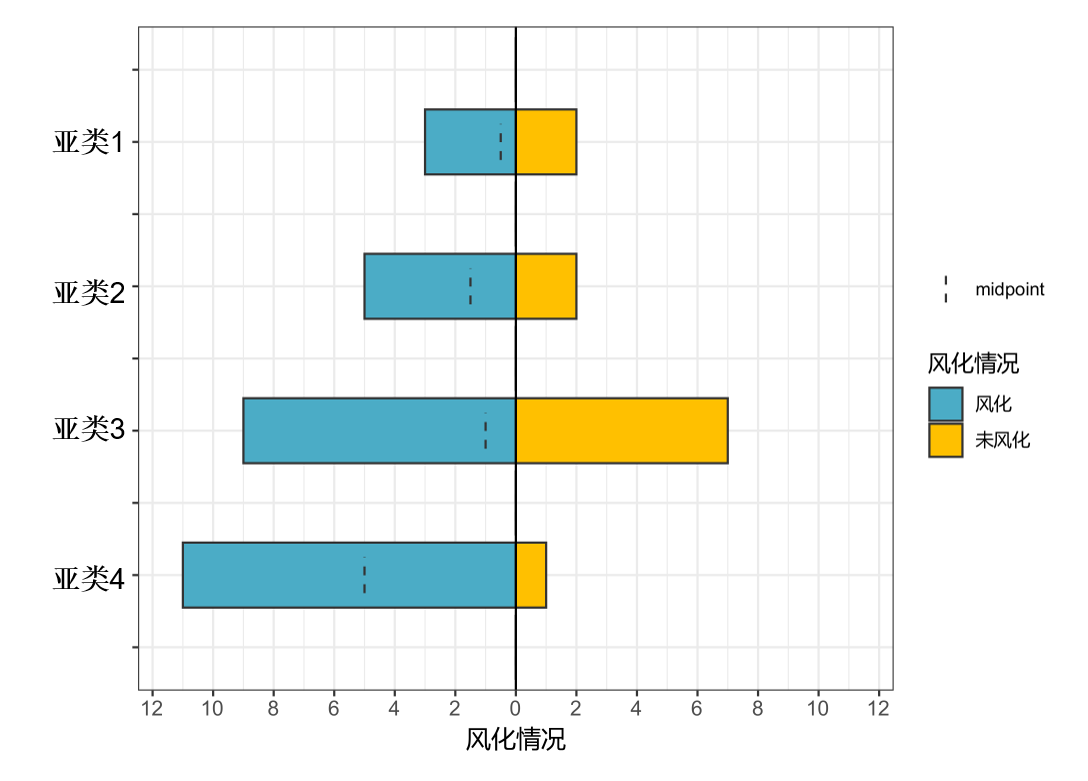
\includegraphics[width=7.5cm]{figure/检验2}
    \caption{铅钡玻璃有无风化数据亚类图}
    \label{jy}
  \end{minipage}
  \begin{minipage}[t]{0.48\textwidth}
    \centering
    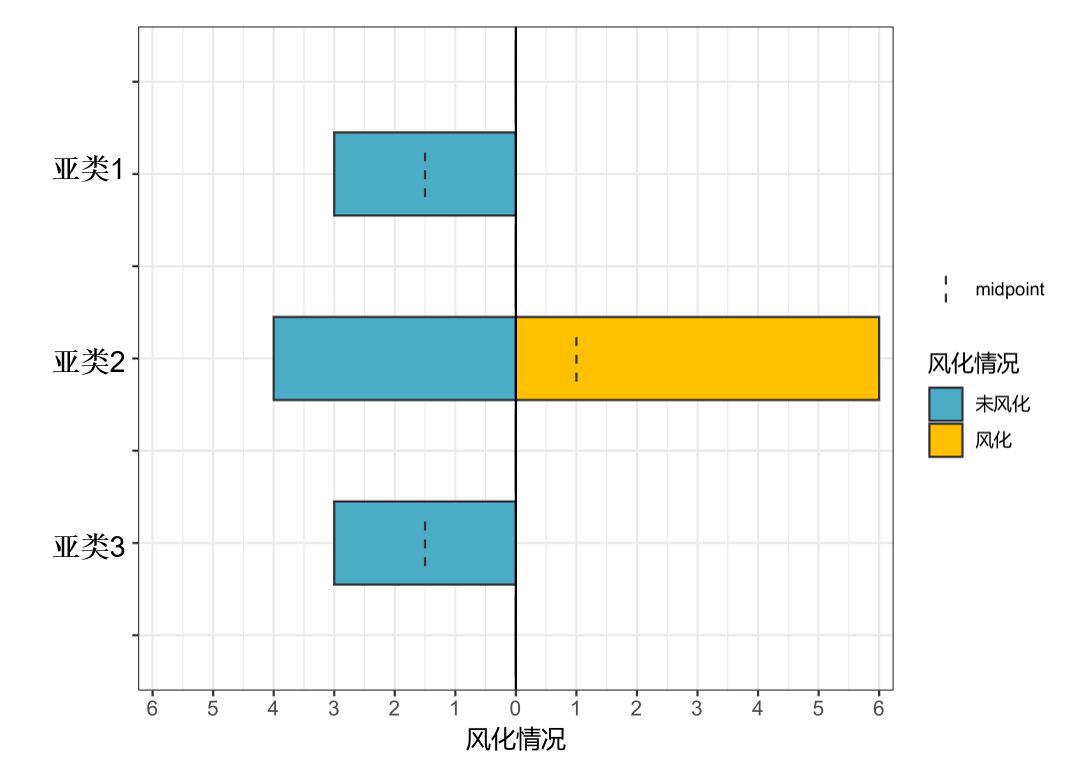
\includegraphics[width=7.5cm]{figure/检验1}
    \caption{高钾玻璃有无风化数据亚类图}
    \label{jyy}
  \end{minipage}
\end{figure}

由上图可知,对于铅钡玻璃中表面风化点的数据,在各亚类中的分布较为均匀,说明了本文选择分类数据的合理性,即将风化数据转化为未风化数据的数据处理行为是合理的。对于高钾玻璃中的表面风化点的数据,由于该数据本身并不含有化学成分氧化钠与氧化钡,则依据分类规则显然会被归于亚类2。而受到数据特征局限的分类结果仍在亚类2中表现出风化与未风化的均匀分布,再次印证了本文亚类划分的合理性。

\subsubsection{基于权重调节的敏感性分析}

本文针对不同类型的玻璃制品选择重要化学成分,通过调节该成分的量化权重分析不同情况下亚类划分的数据分布情况,分析亚类划分模型的敏感性。对于铅钡玻璃,本文选择量化权重较大且能体现该类玻璃特异性的化学成分氧化钠进行敏感性分析。对于高钾玻璃,本文选择氧化钾进行敏感性分析。此处以铅钡玻璃为例进行分析,高钾玻璃的相关结果见附录。调节氧化钠量化权重后的铅钡玻璃亚类数据分布如下图\ref{mg1}:
\begin{figure}[H]
  \centering
  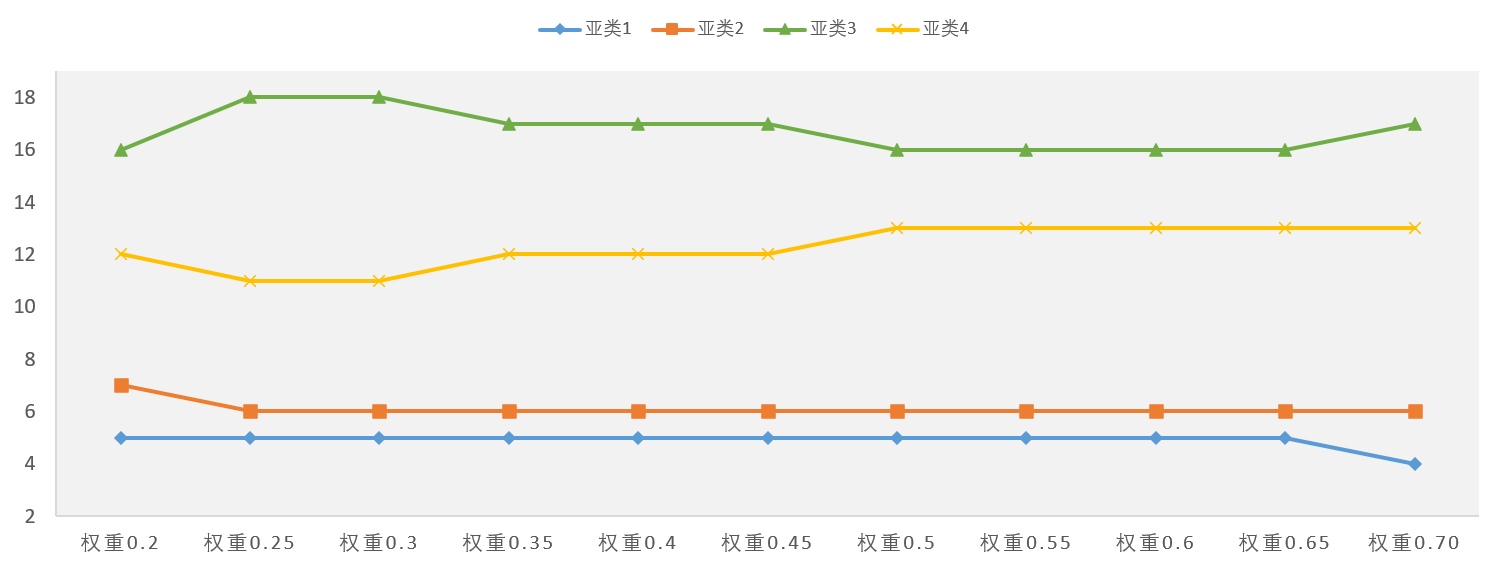
\includegraphics[width=1\textwidth]{figure/敏感1}
  \caption{基于氧化钠权重调节的铅钡玻璃敏感性分析图}
  \label{mg1}
\end{figure}

观察上图可知,亚类3高$PbO$-$BaO$与亚类4低$CuO$-高$PbO$-$BaO$-高$P_2O_5$对于氧化钠量化权重的变化较为敏感。本文判断是由于与高氧化钠含量的亚类2不同,亚类3与亚类4中氧化钠含量较低,因此氧化钠含量微小的变化也会对此类别造成较大影响。而对于氧化钠含量较高的亚类1和亚类2,氧化钠量化权重对类别分布的影响较小。综合分析,亚类划分对化学成分量化权重的敏感性体现出不同亚类上的差异性,并与该亚类的分类特征相适应。因此,敏感性分析的结果也从一定程度上印证了本文亚类划分的合理性。

\section{问题三的模型建立与求解}

\subsection{问题三的描述与分析}

问题三要求对表单3中文物的化学成分进行分析,判断各玻璃文物所属类别,并进行敏感性分析。首先,利用氧化铅对表单3中文物进行基类划分,即判断文物为铅钡玻璃与高钾玻璃。之后,利用回归方程将数据转化为风化前数据,并建立XGBoost分类模型对玻璃文物的亚类进行预测。其中,本文利用K折交叉验证与 贝叶斯调参对分类模型进行求解,以达到更好的预测效果。

\begin{figure}[H]
\centering
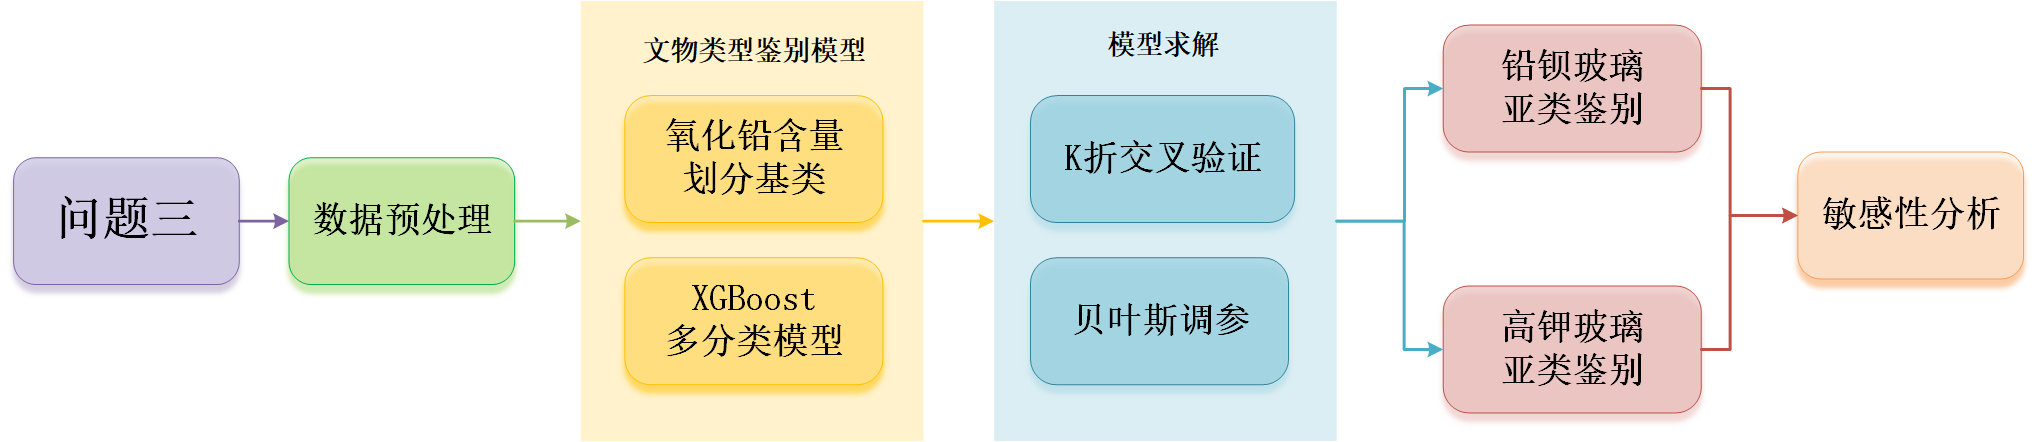
\includegraphics[width=1\textwidth]{figure/问题三}
\caption{问题三思路图}
\end{figure}

\subsection{数据预处理}

由于后续需基于问题二中分类结果对表单3中文物进行类型鉴别,本文利用\ref{jizhun}中各项化学成分的回归方程,将表单3中表面风化数据转化为风化前数据。

\subsection{基于XGBoost多分类的文物类型鉴别模型建立}

对于文物类型的鉴别,由于问题二中Logistic回归中氧化铅对基类准确划分,本文利用氧化铅对表单3中的文物进行初始基类划分,设表单3中第$i$个文物的氧化铅含量为$PbO_i$,该文物所属基类$L_i$满足:
\begin{equation}
  \begin{cases}
    {L_i \in Q} & {PbO_i \geq 9.3}\\ {L_i \in G} & {PbO_i < 9.3}
  \end{cases}
\end{equation}
其中,$Q$为铅钡玻璃,$G$为高钾玻璃。9.3即为问题二中分析所得氧化铅划分玻璃类型的临界含量。

之后,以表单2中数据作为XGBoost分类模型的训练集,对表单3中的文物数据进行分类。设第$i$个文物的14项化学成分指标分别为$x_{i,1},\cdots,x_{i,14}$,玻璃文物所属类型为$y_{i}$。XGBoost进行additive training,学习$K$棵树,采用以下函数对样本进行预测\textsuperscript{\cite{ref9}}:

\begin{equation}
  \tilde { y_{i} } =  \sum _ { k = 1 } ^ { K } f _ { k } ( x _ { i,j} ) ,\quad f _ { k } \in \Gamma;j=1,2,\cdots,14.
  \label{shi1}
\end{equation}
其中$f(x)$是分类树,$\Gamma$是假设空间:

\begin{equation}
  \Gamma = \{ f ( x ) = w _ { q ( x ) } \} ( q : R ^ { m } \rightarrow T , w \in R ^ { T } ).
  \label{shi2}
\end{equation}
其中,$q(x)$表示样本$x$分到了某个叶子节点上,$w$是叶子节点的分数,所以$w _ { q ( x ) }$表示分类树对文物所属亚类的预测值。


\subsection{模型求解}

\subsubsection{K折交叉验证}

在利用XGBoost分类模型对文物所属类别进行预测过程中,本文利用K折交叉验证进行数据集的划分与选择。K折交叉验证指的是将数据集划分为K等份,每次取其中一组数据作为测试集,其余数据作为训练集进行求解。该方法可以有效地防止过拟合的问题,并找到合适的模型参数。K折交叉验证示意图如下图\ref{kzhe}:

\begin{figure}[H]
  \centering
  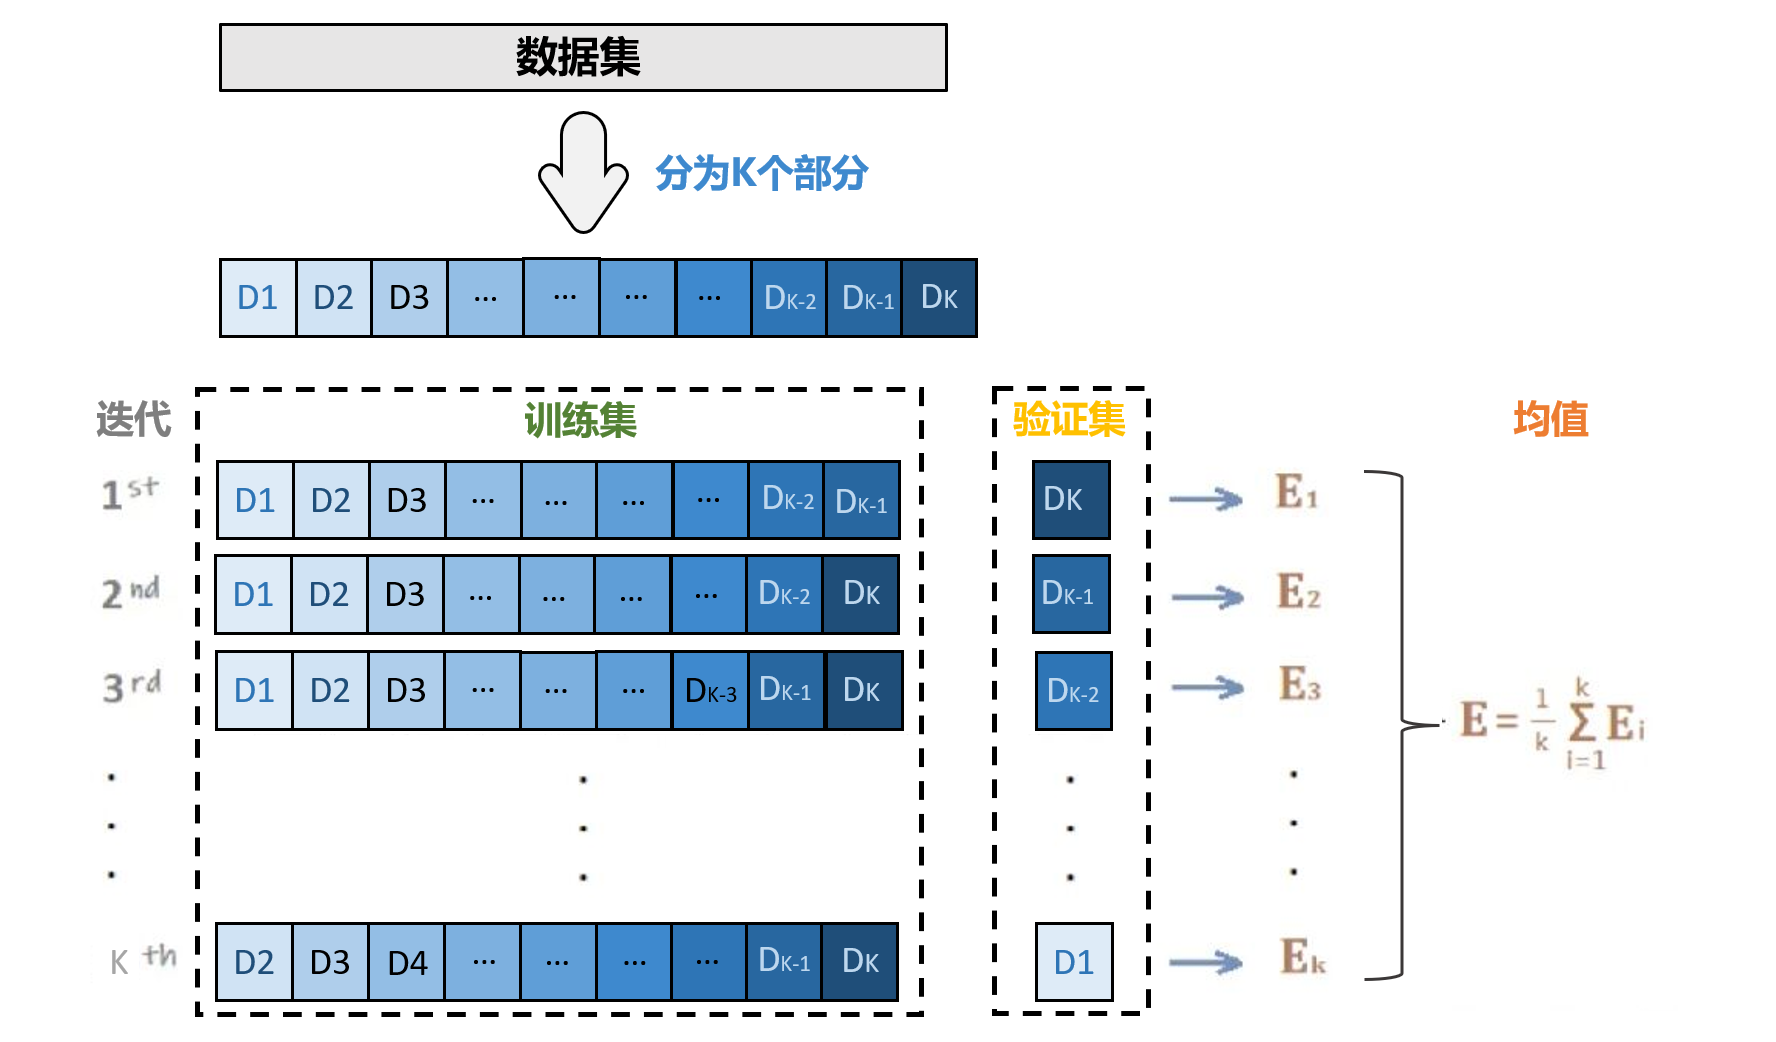
\includegraphics[width=0.9\textwidth]{figure/k折}
  \caption{K折交叉验证示意图}
  \label{kzhe}
\end{figure}

\subsubsection{贝叶斯调参}

在利用XGBoost进行分类的求解过程中,本文引入了贝叶斯调参进行模型参数的调节,从而达到更好的分类效果。其中,本文以交叉验证集F1分数最大为标准进行参数调节。贝叶斯调参流程的伪代码如下\textsuperscript{\cite{ref5}}:

\begin{algorithm}[H]
  \caption{ Sequential Model-Based Optimization}
  \begin{algorithmic}[1]
    \State \textbf{Input:} $f,X,S,M$
    
    \State D $\leftarrow$ $INITSAMPLES(f,X)$
    
    \For $i \leftarrow |D| $\textbf{to} $T$
    
    \State  $p(y|x,D) \leftarrow FITMODEL(M,D)$; $x_i \leftarrow arg \max_{x \in X} S(x,p(y|x,D))$
    
    \State   $y_i \leftarrow f(x_i)$ $\triangleright$ Expensive  step; $D \leftarrow D \cup (x_i,y_i)$
    \EndFor
  \end{algorithmic}
\end{algorithm}

\subsection{求解结果与分析}

本文建立XGBoost多分类模型对表单3中的文物进行类别划分,并利用CatBoost模型与随机森林模型进行预测,与XGBoost预测效果进行对比。因为各算法在高钾玻璃上的分类均为准确分类,所以利用铅钡玻璃上交叉验证集的F1分数作为比较指标。三种算法的预测效果如下表:

\begin{table}[H]
  \centering
  \caption{三种算法F1分数对比表}
  \begin{tabular}{cccc}
    \toprule[1.5pt]
    & XGBoost & CatBoost & 随机森林  \\ \hline
    F1分数 & 0.826   & 0.594    & 0.736 \\ \bottomrule[1.5pt]
  \end{tabular}
\end{table}

对比上表三种算法F1分数可知,XGBoost分类模型的F1分数大于CatBoost分类模型与随机森林分类模型,具有较好的预测效果。XGBoost分类模型F1分数0.826说明了预测效果的优越性以及本文选择分类模型的合理性。

利用XGBoost分类模型对表单3中玻璃文物的类型判断结果如下表:

\begin{table}[H]
  \centering
  \caption{玻璃文物分类结果表}
  \begin{tabular}{cccc}
    \toprule[1.5pt]
    文物编号 & 分类预测结果  & 文物编号 & 分类预测结果  \\ \hline
    A1   & 高钾玻璃亚类1 & A5   & 铅钡玻璃亚类3 \\
    A2   & 铅钡玻璃亚类4 & A6   & 高钾玻璃亚类1 \\
    A3   & 铅钡玻璃亚类4 & A7   & 高钾玻璃亚类2 \\
    A4   & 铅钡玻璃亚类4 & A8   & 铅钡玻璃亚类4 \\ \bottomrule[1.5pt]
  \end{tabular}
\end{table}

\subsection{敏感性分析}

本文调节不同类型玻璃下的主要影响成分,计算各文物所属类别的变化次数以及变化所需调节次数,对分类模型对不同化学成分的敏感性。不同玻璃类型下调节化学成分对应的变化次数以及变化所需调节次数结果见附录。本文基于变化次数与调节次数定义敏感系数$\theta$,满足下式:
\begin{equation}
 \theta = \frac{n_{change}}{n_{regulate}}.
\end{equation}
其中,$n_{change}$为调节化学成分含量后文物所属类别的变化次数,$n_{regulate}$为变化所需调节次数。则敏感系数越大,分类模型对该成份变化的敏感性越大。

对于敏感系数为0即表现不敏感的化学成分不予展示,铅钡玻璃和高钾玻璃对应的不同化学成分含量的敏感系数如下表:

\begin{table}[H]
  \centering
  \caption{不同种类玻璃下化学成分的敏感系数表}
  \begin{tabular}{cclcc}
    \toprule[1.5pt]
    \multicolumn{2}{c}{铅钡玻璃} &  & \multicolumn{2}{c}{高钾玻璃} \\ \hline
    氧化钠       & 0.642857     &  & 氧化钠         & 0.5        \\
    氧化铅       & 0.438095     &  & 氧化钾         & 6          \\
    五氧化二磷     & 0.333333     &  &             &            \\ \bottomrule[1.5pt]
  \end{tabular}
\end{table}

由上图可知,铅钡玻璃的亚分类结果对氧化钠含量的变化最敏感,高钾玻璃的亚分类结果对氧化钾含量的变化最敏感。该结果与问题二中分析所得的主要影响指标相互印证,说明了本文模型建立的合理性与前后一致性。

\section{问题四的模型建立与求解}

\subsection{问题四的描述与分析}

问题四要求分析玻璃文物化学成分间的关联,并对不同类别下的关联关系的差异性进行比较。本文分别从宏观和微观层面对关联关系以及差异性进行分析。对于宏观层面分析,本文利用Kendall's W检验分析关联关系的显著性,利用配对t检验分析关联关系的差异性。对于微观层面分析,本文建立灰色关联量化模型,对化学成分间的关联关系以及不同类别玻璃下关联关系的差异性进行量化分析。得到对于铅钡玻璃,与其他化学成分关联强度最大的化学成分为氧化镁,对于高钾玻璃为氧化钙。二氧化硅与其他化学成分间的关联关系在不同种类的玻璃中体现出最大的差异性。

\begin{figure}[H]
\centering
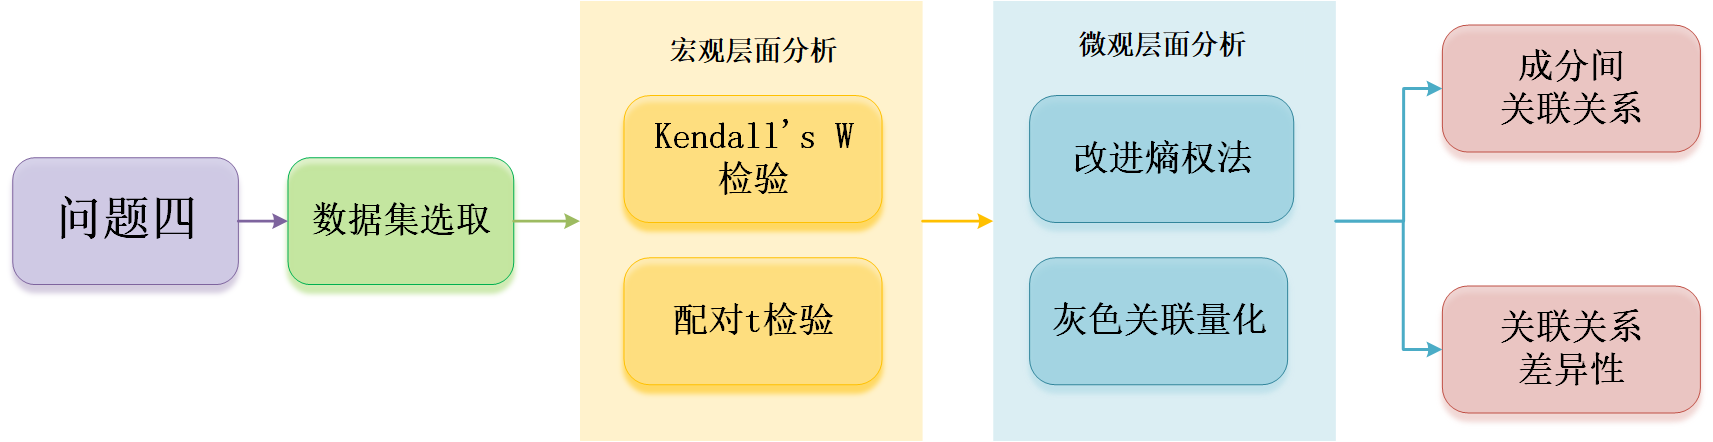
\includegraphics[width=0.9\textwidth]{figure/问题四}
\caption{问题四思路图}
\end{figure}

\subsection{数据集的选取}

由于亚分类下部分类别数据量极小,不具有分析关联性的价值,本文针对玻璃的基类进行关联性分析,即分析铅钡玻璃与高钾玻璃下不同化学成分含量的差异性。又由于表单3中基于氧化铅含量得到了准确基类划分结果,本文选取表单2和表单3中的数据进行后续分析。

\subsection{关联关系及差异性的宏微观分析模型建立}

本文分别从宏观和微观的角度对两类玻璃文物化学成分含量的关联性,以及不同类型玻璃对应的关联关系的差异性进行分析。

\subsubsection{基于Kendall's W检验与配对t检验的宏观层面分析}

首先,本文利用Kendall's W检验对两种类型玻璃下化学成分关联关系的显著性进行分析。以铅钡玻璃为例,检验原假设为铅钡玻璃下各项化学成分含量数据相互独立。计算检验统计量$p$值,并结合显著性水平$\alpha$进行分析。

之后,由于数据不符合正态分布,针对不同类型玻璃分别计算各项化学成分指标间的Spearman相关系数,满足下式:
\begin{equation}
 \rho=\frac{\sum_{i}\left(s_{i}-\bar{s}\right)\left(t_{i}-\bar{t}\right)}{\sqrt{\sum_{i}\left(s_{i}-\bar{s}\right)^{2} \sum_{i}\left(t_{i}-\bar{t}\right)^{2}}} .
\end{equation}
其中,$s_i$和$t_i$分别为计算相关系数的两项化学成分含量,$\bar{s}$和$\bar{t}$分别为该化学成分含量数据的均值。

由此,利用计算所得Spearman相关系数进行配对t检验,分析同一化学成分在不同类型玻璃中与其余13项化学成分的相关系数间是否存在显著差异,即分析不同玻璃下化学成分含量关联的差异性。以二氧化硅指标为例,检验原假设为二氧化硅含量与其余13项化学成分含量的相关系数在铅钡玻璃与高钾玻璃中相互独立。计算检验统计量$p$值,并结合显著性水平$\alpha$进行分析。

\subsubsection{基于灰色关联量化模型的微观层面分析}

本文利用灰色关联量化模型对同种类型玻璃下各化学成分与其他成分间的关联程度进行量化,从而量化地分析各化学成分间的关联关系\textsuperscript{\cite{ref10}}。同样,本文利用灰色关联量化模型对不同玻璃下关联关系的差异性进行量化,从而量化地分析不同类别玻璃之间化学成分关联关系的差异性。


\begin{itemize}
  \item \textbf{量化指标选取}
\end{itemize}

对于化学成分关联关系的分析,本文选取化学成分间相关系数的绝对值作为量化指标,衡量化学成分间的关联性强弱。对于不同种类玻璃化学成分关联关系的差异性分析,本文选择两种类型玻璃各化学成分间的相关系数之差的绝对值作为量化指标,衡量不同类型玻璃下化学成分关联关系的差异性\textsuperscript{\cite{ref10}}。

\begin{itemize}
  \item \textbf{改进的熵权法为量化指标赋权}
\end{itemize}

传统熵权法在所有熵值趋近于1时,会过度放大权重差距,赋权不合理。由于指标差距越小权重越大,本文对熵权法中的权重计算进行改进,从而克服传统赋权确定的不合理性。以铅钡玻璃下化学成分关联关系的分析为例,赋权步骤如下:

\textbf{Step1:建立初始量化矩阵和指标数据标准化。} 针对不同化学成分的关联程度量化,我们有14个量化方案,即14种不同化学成分指标,13个量化指标,即该化学成分与其余13项化学成分间的Spearman相关系数绝对值。设$m_{i,j}(i=1,2,\cdots,14;j=1,2,\cdots,13)$是第$i$个方案中第$j$个量化指标,则初始量化矩阵为$M=(m_{i,j})_{14 \times 13}$

\textbf{Step2:计算各项指标的信息熵。}第$j$项指标的信息熵$z _ { j }$为:

\begin{equation}
  z _ { j } = - \frac { 1 } { \ln 14 } \sum _ { i = 1 } ^ { 14 } l _ { i,j } \ln l _ { i,j }.
\end{equation}
其中,$l_{i,j}$为第$j$项指标下第$i$个方案占该指标的比重。

\textbf{Step3:确定各指标权重。} 第$j$项指标的权重为:
\begin{equation}
  o _ { j } = \left\{ \begin{array} { l r } { ( 1 - \overline { z_j } ^ { \alpha } ) o _ {  j } + \overline { z_j } ^ { \alpha }\overline{ o _ {  j } },}&{ z _ { j } < 1 } \\ { 0 , } & { z _ { j } = 1 } \end{array} \right. .
\end{equation}
其中,$\overline{o_{j}}$为指标$m_j$的平均权重,$z_j$为对应的熵值,$\overline { z_j }$为全部不为1的熵权的平均值,$\alpha$为熵值指数,一般取量化方案的个数。

\begin{itemize}
  \item \textbf{灰色关联度模型量化关联程度}
\end{itemize}

灰色关联分析通常用于分析各个因素对结果的影响程度,本文利用灰色关联度模型对化学成分关联关系以及关联差异性进行量化分析。根据灰色关联决策的理论,以量化方案指标向量与相对最优方案指标向量的关联度作为量化方案优劣的准则。

相对最优方案均为每个指标的最小值$m_0 = (f_{0,1},f_{0,2},\cdots,f_{0,13})$,量化方案$h_i$的量化指标$m_j$与相对最优方案的量化指标间的灰色关联度$\gamma_i$为:

\begin{equation}
  \gamma _ { i  } = \frac { \xi \operatorname { max }  | f _ { i j } - 1 | } { | f _ { i j } - 1 | + \xi \operatorname { max } | f _ { i j } - 1 | }.
\end{equation}
其中,$\xi \in ( 0.1 )$为分辨系数,一般取作0.5。

由此可得到灰色关联度矩阵,并得到铅钡玻璃下14种化学成分的关联程度量化结果。对于高钾玻璃的关联关系以及两种玻璃下化学成分关联差异性的量化过程,与上述赋权以及关联度量化方法相同。

\subsection{模型求解与结果分析}

\subsubsection{宏观层面分析}

首先,本文对两种类型玻璃下化学成分的关联关系分别进行Kendall's W检验,检验结果如下表:

\begin{table}[H]
  \centering
  \caption{Kendall's W检验结果表}
  \begin{tabular}{cccc}
    \toprule[1.5pt]
    & Kendall's W系数 & $\chi^2$      & $p$       \\ \hline
    铅钡玻璃 & 0.754         & 391.916 & 0.000*** \\
    高钾玻璃 & 0.806         & 167.577 & 0.000*** \\ \bottomrule[1.5pt]
  \end{tabular}
\end{table}

由上表可知,铅钡玻璃和高钾玻璃下各项化学成分含量关联关系的检验结果$p$值均为$0.000*** < 0.05$,拒绝原假设。因此,两种类型玻璃下的各项化学成分间整体表现为显著相关。由此可知对化学成分含量间关联关系的进一步微观分析是必要的。

之后,本文对两种类型玻璃下的各项化学成分分别计算Spearman相关系数,铅钡玻璃和高钾玻璃化学成分的关联关系分别展示如下图\ref{xiantu}和图\ref{xt}:

\begin{figure}[H]
  \centering
  \begin{minipage}[t]{0.48\textwidth}
    \centering
    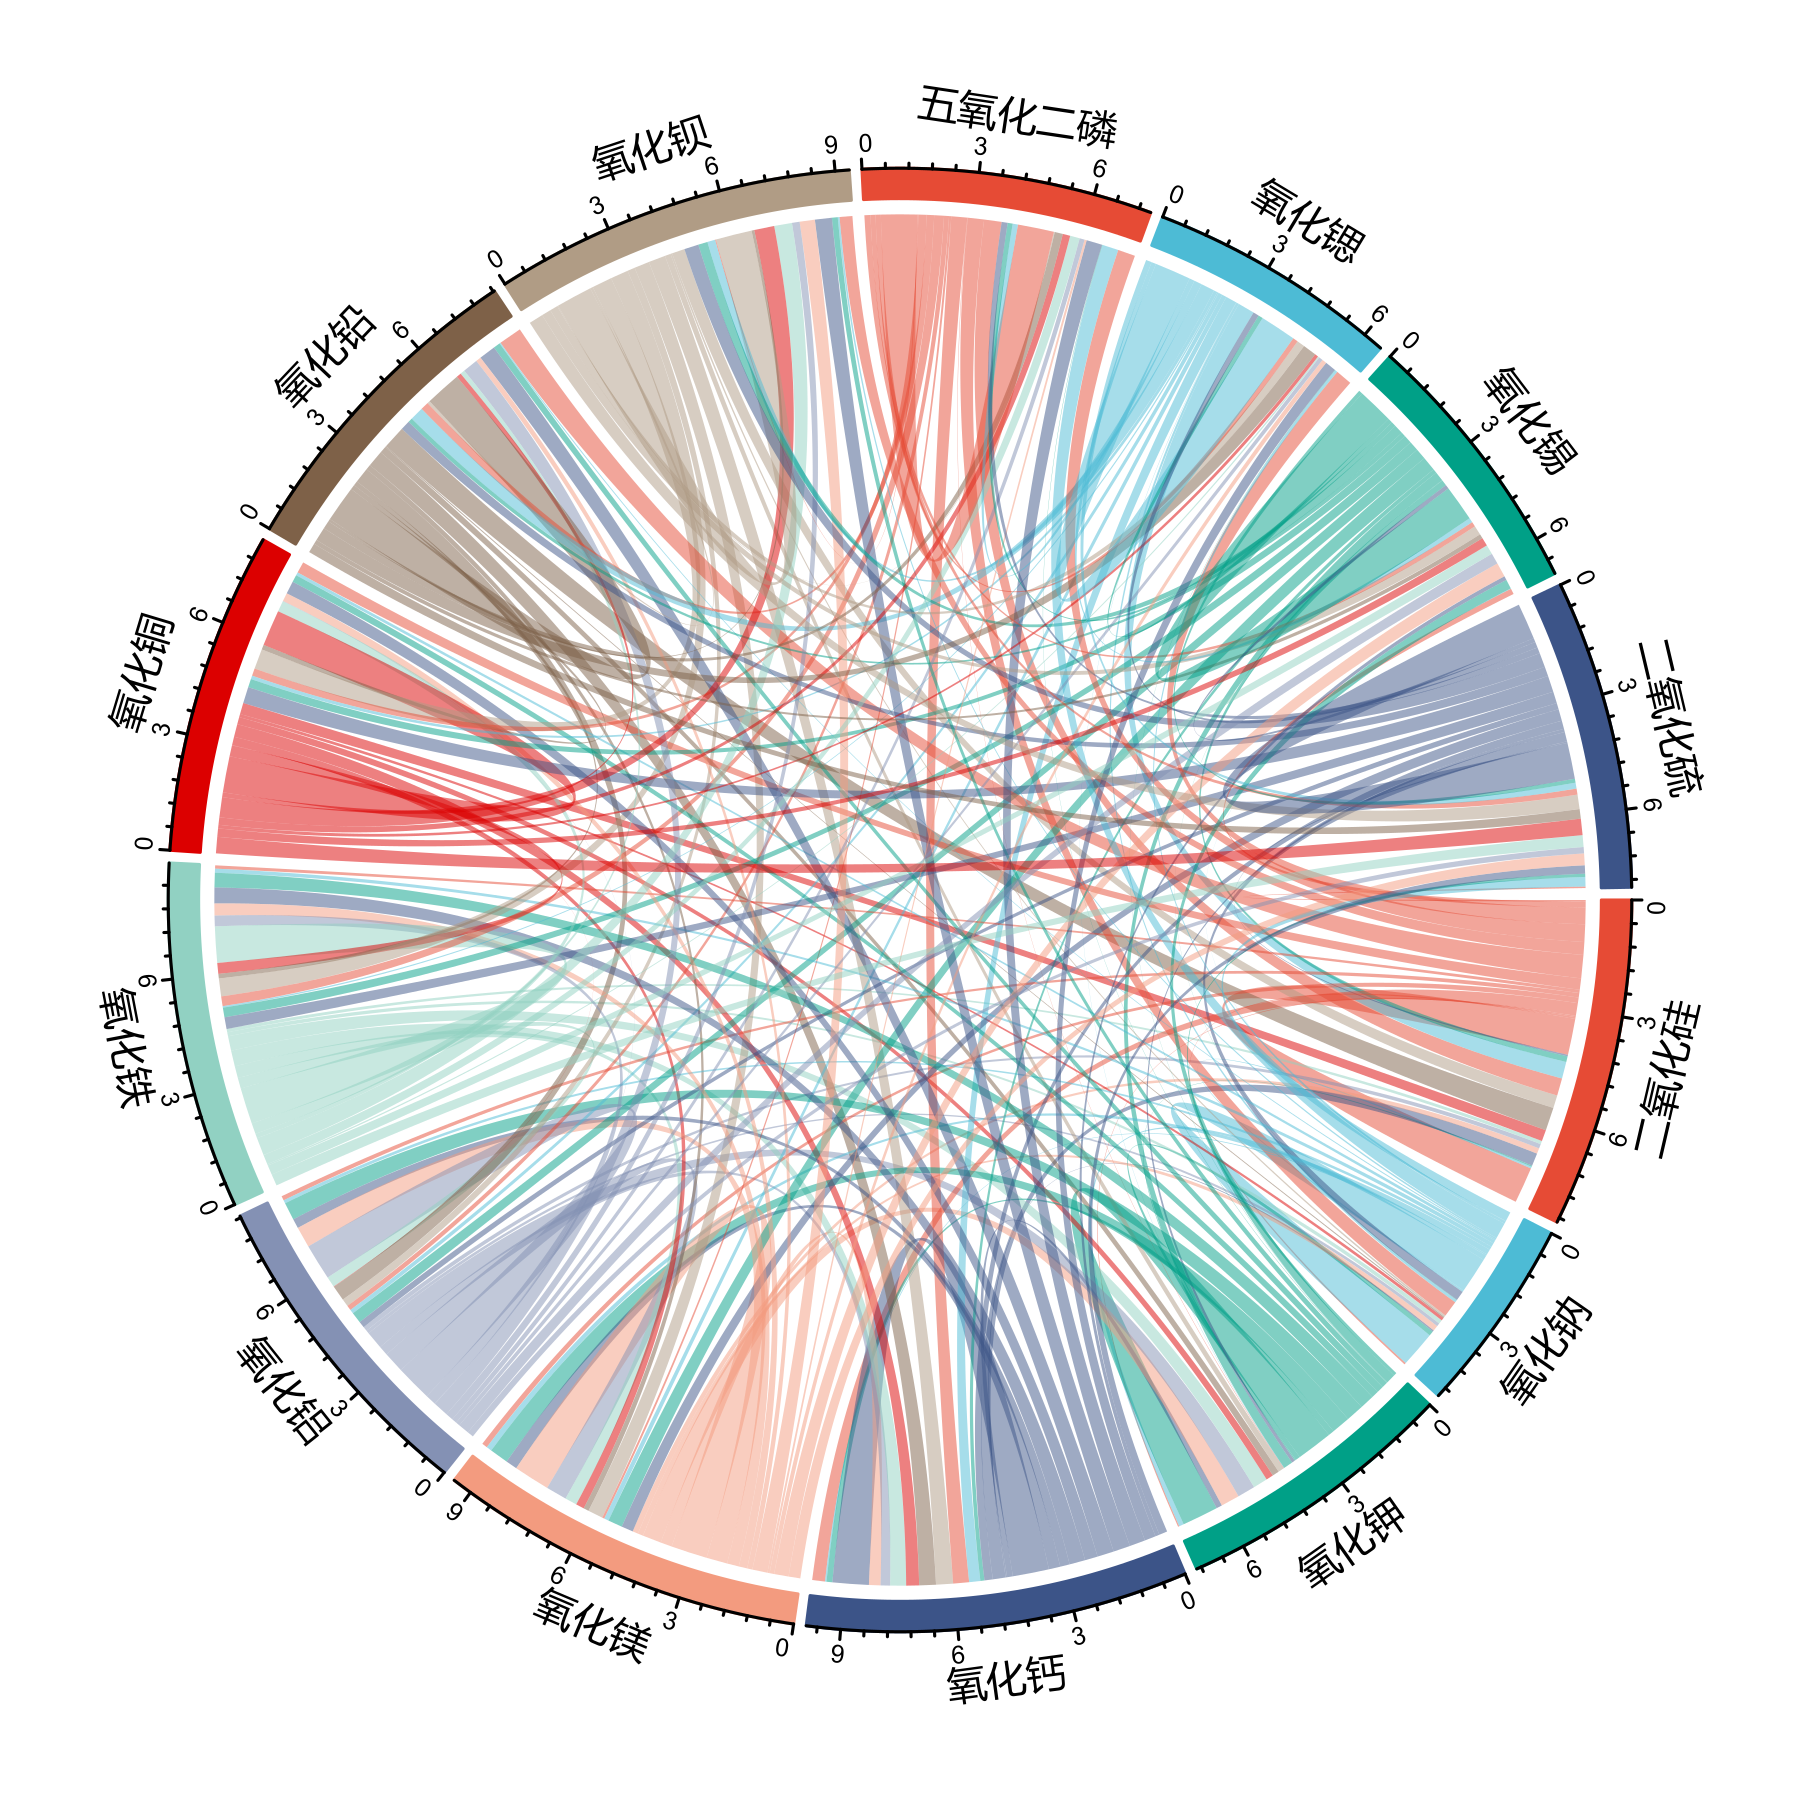
\includegraphics[width=6.5cm]{figure/铅弦图}
    \caption{铅钡玻璃化学成分关联图}
    \label{xiantu}
  \end{minipage}
  \begin{minipage}[t]{0.48\textwidth}
    \centering
    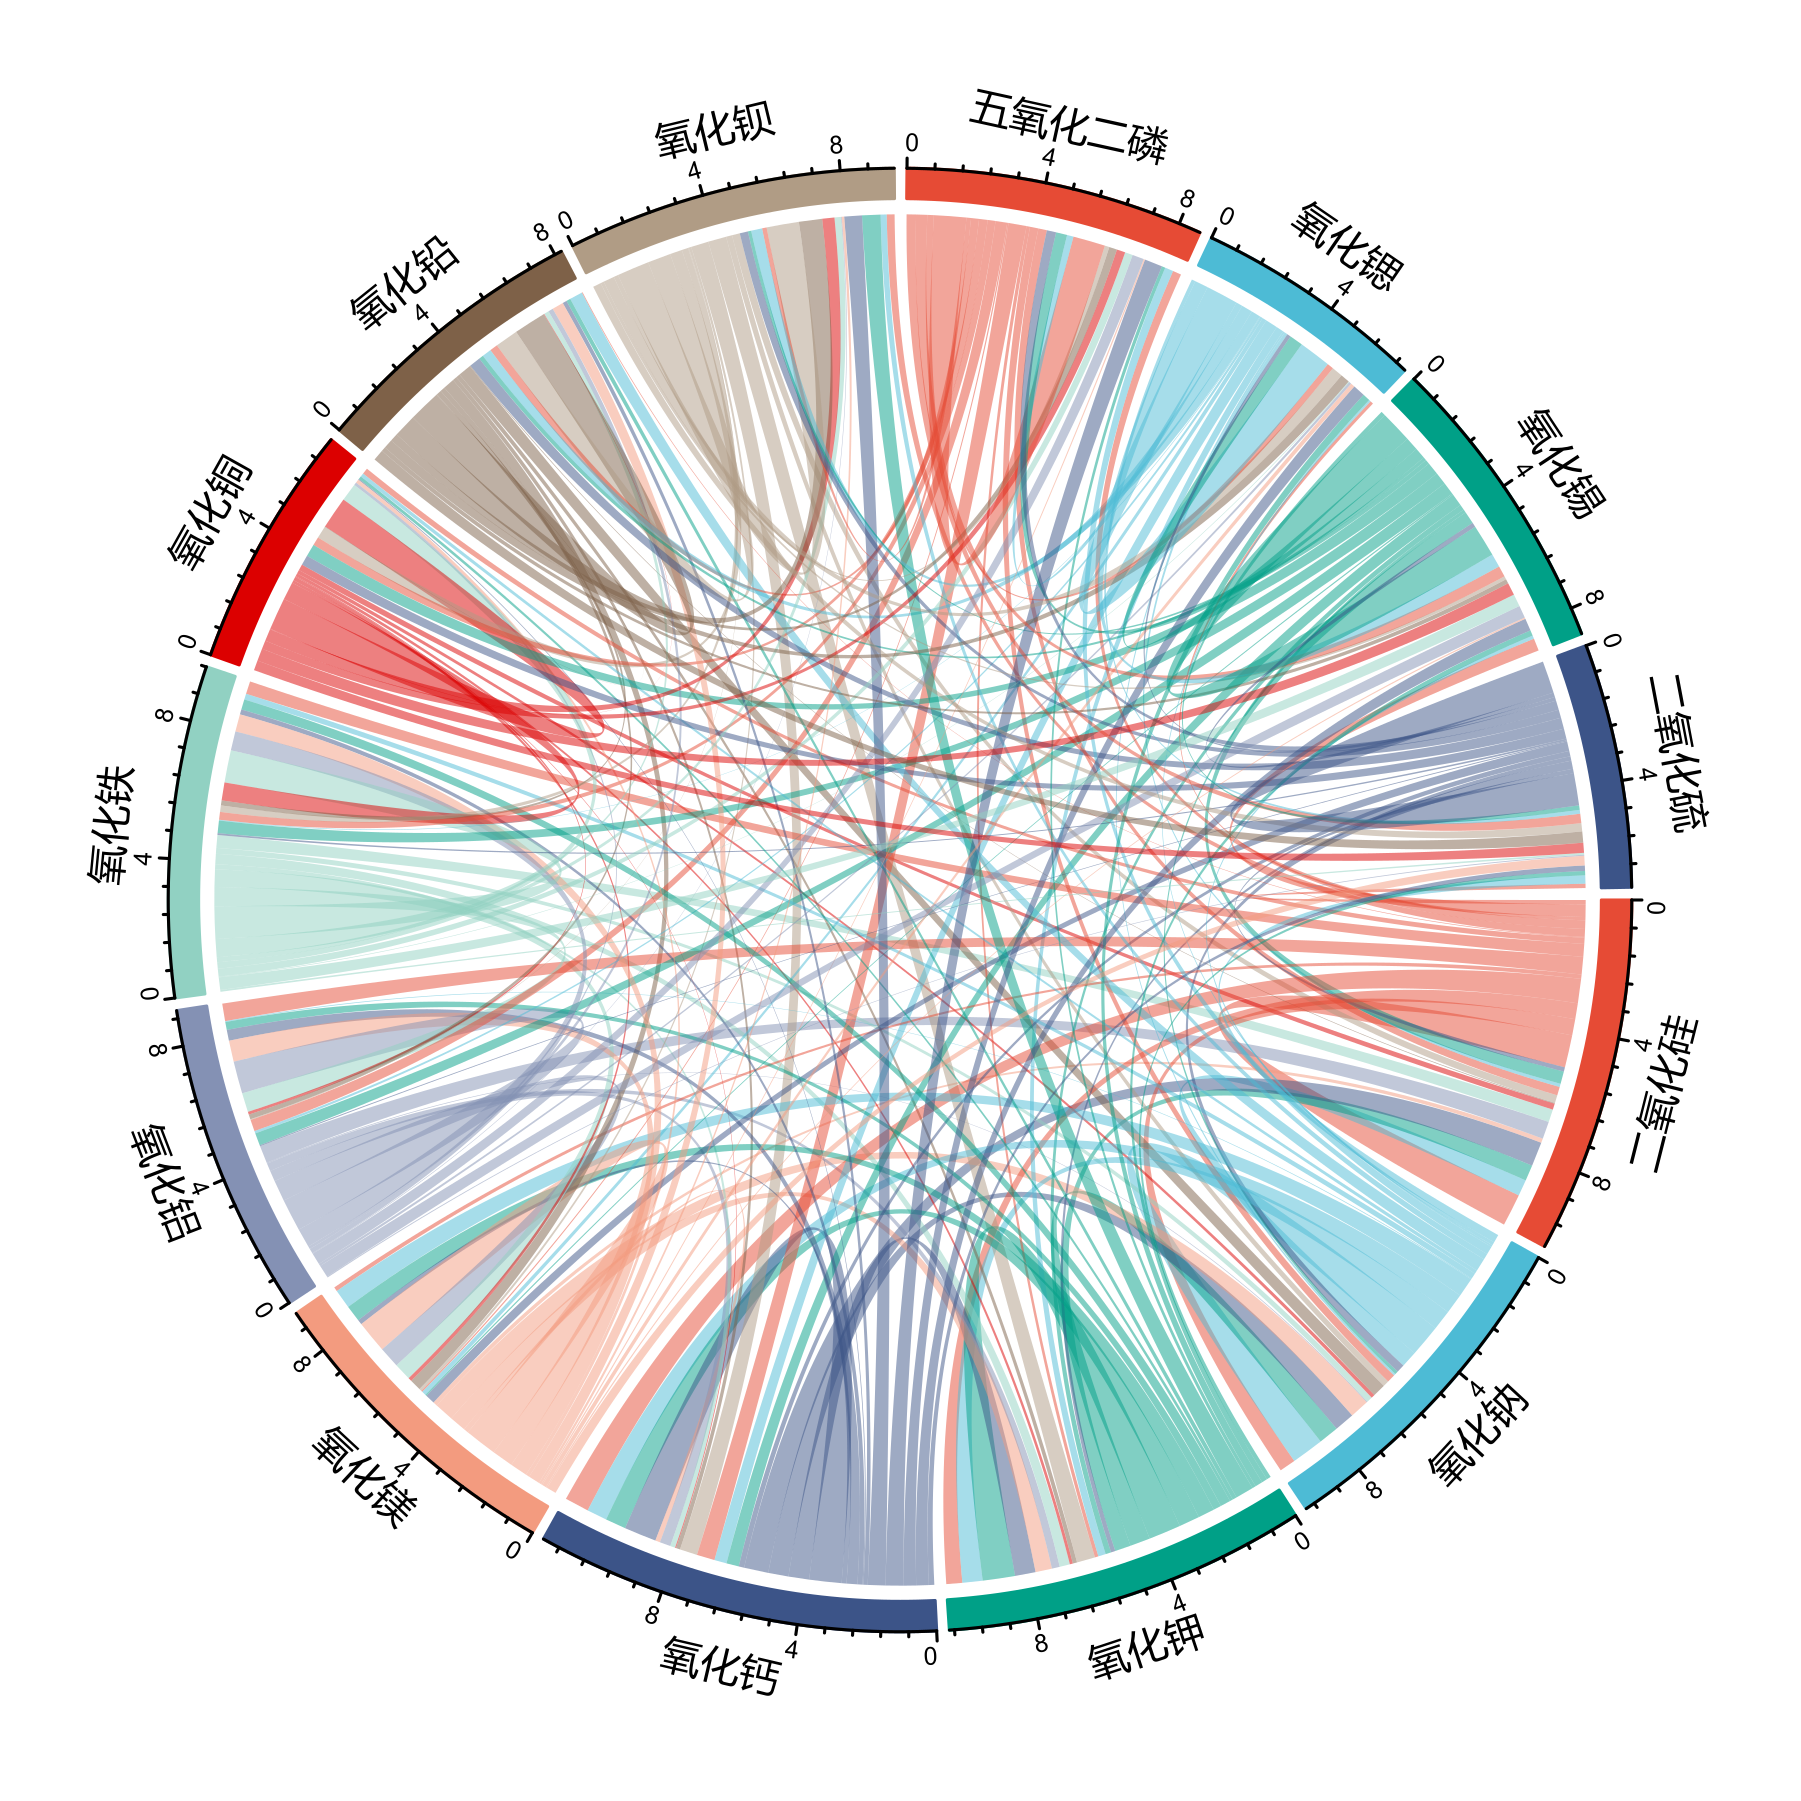
\includegraphics[width=6.5cm]{figure/钾弦图}
    \caption{高钾玻璃化学成分关联图}
    \label{xt}
  \end{minipage}
\end{figure}

由上图可知,部分化学成分关联关系在不同玻璃中表现出一致性,如二氧化硅与氧化钙在铅钡玻璃与高钾玻璃中的关联性均较大。而部分化学成分的关联关系在不同玻璃中表现出较大的差异性,如二氧化硅与氧化锶在铅钡玻璃中的关联性较大,而在高钾玻璃中关联性很小。因此,需对不同类型玻璃中同组化学成分间的关联关系的差异性进行进一步分析\textsuperscript{\cite{ref11}}。

本文利用配对t检验,对不同玻璃下同一化学成分与其余化学成分间相关系数的差异性进行分析。检验结果如下表:

\begin{table}[H]
  \centering
  \caption{配对t检验结果表}
  \begin{tabular}{cccccccc}
    \toprule[1.5pt]
    化学成分 & T值     & P值    & Cohen's d & 化学成分  & T值     & P值    & Cohen's d \\ \hline
    二氧化硅 & -0.281 & 0.784 & 0.078     & 氧化铜   & 1.595  & 0.137 & 0.442     \\
    氧化钠  & -0.012 & 0.99  & 0.003     & 氧化铅   & 0.415  & 0.685 & 0.115     \\
    氧化钾  & -1.013 & 0.331 & 0.281     & 氧化钡   & 1.064  & 0.308 & 0.295     \\
    氧化钙  & -1.355 & 0.2   & 0.376     & 五氧化二磷 & -0.341 & 0.739 & 0.095     \\
    氧化镁  & -0.863 & 0.405 & 0.239     & 氧化锶   & -0.027 & 0.979 & 0.007     \\
    氧化铝  & -0.754 & 0.465 & 0.209     & 氧化锡   & -1.236 & 0.24  & 0.343     \\
    氧化铁  & 0.236  & 0.817 & 0.065     & 二氧化硫  & 0.799  & 0.44  & 0.222     \\ \bottomrule[1.5pt]
  \end{tabular}
\end{table}

观察上表的检验结果发现,化学成分间的关联关系在不同玻璃并未表现出较大差异。对于不同种类的玻璃,其成分中均含有助熔剂、着色剂等元素,不同化学成分的作用各有不同但在不同玻璃中表现出一致性。该结果说明了后续针对化学成分内部联系的微观分析是必要的。

\subsubsection{微观层面分析}


本文利用灰色关联量化模型对铅钡玻璃和高钾玻璃中各项化学成分的关联强度进行量化,铅钡玻璃和高钾玻璃量化结果如下图\ref{fen}和图\ref{f}:


\begin{figure}[H]
  \centering
  \begin{minipage}[t]{0.48\textwidth}
    \centering
    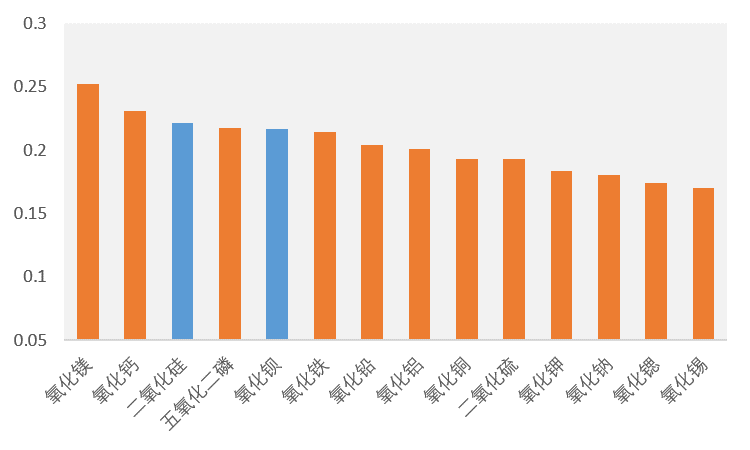
\includegraphics[width=7.5cm]{figure/铅得分}
    \caption{铅钡玻璃化学成分关联量化图}
    \label{fen}
  \end{minipage}
  \begin{minipage}[t]{0.48\textwidth}
    \centering
    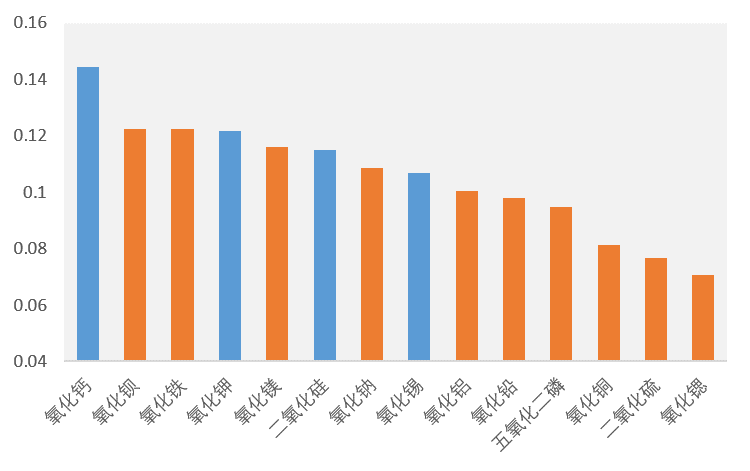
\includegraphics[width=7.5cm]{figure/钾得分}
    \caption{高钾玻璃化学成分关联量化图}
    \label{f}
  \end{minipage}
\end{figure}

上图中红色图形表示该化学成分与其他各项化学成分的关联关系大部分呈现出正向相关,蓝色图形表示该化学成分与其他各项化学成分的关联关系大部分呈现出负向相关。对于铅钡玻璃,与其他化学成分关联强度最大的化学成分为氧化镁,且大部分表现为正向相关。对于高钾玻璃,与其他化学成分关联强度最大的化学成分为氧化钙,且大部分表现为负向相关。

利用灰色关联量化模型对不同玻璃类型下关联关系的差异性进行量化,即以Spearman相关系数差的绝对值为量化指标得到的差异性量化结果如下表:

\begin{table}[H]
  \centering
  \caption{不同类型玻璃下化学成分关联关系的差异性量化结果表}
  \begin{tabular}{cccc}
    \toprule[1.5pt]
    化学成分 & 量化结果     & 化学成分  & 量化结果     \\ \hline
    二氧化硅 & 0.297662 & 氧化铜   & 0.1166   \\
    氧化钠  & 0.143264 & 氧化铅   & 0.190004 \\
    氧化钾  & 0.27256  & 氧化钡   & 0.223727 \\
    氧化钙  & 0.29736  & 五氧化二磷 & 0.155606 \\
    氧化镁  & 0.233788 & 氧化锶   & 0.10617  \\
    氧化铝  & 0.191022 & 氧化锡   & 0.213594 \\
    氧化铁  & 0.232116 & 二氧化硫  & 0.114032 \\ \bottomrule[1.5pt]
  \end{tabular}
\end{table}

观察上表可知,二氧化硅指标与其他化学成分间的关联关系在铅钡玻璃和高钾玻璃中体现出最大的差异性。

\section{模型评价}
\subsection{模型总结}

本文通过卡方检验对表单1中的定类数据进行关联分析,从三个维度对化学成分与表面是否风化的关系进行诠释,之后建立基于基准匹配策略的偏最小二乘回归模型对风化前的数据进行预测。对于不同玻璃类型的化学成分,利用Mann-Whitney检验和Logistic回归得到主要分类成分,之后建立基于量化权重的K-Means++聚类模型,对亚类进行划分。结合针对表单3的预测数据建立XGBoost多分类模型对数据进行亚类划分。建立灰色关联量化模型得到不同类型玻璃内部的关联关系和类型之间的关联关系的差异性。

\subsection{模型优缺点分析}
优点:

(1)第一问从三个维度对风化前后的化学成分数据进行分析与探讨, 使问题的分析更全面,结果更完善;

(2)创新性地利用统计规律建立基于基准匹配策略的偏最小二乘回归预测模型,得到较好的预测对象,使结果更加精确可信;

(3)第二问利用熵值和均值乘数得到化学成分的量化权重,并利用权重改进K-means++算法,得到更为合理的亚分类结果;

(4)第三问利用K折交叉验证和贝叶斯调参改进XGBoost的预测效果,使预测的结果更加精确;


(5)第四问从宏微观的角度分析成分间的关联关系和差异性,并从微观角度引入灰色关联量化模型得到较好的关联性量化结果。

缺点:

(1)基准匹配策略仅对数据的偏差进行求和,计算规则较为简单;

(2)化学成分之间的关联关系仅对不同玻璃类型的成分进行讨论,并没有对亚类的关联性进行探讨。

\subsection{模型改进与展望}
首先,本文利用基准匹配策略找到最佳的未风化数据匹配点,但距离的计算规则较为简单,可以后期引入迁移学习的思想对匹配策略进行更深的研究。化学成分的关联性可以结合亚类并利用成分同时出现的次数对关联性进行探讨和分析。

\newpage

\begin{thebibliography}{100}

\bibitem{ref6} Bailly Alexandre,Blanc Corentin,Roy Pascal. Effects of dataset size and interactions on the prediction performance of logistic regression and deep learning models[J]. Computer Methods and Programs in Biomedicine,2022,2(13):1-7.
\bibitem{ref2}Liu Jiamin,Ma Shuangge,Xu Wangli,Zhu Liping. A generalized Wilcoxon–Mann–Whitney type test for multivariate data through pairwise distance[J]. Journal of Multivariate Analysis,2022,10(09):3-5.
\bibitem{ref7}Pavankalyan Pavan,B Vani. Improvised Average Gradient for Predicting Multi-Traffic Scene Night Images Using Linear Regression Algorithm Compared with K Means Clustering Algorithm[J]. Electrochemical Society Transactions,2022,107(1):35-36.
\bibitem{ref3}房祥忠. 卡方分布与卡方检验[J]. 中国统计,2022,4(5):29-31. 
\bibitem{ref10}干福熹,赵虹霞,李青会,李玲,承焕生.湖北省出土战国玻璃制品的科技分析与研究[J].江汉考古,2010(02):108-116.
\bibitem{ref5}高虹雷, 门昌骞, 王文剑. 多核贝叶斯优化的模型决策树算法 [J]. 国防科技大学学报,2022,44(03):67-76.
\bibitem{ref1}韩枫,王颖竹,马泓蛟,马清林.陕西临潼新丰墓地出土战国秦汉时期玻璃器分析研究[J].光谱学与光谱分析,2017,37(05):1546-1552.
\bibitem{ref8} 任昱勃,温睿,先怡衡,等. 营城子汉墓出土玻璃耳珰的化学成分与制作工艺研究[J]. 文物保护与考古科学,2022,34(3):45-54. 
\bibitem{ref4} 苏卫星,任欢. 基于改进偏最小二乘回归的矿浆元素含量预测[J]. 计算机工程与设计,2019,40(9):2594-2600.
\bibitem{ref11}王颖竹,王乐乐,马清林,王婕,李晓岑.两件战国时期乳钉纹管形器的化学成分和显微结构研究[J].中原文物,2015(06):108-115.
\bibitem{ref9} 张瑜,贾翠,孙鸥,等. 故宫藏清代挂屏镶嵌玻璃饰件的科学分析[J]. 文物保护与考古科学,2021,33(1):73-80. 

\end{thebibliography}


\newpage
%附录
\begin{appendices}
\section{支撑材料清单}

\begin{itemize}
	\item \textbf{图表}
 \end{itemize}
 

-偏最小二乘回归系数表

-风化前化学成分含量预测结果表

-基准化匹配结果表

-高钾玻璃敏感性分析结果表

-化学成分调节次数及变化次数表


\begin{itemize}
	\item \textbf{代码}
 \end{itemize}
 
-问题一Python源程序

-问题一Matlab源程序

-问题二Python源程序

-问题二Matlab源程序

-问题三Python源程序

-问题四Matlab源程序

\newpage
\section{图表}

\textbf{偏最小二乘回归系数表}

\begin{table}[H]
  \begin{tabular}{cccccccc}
    \toprule[1.5pt]
    因变量(高钾)            & 二氧化硅     &氧化钾     & 氧化钙    & 氧化铝      & 氧化镁    & 氧化铁       & 氧化铅 \\ \hline
    常数              & -92.082       & -4.982       & 43.749      & 121.363       & 33.152      & 16.712         & -0.001   \\
    二氧化硅  & 1.709         & 0.158        & -0.396      & -1.243        & -0.342      & -0.158         & 0        \\
    氧化钾  & -3.519        & -0.326       & 0.816       & 2.56          & 0.704       & 0.326          & 0        \\
    氧化钙   & 2.869         & 0.266        & -0.665      & -2.087        & -0.574      & -0.266         & 0        \\
    氧化铝  & 2.06          & 0.191        & -0.478      & -1.499        & -0.412      & -0.191         & 0        \\
    氧化镁    & -5.17         & -0.48        & 1.199       & 3.761         & 1.034       & 0.48           & 0        \\
    氧化铁  & -11.385       & -1.056       & 2.64        & 8.283         & 2.277       & 1.056          & 0        \\
    氧化铅    & 0.018         & 0.002        & -0.004      & -0.013        & -0.004      & -0.002         & 0        \\
    五氧化二磷 & -9.043        & -0.839       & 2.097       & 6.579         & 1.809       & 0.839          & 0        \\
    &               &              &             &               &             &                &          \\
    因变量(铅钡)            & 二氧化硅 & 氧化钠 & 氧化钙 & 氧化铝 & 氧化铅 & 五氧化二磷 &          \\
    常数              & 47.668        & 0.441        & -1.112      & 4.634         & -4.147      & 6.032          &          \\
    二氧化硅      & 0.531         & -0.057       & -0.028      & 0.001         & 0.057       & -0.145         &          \\
    氧化钠      & 1.613         & 0.854        & 0.019       & -1.455        & 1.49        & 0.205          &          \\
    氧化钙       & -0.474        & -0.304       & 0.482       & -0.214        & 1.442       & 0.071          &          \\
    氧化铝      & -0.363        & 0.235        & 0.149       & 0.776         & -0.15       & 0.107          &          \\
    氧化铅        & -0.245        & 0.023        & 0.048       & -0.029        & 0.58        & -0.041         &          \\
    五氧化二磷    & 0.318         & 0.074        & -0.056      & -0.048        & -0.092      & 0.337          &          \\ \bottomrule[1.5pt]
  \end{tabular}
\end{table}

\newpage
\textbf{风化前化学成分含量预测结果表}

\begin{table}[H]
  \begin{tabular}{cccccccc}
    \toprule[1.5pt]
    文物采样点  & 二氧化硅     & 氧化钠     & 氧化钾      & 氧化钙      & 氧化镁      & 氧化铝      & 氧化铁      \\ \hline
    07     & 65.91963 & 0       & 9.625031 & 7.137499 & 1.533179 & 6.444096 & 2.104969 \\
    09     & 65.9207  & 0       & 9.62429  & 7.13801  & 1.53259  & 6.44413  & 2.10571  \\
    10     & 69.37144 & 0       & 9.94375  & 6.33837  & 0.8421   & 3.93421  & 1.78625  \\
    12     & 65.9206  & 0       & 9.62485  & 7.13779  & 1.53274  & 6.44387  & 2.10515  \\
    22     & 65.92005 & 0       & 9.62513  & 7.13707  & 1.53302  & 6.44311  & 2.10487  \\
    27     & 65.91966 & 0       & 9.62477  & 7.13738  & 1.53308  & 6.44375  & 2.10523  \\
    02     & 53.25844 & 0.3633  & 1.05     & 1.93053  & 1.18     & 7.06917  & 1.86     \\
    08     & 51.28942 & 0.0833  & 0        & 0.4127   & 0        & 4.37322  & 0        \\
    08严重风化 & 51.08942 & 0.0833  & 0        & 0.4127   & 0        & 4.37322  & 0        \\
    11     & 59.62637 & 0       & 0.21     & 0.73355  & 0.71     & 4.81734  & 0        \\
    19     & 53.03915 & 0.33803 & 0        & 1.56315  & 0.59     & 5.14132  & 1.33     \\
    26     & 51.00032 & 0       & 0        & 0.37442  & 0        & 3.88222  & 0        \\
    26严重风化 & 52.00032 & 0       & 0        & 0.37442  & 0        & 3.88222  & 0        \\
    34     & 54.41277 & 0       & 0.25     & 0.71886  & 0        & 4.39371  & 0.47     \\
    36     & 61.33216 & 1.30712 & 0.14     & 0.23232  & 0        & 1.39584  & 0.32     \\
    38     & 54.19623 & 1.30939 & 0        & 1.04287  & 0        & 3.0548   & 0.29     \\
    39     & 46.31564 & 0.21434 & 0        & 1.627    & 0        & 2.98516  & 0        \\
    40     & 38.85269 & 0.77161 & 0        & 2.65947  & 0        & 2.47868  & 0.19     \\
    41     & 45.47331 & 0.23029 & 0.44     & 2.95801  & 2.73     & 4.53754  & 1.79     \\
    43部位1  & 36.29395 & 0.04597 & 0        & 4.27425  & 0.89     & 3.5354   & 0.76     \\
    43部位2  & 48.03546 & 0.03852 & 0        & 3.30281  & 0.95     & 4.01867  & 1.39     \\
    48     & 67.48585 & 0.87759 & 0.32     & 1.49553  & 1.54     & 13.00386 & 1.03     \\
    49     & 53.98733 & 0.27949 & 0        & 2.1101   & 1.47     & 6.33353  & 2.74     \\
    50     & 46.26063 & 0.36699 & 0        & 1.95773  & 0.47     & 3.84012  & 0.33     \\
    51部位1  & 49.85024 & 0.70858 & 0        & 2.18465  & 1.19     & 6.41073  & 1.19     \\
    51部位2  & 45.8663  & 0.0827  & 0        & 3.11117  & 1.45     & 3.59643  & 0.42     \\
    52     & 52.00462 & 1.11142 & 0        & 1.41384  & 0.55     & 1.64976  & 0.23     \\
    54     & 44.20079 & 0.76587 & 0.32     & 2.84473  & 1.28     & 5.38216  & 0        \\
    54严重风化 & 44.24079 & 0.76587 & 0.32     & 2.84473  & 1.28     & 5.38216  & 0        \\
    56     & 52.60303 & 0       & 0        & 0.76843  & 0        & 4.52164  & 0        \\
    57     & 48.70424 & 0.14342 & 0        & 1.29728  & 0        & 4.76286  & 0        \\
    58     & 54.09114 & 0.04532 & 0.34     & 1.6291   & 0.79     & 5.07638  & 0.86     \\ \bottomrule[1.5pt]
  \end{tabular}
\end{table}

\newpage

\begin{table}[H]
  \begin{tabular}{cccccccc}
    \toprule[1.5pt]
    文物采样点  & 氧化铜   & 氧化铅      & 氧化钡   & 五氧化二磷    & 氧化锶  & 氧化锡  & 二氧化硫 \\ \hline
    07     & 3.24  & 0        & 0     & 0.772281 & 0    & 0    & 0    \\
    09     & 1.55  & 0        & 0     & 0.77152  & 0    & 0    & 0    \\
    10     & 0.84  & 0        & 0     & 1.15099  & 0    & 0    & 0    \\
    12     & 1.65  & 0        & 0     & 0.77152  & 0    & 0    & 0    \\
    22     & 0.55  & 0        & 0     & 0.77252  & 0    & 0    & 0    \\
    27     & 1.54  & 0        & 0     & 0.77255  & 0    & 0    & 0    \\
    02     & 0.26  & 27.6167  & 0     & 0.80911  & 0.19 & 0    & 0    \\
    08     & 10.41 & 15.23826 & 31.23 & 3.39411  & 0.37 & 0    & 2.58 \\
    08严重风化 & 10.41 & 15.23826 & 31.23 & 3.39411  & 0.37 & 0    & 2.58 \\
    11     & 4.93  & 16.28879 & 14.61 & 3.81856  & 0.37 & 0    & 0    \\
    19     & 3.51  & 25.25528 & 5.35  & 3.54431  & 0.19 & 0    & 0    \\
    26     & 10.57 & 15.79195 & 32.25 & 3.18367  & 0.45 & 0    & 1.96 \\
    26严重风化 & 10.57 & 15.79195 & 32.25 & 3.18367  & 0.45 & 0    & 1.96 \\
    34     & 1.51  & 25.74194 & 10    & 0        & 0.22 & 0    & 0    \\
    36     & 0.68  & 25.83719 & 10.83 & 0        & 0.22 & 0    & 0    \\
    38     & 0.73  & 28.93691 & 9.79  & 0.00337  & 0.41 & 0    & 0    \\
    39     & 0.88  & 34.16555 & 7.22  & 0.24675  & 0.61 & 0    & 0    \\
    40     & 0     & 39.99347 & 6.69  & 1.50785  & 0.68 & 0    & 0    \\
    41     & 0.19  & 28.46132 & 9.76  & 4.76887  & 0.47 & 0    & 0    \\
    43部位1  & 5.35  & 38.49195 & 7.29  & 2.39149  & 0.64 & 0    & 0    \\
    43部位2  & 1.51  & 30.58184 & 3.26  & 6.19373  & 0.47 & 0    & 0    \\
    48     & 0     & 11.11435 & 7.31  & 0        & 0.25 & 1.31 & 0    \\
    49     & 0.7   & 22.09459 & 6.1   & 5.09761  & 0.46 & 0    & 0    \\
    50     & 1.13  & 26.13406 & 14.2  & 4.18406  & 0.66 & 0    & 0    \\
    51部位1  & 1.37  & 24.22463 & 8.94  & 4.35934  & 0.39 & 0.47 & 0    \\
    51部位2  & 0.75  & 33.06311 & 0     & 4.41286  & 0    & 0    & 0    \\
    52     & 0.7   & 29.2156  & 8.64  & 2.81514  & 0.44 & 0    & 0    \\
    54     & 0.83  & 32.87716 & 7.04  & 2.62696  & 0.88 & 0    & 0    \\
    54严重风化 & 0.83  & 32.87716 & 7.04  & 2.62696  & 0.88 & 0    & 0    \\
    56     & 0.79  & 22.67319 & 15.45 & 1.25384  & 0    & 0    & 0    \\
    57     & 1.16  & 25.02196 & 17.3  & 0.82327  & 0    & 0    & 0    \\
    58     & 3.13  & 24.08573 & 7.66  & 3.66616  & 0.24 & 0    & 0    \\ \bottomrule[1.5pt]
  \end{tabular}
\end{table}

\newpage
\textbf{基准化匹配结果表}

\begin{table}[H]
  \begin{tabular}{cccc}
    \toprule[1.5pt]
    \multicolumn{2}{c}{高钾玻璃} & \multicolumn{2}{c}{铅铅钡璃} \\ \hline
    风化         & 未风化         & 风化         & 未风化         \\
    07         & 4           & 02         & 46          \\
    09         & 4           & 08         & 20          \\
    10         & 1           & 11         & 37          \\
    12         & 4           & 19         & 49未风化点      \\
    22         & 4           & 26         & 37          \\
    27         & 4           & 34         & 46          \\
    &             & 36         & 35          \\
    &             & 38         & 25未风化点      \\
    &             & 39         & 30部位2       \\
    &             & 40         & 30部位2       \\
    &             & 41         & 50未风化点      \\
    &             & 43部位1      & 30部位2       \\
    &             & 43部位2      & 50未风化点      \\
    &             & 48         & 29未风化点      \\
    &             & 49         & 49未风化点      \\
    &             & 50         & 50未风化点      \\
    &             & 51部位1      & 49未风化点      \\
    &             & 51部位2      & 50未风化点      \\
    &             & 52         & 25未风化点      \\
    &             & 54         & 25未风化点      \\
    &             & 56         & 46          \\
    &             & 57         & 46          \\
    &             & 58         & 49未风化点      \\ \bottomrule[1.5pt]
  \end{tabular}
\end{table}

\newpage
\textbf{高钾玻璃敏感性分析结果表}

\begin{table}[H]
  \begin{tabular}{llllll}
    \toprule[1.5pt]
    权重0.2 & 权重0.25 & 权重0.3 & 权重0.35 & 权重0.4  & 权重0.45 \\ \hline
    类二    & 类二     & 类二    & 类二     & 类二     & 类二     \\
    类一    & 类一     & 类一    & 类一     & 类一     & 类一     \\
    类二    & 类二     & 类二    & 类二     & 类二     & 类二     \\
    类二    & 类二     & 类二    & 类二     & 类二     & 类二     \\
    类一    & 类一     & 类一    & 类一     & 类一     & 类一     \\
    类二    & 类二     & 类二    & 类二     & 类二     & 类二     \\
    类二    & 类二     & 类二    & 类二     & 类二     & 类二     \\
    类二    & 类二     & 类二    & 类二     & 类二     & 类二     \\
    类二    & 类二     & 类二    & 类三     & 类三     & 类三     \\
    类三    & 类三     & 类三    & 类三     & 类三     & 类三     \\
    类三    & 类三     & 类三    & 类三     & 类三     & 类三     \\
    类三    & 类三     & 类三    & 类三     & 类三     & 类三     \\
    类二    & 类二     & 类二    & 类二     & 类二     & 类二     \\
    类一    & 类一     & 类一    & 类一     & 类一     & 类一     \\
    类二    & 类二     & 类二    & 类二     & 类二     & 类二     \\
    类二    & 类一     & 类一    & 类一     & 类一     & 类一      \\
    权重0.5 & 权重0.55 & 权重0.6 & 权重0.65 & 权重0.70 &        \\
    类二    & 类二     & 类二    & 类二     & 类二     &        \\
    类一    & 类一     & 类一    & 类一     & 类一     &        \\
    类二    & 类二     & 类二    & 类二     & 类二     &        \\
    类二    & 类二     & 类二    & 类二     & 类二     &        \\
    类一    & 类一     & 类一    & 类一     & 类一     &        \\
    类二    & 类二     & 类二    & 类二     & 类二     &        \\
    类二    & 类二     & 类二    & 类二     & 类二     &        \\
    类一    & 类一     & 类一    & 类一     & 类一     &        \\
    类三    & 类三     & 类三    & 类三     & 类三     &        \\
    类三    & 类三     & 类三    & 类三     & 类三     &        \\
    类三    & 类三     & 类三    & 类三     & 类三     &        \\
    类三    & 类三     & 类三    & 类三     & 类三     &        \\
    类二    & 类二     & 类二    & 类二     & 类二     &        \\
    类一    & 类一     & 类一    & 类一     & 类一     &        \\
    类二    & 类二     & 类二    & 类二     & 类二     &              \\ \bottomrule[1.5pt]
  \end{tabular}
\end{table}


\newpage
\textbf{化学成分变化次数及调节次数表}

\begin{table}[H]
  \begin{tabular}{cccccccccc}
    \toprule[1.5pt]
    &                  & \multicolumn{2}{c}{铅钡玻璃} &                  &      &  &      & 高钾玻璃             &      \\ \cline{1-6} \cline{8-10} 
    化学成分 & 调节次数             & 变化       & 化学成分        & 调节次数             & 变化 &  & 化学成分 & 调节次数             & 变化 \\ \hline
    氧化钠  & 8                & 1          & 氧化钡         & 不变               & 0    &  & 氧化钠  & 6                & 1    \\
    氧化钠  & 8                & 1          & 五氧化二磷       & 9                & 1    &  & 氧化钠  & 6                & 1    \\
    氧化钠  & 8                & 1          & 五氧化二磷       & 9                & 1    &  & 氧化钠  & 6                & 1    \\
    氧化钠  & 7                & 1          & 五氧化二磷       & 9                & 1    &  & 氧化钾  & 1                & 2    \\
    氧化钠  & 8                & 1          & 五氧化二磷       & \textbackslash{} & 0    &  & 氧化钾  & 1                & 2    \\
    氧化铜  & \textbackslash{} & 0          & 五氧化二磷       & \textbackslash{} & 0    &  & 氧化钾  & 1                & 2    \\
    氧化铅  & 6                & 1          &             &                  &      &  & 氧化钙  & \textbackslash{} & 0    \\
    氧化铅  & 14               & 1          &             &                  &      &  & 氧化铜  & \textbackslash{} & 0    \\
    氧化铅  & 5                & 1          &             &                  &      &  & 氧化钡  & \textbackslash{} & 0    \\
    氧化铅  & \textbackslash{} & 0          &             &                  &      &  &      &                  &      \\ \bottomrule[1.5pt]
  \end{tabular}
\end{table}

\newpage
\section{问题一Python源程序}

\begin{lstlisting}[language=python]
'''
问题一
'''

# 数据初处理

# 引入数据处理包
from operator import lt
import numpy as np
import pandas as pd

# 附件表单1数据.
types_pre = {"文物编号":str}
data_one = pd.read_excel("附件.xlsx",sheet_name="表单1",dtype=types_pre)
data_one.head(2)

# 附件表单2数据.
data_two = pd.read_excel("附件.xlsx",sheet_name="表单2")
data_two.head(2)

# columns准备
data_one_list = data_one.columns.to_list()
data_two_list = data_two.columns.to_list()
data_list = data_two_list + data_one_list

# 用于保存和并后的结果
data_merge = pd.DataFrame(columns=data_list)

data_two.iloc[0, :].values
data_one.iloc[0, :].values
np.hstack((data_two.iloc[0, :].values, data_one.iloc[0, :].values))

# 将两个表合并
for i in range(data_two.shape[0]):
for j in range(data_one.shape[0]):
# print(data_two.iloc[i, 0])
if data_one.iloc[j, 0] in data_two.iloc[i, 0]:
v_tmp_one = data_one.iloc[j, :].values
v_tmp_two = data_two.iloc[i, :].values
data_merge.loc[i] = np.hstack((v_tmp_two, v_tmp_one))
break

print("data_merge.shape",data_merge.shape)
data_merge.head(2)

# 删除无效数据
sum_a_1 = data_merge.iloc[:,1:data_two.shape[1]].sum(axis=1)
data_res = data_merge[(sum_a_1 >= 85) & (sum_a_1 <= 105)]
print("剔除无效数据后:")
print("data_res.shape",data_res.shape)
data_res.head(2)

# 展示无效数据
data_err = data_merge[(sum_a_1 < 85) | (sum_a_1 > 105)]
data_err_pd = pd.DataFrame(columns=["文物采样点","成分比例累加和"])
data_err_pd["文物采样点"] = data_err.iloc[:,0].values
data_err_pd["成分比例累加和"] = data_err.iloc[:,1:data_two.shape[1]].sum(axis=1).values
data_err_pd.head()

# 保存处理结果
data_res.to_excel("问题一处理后的数据.xlsx")

# 对缺失数据依据题目测量说明
# 进行0值处理
data_fill = data_res.copy()
data_fill.iloc[:,0:data_two.shape[1]] = data_res.iloc[:,0:data_two.shape[1]].fillna(0)
data_fill.iloc[:,-data_one.shape[1]:] = data_res.iloc[:,-data_one.shape[1]:].fillna("missing")
data_fill.head(2)
data_fill.to_excel("问题一填补后.xlsx")


# 问题一分析有无风化统计规律

import numpy as np
import pandas as pd

# 引入问题一中依据填补后的数据
data_deal = pd.read_excel("问题一填补后.xlsx",index_col=0)
data_deal.head(2)

data_group = data_deal.groupby(["表面风化","类型"])

# 按照表面风化、类型分
data_not_J = data_group.get_group(("无风化","高钾")).copy()
data_not_Q = data_group.get_group(("无风化","铅钡")).copy()
data_is_J = data_group.get_group(("风化","高钾")).copy()
data_is_Q = data_group.get_group(("风化","铅钡")).copy()

data_not_J.head(2)

def describe_detail(data_toDetail):
# 总和,最小,最大,平均,中位,方差,标准差,平均绝对偏差,偏度,峰度
res = pd.concat([
data_toDetail.sum(axis=0), # 总和
data_toDetail.min(axis=0), # 最小
data_toDetail.max(axis=0), # 最大
data_toDetail.mean(axis=0), # 平均
data_toDetail.median(axis=0), # 中位
data_toDetail.var(axis=0), # 方差
data_toDetail.std(axis=0), # 标准差
data_toDetail.mad(axis=0), # 平均绝对偏差
data_toDetail.skew(axis=0), # 偏度
data_toDetail.kurt(axis=0)], # 峰度
axis=1)
res.columns=["总和","最小","最大","平均","中位","方差","标准差","平均绝对偏差","偏度","峰度"]
return res

# 1:15——表示元素部分
data_not_J_des = describe_detail(data_not_J.iloc[:,1:15])
data_not_Q_des = describe_detail(data_not_Q.iloc[:,1:15])
data_is_J_des = describe_detail(data_is_J.iloc[:,1:15])
data_is_Q_des = describe_detail(data_is_Q.iloc[:,1:15])

writer_into = pd.ExcelWriter('问题一统计规律分析.xlsx')

# 保存分类后原始数据
data_not_J.to_excel(writer_into, '1_无风化_高钾')
data_not_Q.to_excel(writer_into, '2_无风化_铅钡')
data_is_J.to_excel(writer_into, "3_风化_高钾")
data_is_Q.to_excel(writer_into, "4_风化_铅钡")

# 保存描述性统计
data_not_J_des.T.to_excel(writer_into, '1_无风化_高钾_data')
data_not_Q_des.T.to_excel(writer_into, '2_无风化_铅钡_data')
data_is_J_des.T.to_excel(writer_into, "3_风化_高钾_data")
data_is_Q_des.T.to_excel(writer_into, "4_风化_铅钡_data")

writer_into.save()
writer_into.close()

data_is_Q.head(1)

# 基于有无风化与检测点进行区分
writer_into_2_exm = pd.ExcelWriter('问题一统计规律分析_检测点.xlsx')
need_drop = []
for i in range(data_is_Q.shape[0]):
if "未风化" in data_is_Q.iloc[i, 0]:
need_drop.append(i)

data_not_Q = pd.concat([data_not_Q, data_is_Q.iloc[need_drop].copy()])
data_is_Q.drop(index=data_is_Q.index[need_drop].values,axis=0,inplace=True)
print(need_drop)

# 获取统计信息,这里是对检测点处理后的
data_not_J_des = describe_detail(data_not_J.iloc[:,1:15])
data_not_Q_des = describe_detail(data_not_Q.iloc[:,1:15])
data_is_J_des = describe_detail(data_is_J.iloc[:,1:15])
data_is_Q_des = describe_detail(data_is_Q.iloc[:,1:15])

# 保存分类(检查点)后原始数据
data_not_J.to_excel(writer_into_2_exm, '1_无风化_高钾')
data_not_Q.to_excel(writer_into_2_exm, '2_无风化_铅钡')
data_is_J.to_excel(writer_into_2_exm, "3_风化_高钾")
data_is_Q.to_excel(writer_into_2_exm, "4_风化_铅钡")

# 保存描述性统计
data_not_J_des.T.to_excel(writer_into_2_exm, '1_无风化_高钾_data')
data_not_Q_des.T.to_excel(writer_into_2_exm, '2_无风化_铅钡_data')
data_is_J_des.T.to_excel(writer_into_2_exm, "3_风化_高钾_data")
data_is_Q_des.T.to_excel(writer_into_2_exm, "4_风化_铅钡_data")

# 保存分类和描述性统计结果,并关闭文件
writer_into_2_exm.save()
writer_into_2_exm.close()

# 问题一:有无风化分析数据准备
import numpy as np
import pandas as pd

# 引入问题一中处理后的数据
data_deal = pd.read_excel("问题一填补后.xlsx",index_col=0)
data_deal.head(2)

data_group = data_deal.groupby(["类型"])

data_J = data_group.get_group(("高钾"))
data_Q = data_group.get_group(("铅钡"))
print(data_J.columns)

# 查看关键属性
data_J_for = data_J.iloc[:,[1,2,3,4,5,6,7,8,9,10,11,12,13,14,-1]]
data_Q_for = data_Q.iloc[:,[1,2,3,4,5,6,7,8,9,10,11,12,13,14,-1]]
data_J_for.columns

# 分类后保存结果
data_J.to_excel("高钾类.xlsx")
data_Q.to_excel("铅钡类.xlsx")

# 读取统计规律_检测点中的分类值
excel_exm = pd.ExcelFile("问题一统计规律分析_检测点.xlsx")
excel_exm.sheet_names

data_not_J_exm = pd.read_excel(excel_exm, "1_无风化_高钾",index_col=0)
data_not_Q_exm = pd.read_excel(excel_exm, "2_无风化_铅钡", index_col=0)
data_is_J_exm = pd.read_excel(excel_exm, "3_风化_高钾", index_col=0)
data_is_Q_exm = pd.read_excel(excel_exm, "4_风化_铅钡", index_col=0)

data_not_J_exm["检测点风化"] = "无风化"
data_not_Q_exm["检测点风化"] = "无风化"
data_is_J_exm["检测点风化"] = "风化"
data_is_Q_exm["检测点风化"] = "风化"

# 连接同类型
data_J_exm = pd.concat([data_not_J_exm, data_is_J_exm])
data_Q_exm = pd.concat([data_not_Q_exm, data_is_Q_exm])

# 记录结果
data_J_exm.to_excel("高钾类_检测点.xlsx")
data_Q_exm.to_excel("铅钡类_检测点.xlsx")
excel_exm.close()

# 数据处理包
import numpy as np
import pandas as pd

# 引入回归分析包
from sklearn.cross_decomposition import PLSRegression

# 获取经过处理后的数据用于匹配
excel_exm = pd.ExcelFile("问题一统计规律分析_检测点.xlsx")
excel_exm.sheet_names

data_not_J_exm = pd.read_excel(excel_exm, "1_无风化_高钾",index_col=0)
data_not_Q_exm = pd.read_excel(excel_exm, "2_无风化_铅钡", index_col=0)
data_is_J_exm = pd.read_excel(excel_exm, "3_风化_高钾", index_col=0)
data_is_Q_exm = pd.read_excel(excel_exm, "4_风化_铅钡", index_col=0)
excel_exm.close()

# 进行高钾玻璃匹配
part_J = ["二氧化硅(SiO2)","氧化钾(K2O)","氧化钙(CaO)","氧化铝(Al2O3)","氧化镁(MgO)","氧化铁(Fe2O3)","氧化铅(PbO)","五氧化二磷(P2O5)"]

part_Q = ["二氧化硅(SiO2)","氧化钠(Na2O)","氧化钙(CaO)","氧化铝(Al2O3)","氧化铅(PbO)","五氧化二磷(P2O5)"]

# 元素
part_J_not_data = data_not_J_exm.loc[:,part_J]
part_J_is_data = data_is_J_exm.loc[:,part_J]

# 对应策略
cor_J = [3,3,0,3,3,3]
part_J_not_data.iloc[cor_J,:]

# index重置后合并
part_J_is_data_fm = part_J_is_data.reset_index(drop=True).add_prefix("is_")
part_J_not_data_fm = part_J_not_data.iloc[cor_J,:].reset_index(drop=True).add_prefix("not_")
part_J_not_data_fm

data_J_match = pd.concat([part_J_is_data_fm,part_J_not_data_fm],axis=1)
data_J_match.head(2)
# 保存
data_J_match.to_excel("test_match.xlsx")

# 经过选择后得到的相关元素
pls_model_to_J = PLSRegression(scale=True,n_components=5)
pls_model_to_J.fit(data_J_match.iloc[:,0:8],data_J_match.iloc[:,-8:])

pred_J = pls_model_to_J.predict(data_J_match.iloc[:,0:8])

# 铅钡预测数据准备
data_Q_match = pd.read_excel("铅钡类用于预测.xlsx")

pls_model_to_Q = PLSRegression(scale=True, n_components=5)
pls_model_to_Q.fit(data_Q_match.iloc[:,1:7], data_Q_match.iloc[:,-6:])

# 预测结果
pred_Q = pls_model_to_Q.predict(data_Q_match.iloc[:,1:7])



 \end{lstlisting}

\newpage
\section{问题一Matlab源程序}

\begin{lstlisting}[language=matlab]
%% 第一问 找到最优分配

clear;clc
%%加载数据
load no_jia
load y_jia 



nj=no_jia(:,[1,3:7,9,11]);
yj=y_jia(:,[1,3:7,9,11]);

ch=zeros(12,8,6);
error=zeros(12,8,6);
for k=1:6
for i=1:12
for j=1:8
ch(i,j,k)=(yj(k,j)-nj(i,j));%%变化量
end
end
end

rule=[27.975 -9.165 -5.265 -1.165 -4.465 -1.835 -0.155 -0.74 ];

for k=1:6
for i=1:12
for j=1:8

error(i,j,k)=abs(ch(i,j,k)-rule(j));%%偏差(我们想让偏差最小)

end
end
end


for k=1:6
for i=1:12        
s_e(k,i)=sum(error(i,:,k));%%对残差求和再求最小值

end
end

for i=1:6
for j=1:8

x(i)=find(s_e(i,:)==min(s_e(i,:)));

end

end

p=zeros(1,8);
%导出数据
for  i=1:6
for j=1:4
if j==x(i)
p=[p;nj(j,:)];
end
end
end

p=p(2:end,:);%%风化后的预测样本



Rule=[-25.82	0	2.5	-1.12	11.16	6.78
-27.04	0	0.07	-2.29	13.39	0
-29.595	-1.466454849	2.035	-1.48	23.94	4.785];%%从上到下分别为49 50 中位数

load no_qb
load y_qb

nqb=no_qb(:,[1,2,4,6,9,11]);%%六个主要影响因素
yqb=y_qb(:,[1,2,4,6,9,11]);

CH=zeros(23,6,23);%%23对23,其中6为主要影响成分的个数
Error=zeros(23,6,23);

for k=1:23
for i=1:23
for j=1:6
CH(i,j,k)=(yqb(k,j)-nqb(i,j));%%变化量
end
end
end

%确定上下界
R(1,:)=max(Rule);%上界
R(2,:)=min(Rule);%下界


for k=1:23
for i=1:23
for j=1:6
%%这里与上问不同,我们有三个理想点所以可以划定区间得到最优分配
if CH(i,j,k)<=R(1,j)&&CH(i,j,k)>=R(2,j)%%在区间内
Error(i,j,k)=0;%偏差即为0
elseif CH(i,j,k)>R(1,j)
Error(i,j,k)=abs(CH(i,j,k)-Rule(1,j));
else 
Error(i,j,k)=abs(CH(i,j,k)-Rule(2,j));
end

end
end
end


for k=1:23
for i=1:23        
S_E(k,i)=sum(Error(i,:,k));%%对残差求和再求最小值

end
end

for i=1:23
for j=1:6

X(i)=find(S_E(i,:)==min(S_E(i,:)));

end

end

pre=zeros(1,6)
%导出数据
for  i=1:23
for j=1:23
if j==X(i)
pre=[pre;nqb(j,:)];
end
end
end

pre=pre(2:end,:);%%风化后的预测样本
 \end{lstlisting}


\newpage
\section{问题二Python源程序}

\begin{lstlisting}[language=python]
  
  '''
  问题二
  '''
  import numpy as np
  import pandas as pd
  # 引入用于logit机器学习——类
  from sklearn.linear_model import LogisticRegression
  from sklearn.model_selection import train_test_split
  from sklearn.metrics import classification_report
  
  # 引入机器学习包,用于辅助pca及kmeans
  from sklearn.preprocessing import StandardScaler
  # PCA 引入
  from sklearn.decomposition import PCA
  # kmeans包
  from sklearn.cluster import KMeans
  
  # 使用logistics进行初步探索
  # 引入数据,分类准备
  data_pre_lt = pd.read_excel("问题一填补后.xlsx",index_col=0)
  data_pre_lt.head(2)
  X_train, X_test, y_train, y_test = train_test_split(data_pre_ltt.iloc[:,1:15],
  data_pre_lt.iloc[:,-3],  
  random_state=2022, test_size=0.2)
  
  lg_check = LogisticRegression(
  random_state=2022,
  )
  
  lg_check.fit(X_train, y_train)
  
  y_pred = lg_check.predict(X_test)
  y_pred_proba = lg_check.predict_proba(X_test)        
  print(classification_report(y_test, y_pred))
  
  # 引入处理后的准备聚类(J,Q)
  excel_cluster = pd.ExcelFile("问题二将亚分类数据.xlsx")
  excel_cluster.sheet_names
  data_J_clu = pd.read_excel(excel_cluster, "高钾")
  data_Q_clu = pd.read_excel(excel_cluster, "铅钡")
  data_J_wei = pd.read_excel(excel_cluster, "高钾权重")
  data_Q_wei = pd.read_excel(excel_cluster, "铅钡权重")
  
  # 获取经过特征选择后的数据
  data_J_clu_af = data_J_clu[data_J_wei.columns.values].copy()
  data_Q_clu_af = data_Q_clu[data_Q_wei.columns.values].copy()
  
  scalar_J = StandardScaler()
  scalar_J.fit(data_J_clu_af)
  scalar_J_data = scalar_J.transform(data_J_clu_af)
  
  pca_J = PCA(n_components=2,random_state=1)
  pca_J.fit(scalar_J_data)
  x_pca = pca_J.transform(scalar_J_data)
  print(pca_J.explained_variance_ratio_)
  # pca之后的权重
  pca_weight_J = (data_J_wei.values * np.absolute(pca_J.components_)).sum(axis=1)
  
  
  x_pca_kmeans = x_pca*pca_weight_J
  
  # 用于给出肘部图,确定高钾分类数量
  SSE = []
  for k in range(1,9):
  estimator = KMeans(n_clusters=k)
  estimator.fit(x_pca_kmeans)
  SSE.append(estimator.inertia_)
  pd.DataFrame(data=SSE)
  # 得出高钾聚类结果
  km_J = KMeans(n_clusters=3, random_state=4)
  km_J.fit(x_pca_kmeans)
  print(km_J.labels_)
  data_J_clu["k-means_label"] = km_J.labels_
  
  # 结合数据对铅钡进行同样操作
  scalar_Q = StandardScaler()
  scalar_Q.fit(data_Q_clu_af)
  scalar_Q_data = scalar_Q.transform(data_Q_clu_af)
  
  pca_Q = PCA(n_components=2,random_state=1)
  pca_Q.fit(scalar_Q_data)
  x_pca2 = pca_Q.transform(scalar_Q_data)
  
  pca_weight_Q = (data_Q_wei.values * np.absolute(pca_Q.components_)).sum(axis=1)
  
  x_pca_kmeans2 = x_pca2*pca_weight_Q
  
  SSE = []
  for k in range(1,9):
  estimator = KMeans(n_clusters=k)
  estimator.fit(x_pca_kmeans2)
  SSE.append(estimator.inertia_)
  pd.DataFrame(data=SSE)
  
  km_Q = KMeans(n_clusters=4, random_state=4)
  km_Q.fit(x_pca_kmeans2)
  print(km_Q.labels_)
  data_Q_clu["k-means_label"] = km_Q.labels_
  
  # 保存高钾和铅钡分类的结果
  writer_kmeans = pd.ExcelWriter("问题二聚类结果.xlsx")
  data_J_clu.to_excel(writer_kmeans, "高钾")
  data_Q_clu.to_excel(writer_kmeans, "铅钡")
  writer_kmeans.save()
  writer_kmeans.close()
  
  # 保存主成分的参数值
  pca_can_J = pd.DataFrame(data=pca_J.components_, columns = data_J_clu_af.columns)
  pca_can_Q = pd.DataFrame(data=pca_Q.components_, columns = data_J_clu_af.columns)
  writer_PCA = pd.ExcelWriter("问题二中pca参数结果.xlsx")
  pca_can_J.to_excel(writer_PCA, "高钾")
  pca_can_Q.to_excel(writer_PCA, "铅钡")
  writer_PCA.save()
  writer_PCA.close()
  
  # 做kmeans聚类图
  km_toP_J = pd.DataFrame(data=x_pca_kmeans, columns=["one","two"])
  km_toP_Q = pd.DataFrame(data=x_pca_kmeans2, columns=["one","two"])
  
  km_toP_J["kmeans"] = km_J.labels_
  
  km_toP_Q["kmeans"] = km_Q.labels_ + 1
  
  km_toP_J
  
  from plotnine import *
  base_plot2 = (ggplot(km_toP_Q, aes('one', 'two', color='factor(kmeans)')) +
  geom_point(alpha=0.4) +
  # 绘制透明度为0.2 的散点图
  stat_ellipse(aes(x='one', y='two', fill='factor(kmeans)'), geom="polygon", level=0.95, alpha=0.2) +
  # 绘制椭圆标定不同类别,如果省略该语句,则绘制图3-1-7(c)
  # 使用不同颜色标定不同数据类别
  scale_color_manual(values=("#9B559B", "#FC4E07","#00A5FF","#82C143")) +
  # 使用不同颜色标定不同椭类别
  scale_fill_manual(values=("#9B559B", "#FC4E07","#00A5FF","#82C143")) +
  xlim(-2,7) + 
  theme(
  # text=element_text(size=15,face="plain",color="black"),
  axis_title=element_text(size=18, face="plain", color="black"),
  axis_text=element_text(size=16, face="plain", color="black"),
  aspect_ratio=0.6,
  figure_size=(5, 5),
  dpi=1000
  )
  )
  
  # 接着上诉工作进行敏感性分析
  # 同上,引入数据
  excel_cluster = pd.ExcelFile("问题二将亚分类数据.xlsx")
  excel_cluster.sheet_names
  data_J_clu = pd.read_excel(excel_cluster, "高钾")
  data_Q_clu = pd.read_excel(excel_cluster, "铅钡")
  data_J_wei = pd.read_excel(excel_cluster, "高钾权重")
  data_Q_wei = pd.read_excel(excel_cluster, "铅钡权重")
  
  data_J_clu_af = data_J_clu[data_J_wei.columns.values].copy()
  data_Q_clu_af = data_Q_clu[data_Q_wei.columns.values].copy()
  
  # 将之前的权重进行归一化,方便后续计算
  data_J_wei_to = (data_J_wei/data_J_wei.values.sum()).copy()
  data_J_wei_temp = data_J_wei_to.copy()
  
  data_Q_wei_to = (data_Q_wei/data_Q_wei.values.sum()).copy()
  data_Q_wei_temp = data_Q_wei_to.copy()
  
  # 获取kmeans_labels
  def get_dif_type(data, weights, n):
  # 标准化
  data = data.copy()
  weights = weights.copy()
  scalar = StandardScaler()
  scalar.fit(data)
  scalar_data  = scalar.transform(data)
  # 主成分分析
  pca = PCA(n_components=2, random_state=1)
  pca.fit(scalar_data)
  x_pca = pca.transform(scalar_data)
  # 最终权重
  pca_weight = (weights.values * np.absolute(pca.components_)).sum(axis=1)
  print("权重",pca_weight)
  # kmeans得到label
  x_pca_kmeans = x_pca * pca_weight
  km = KMeans(n_clusters=n, random_state=4)
  km.fit(x_pca_kmeans)
  # 返回labels
  return km.labels_
  
  # 改变化学成分,保存高钾运行结果labels
  d_J_v_0 = data_J_wei_to.iloc[:,1].values
  d_J_v_0 = np.arange(d_J_v_0,1 + (1-d_J_v_0)/10 ,(1-d_J_v_0)/10) 
  
  data_J_res = pd.DataFrame(data=np.zeros((data_J_clu_af.shape[0], 11)),columns=d_J_v_0)
  
  for i in range(11):
  print(data_J_wei_temp.iloc[:,1].values)
  label_temp = get_dif_type(data_J_clu_af, data_J_wei_temp, 3)
  data_J_res.iloc[:,i] = label_temp
  
  data_J_wei_temp.iloc[:,[0,2,3,4]] -= data_J_wei_to.iloc[:,[0,2,3,4]]/10
  data_J_wei_temp.iloc[:,1] += (1 - data_J_wei_to.iloc[:,1])/10
  
  data_J_wei_temp = data_J_wei_to.copy()
  
  # 改变化学成分,保存铅钡运行结果labels
  d_Q_v_0 = data_Q_wei_to.iloc[:,0].values
  d_Q_v_0 = np.arange(d_Q_v_0,1 + (1-d_Q_v_0)/10,(1-d_Q_v_0)/10)
  
  data_Q_res = pd.DataFrame(data=np.zeros((data_Q_clu_af.shape[0], 11)),columns=d_Q_v_0)
  
  for i in range(11):
  print(data_Q_wei_temp.iloc[:,0].values)
  
  label_temp = get_dif_type(data_Q_clu_af, data_Q_wei_temp, 4)
  data_Q_res.iloc[:,i] = label_temp
  
  data_Q_wei_temp.iloc[:,[1,2,3,4]] -= data_Q_wei_to.iloc[:,[1,2,3,4]]/10
  data_Q_wei_temp.iloc[:,0] += (1 - data_Q_wei_to.iloc[:,0])/10
  
  data_Q_wei_temp = data_Q_wei_to.copy()
  
  # 保存敏感度分析结果
  Sensitivity_exc = pd.ExcelWriter("问题二敏感性分析结果.xlsx")
  data_J_res.to_excel(Sensitivity_exc, "高钾中的K20")
  data_Q_res.to_excel(Sensitivity_exc, "铅钡中的Na2O")
  Sensitivity_exc.save()
  Sensitivity_exc.close()
  
  
\end{lstlisting}

\newpage
\section{问题二Matlab源程序}

\begin{lstlisting}[language=matlab]

%% 第二问

%%得出权重
%主函数
clc;clear%数据刷新
%导入预测之后的数据(未风化)
load pre_qb
load pre_jia

J(1,:)=mean(jia(2:3,:));%对相同类别的数据取均值,降低影响
J(2,:)=mean(jia(6:7,:));

JIA(1,:)=jia(1,:);
JIA(2,:)=J(1,:);
JIA(3:4,:)=jia(4:5,:);
JIA(5,:)=J(2,:);
JIA(6:16,:)=jia(8:end,:);


A1=mean(JIA);
E1= Entropy_Method(JIA,15)
score=(A1.*E1).^(0.5)%%计算比分
plot(score)


A2=mean(qb);
E2= Entropy_Method(qb,30)
score=(A2.*E2).^(0.5)
plot(score)%%计算比分


load x
heatmap(x)

count=zeros(4,11);%%对聚类的数据进行统计计数


for j=1:11
for i=1:40

for k=1:4
if x(i,j)==k
count(k,j)=count(k,j)+1
end
end
end
end



% 重新定义一个mylog函数,当输入的p中元素为0时,返回0
%解决变量的问题
function [lnp] =  mylog(p)
n = length(p);   %% 向量的长度
lnp = zeros(n,1);   %% 初始化
for i = 1:n   %
if p(i) == 0   %% 如果为0
lnp(i) = 0;  %% 那么返回的第i个结果也为0
else
lnp(i) = log(p(i));  
end
end
end

function [W] = Entropy_Method(Z,alpha)

% 输出
% W:熵权,1*m的行向量

x=input('是否要用改进的熵权法   用请输入1,不用输入2     =   ')

if x==1
%% 改进的计算熵权

[n,m] = size(Z);


D = zeros(1,m);  % 初始化保存信息效用值的行向量
for i = 1:m
x = Z(:,i);  % 取出第i列的指标
p = x / sum(x);
% 注意,p有可能为0,此时计算ln(p)*p时,Matlab会返回NaN,所以这里我们自己定义一个函数
e(i) = -sum(p .* mylog(p)) / log(n); % 计算信息熵
D(i) = 1- e(i); % 计算信息效用值
end
W = D ./ sum(D);  % 将信息效用值归一化,得到权重    
%%权重改进
ae=mean(e)
w=mean(W);
for i=1:m
if W(i)~=0
W(i)=(1-ae^alpha)*W(i)+ae^alpha*w;

else
W(i)=0;
end
end

end

if x==2
%% 原本的熵权法
[n,m] = size(Z);
D = zeros(1,m);  % 初始化保存信息效用值的向量%%%
for i = 1:m
x = Z(:,i);  % 取出第i列的指标%%
p = x / sum(x);
%%定义一个函数
e = -sum(p .* mylog(p)) / log(n); % 计算信息熵
D(i) = 1- e; %% %计算信息效用值
end
W = D ./ sum(D);  %%% 将信息效用值归一化,得到权重    %%%

end
end

\end{lstlisting}

\newpage
\section{问题三Python源程序}

\begin{lstlisting}[language=python]
  
  '''
  问题三
  '''
  
  # 引入数据处理包
  import numpy as np
  import pandas as pd
  
  # 机器学习
  from xgboost import XGBClassifier
  from sklearn.model_selection import train_test_split
  from sklearn.metrics import classification_report
  from sklearn.metrics import f1_score, recall_score,precision_score
  
  # 进行相关模型的保存
  import joblib
  # 表单3预测数据导入
  data_toPre = pd.read_excel("附件.xlsx",sheet_name="表单3")
  # 填补表三缺失数据
  data_toPre.fillna(0,inplace=True)
  data_toPre.head(2)
  # 对数据进行85-105检查
  sum_ele = data_toPre.iloc[:,2:16].sum(axis=1)
  print(sum_ele)
  print(data_toPre[(sum_ele < 85) & (sum_ele > 105)].shape[0])
  
  # 进行高钾与铅钡玻璃的划分
  # 这里的判断并不是分类
  # 是已经用spss分类后,这里简单的将其区分开
  data_J_pre = data_toPre[data_toPre["氧化铅(PbO)"] <= 6].copy()
  data_Q_pre = data_toPre[data_toPre["氧化铅(PbO)"] >= 6].copy()
  data_Q_pre
  
  # 特征值
  part_J = ["文物编号","表面风化","二氧化硅(SiO2)","氧化钾(K2O)","氧化钙(CaO)","氧化铝(Al2O3)","氧化镁(MgO)","氧化铁(Fe2O3)","氧化铅(PbO)","五氧化二磷(P2O5)"]
  
  part_Q = ["文物编号","表面风化","二氧化硅(SiO2)","氧化钠(Na2O)","氧化钙(CaO)","氧化铝(Al2O3)","氧化铅(PbO)","五氧化二磷(P2O5)"]
  
  # 保存分类后的数据在excel表中
  # 在excel结合问题一进行数据的风化前处理
  
  excel_pre = pd.ExcelWriter("问题三预测数据_风化-未风化.xlsx")
  
  data_J_pre_n = data_J_pre[part_J].copy()
  data_Q_pre_n = data_Q_pre[part_Q].copy()
  
  data_J_pre_n[data_J_pre_n["表面风化"]=="风化"].to_excel(excel_pre, "高钾_风化")
  data_Q_pre_n[data_Q_pre_n["表面风化"]=="风化"].to_excel(excel_pre, "铅钡_风化")
  
  excel_pre.save()
  excel_pre.close()
  
  # 引入未风化预测,整理后的数据
  
  excel_get_aft = pd.ExcelFile("问题三预测数据处理后.xlsx")
  
  data_J_rea = pd.read_excel(excel_get_aft, "高钾")
  data_Q_rea = pd.read_excel(excel_get_aft, "铅钡")
  
  excel_get_aft.close()
  
  # 引入训练数据
  data_J_toR = pd.read_excel("问题二聚类结果.xlsx",sheet_name="高钾",index_col=0)
  data_Q_toR = pd.read_excel("问题二聚类结果.xlsx",sheet_name="铅钡",index_col=0)
  data_J_col = pd.read_excel("问题二将亚分类数据.xlsx",sheet_name="高钾权重")
  data_Q_col = pd.read_excel("问题二将亚分类数据.xlsx",sheet_name="铅钡权重")
  
  # 加入y即分类标签,进行多分类
  J_need = np.append(data_J_col.columns.values,"k-means_label")
  Q_need = np.append(data_Q_col.columns.values,"k-means_label")
  
  # 选择出问题二中的分类特征进行分类
  data_J_toR_af = data_J_toR[J_need].copy()
  data_Q_toR_af = data_Q_toR[Q_need].copy()
  
  # 用于进行给出附件3用于中结果
  data_J_rea_to = data_J_rea[data_J_col.columns.values]
  data_Q_rea_to = data_Q_rea[data_Q_col.columns.values]
  
  # 进行高钾的多分类的训练与预测
  x_train_J, x_test_J, y_train_J, y_test_J = train_test_split(data_J_toR_af.iloc[:,:-1],
  data_J_toR_af.iloc[:,-1],
  test_size=0.3,random_state=2)
  
  
  xgb_J_ = XGBClassifier(
  num_class=3, learning_rate=0.1, max_depth=10, 
  objective='multi:softmax',min_child_weight=0,
  boosting='gbdt',alpha = 1,
  )
  
  xgb_J_.fit(x_train_J, y_train_J)
  
  pre_y_test_J = xgb_J_.predict(x_test_J)
  print(classification_report(y_test_J, pre_y_test_J))
  
  joblib.dump(xgb_J_, "J_xgboost.joblib")
  
  J_preRes = xgb_J_.predict(data_J_rea_to)
  data_J_res = data_J_rea.copy()
  print(J_preRes)
  data_J_res["分类预测结果"] = J_preRes
  
  # 进行bayes调参
  # 贝叶斯调参
  from bayes_opt import BayesianOptimization
  from sklearn.model_selection import cross_val_score
  
  def xgb_cv_get(max_depth, learning_rate, n_estimators, min_child_weight, subsample, colsample_bytree, reg_alpha, gamma):
  val = cross_val_score(estimator=XGBClassifier(max_depth=int(max_depth),
  learning_rate=learning_rate,
  n_estimators=int(n_estimators),
  min_child_weight=min_child_weight,
  reg_alpha=max(0, reg_alpha), gamma=gamma,
  booster='gbtree',
  objective='multi:softmax',
  num_class=4,
  seed=2022), X=data_Q_toR_af.iloc[:,:-1], y=data_Q_toR_af.iloc[:,-1], scoring="f1_macro",
  cv=5).mean()
  return val
  
  xgb_bo_adjust = BayesianOptimization(xgb_cv_get, pbounds={
    'max_depth': (1, 10),
    'n_estimators': (1, 100),
    'learning_rate': (0.01, 0.2),
    'min_child_weight': (0, 15),
    'subsample': (0.001, 1),
    'colsample_bytree': (0.01, 1),
    'reg_alpha': (0.001, 10),
    'gamma': (0.001, 10)})
  xgb_bo_adjust.maximize(n_iter=100, init_points=1000)
  
  print("调参结果",xgb_bo_adjust.max)
  
  # 进行铅钡的多分类的训练与预测
  x_train_Q, x_test_Q, y_train_Q, y_test_Q = train_test_split(data_Q_toR_af.iloc[:,:-1],
  data_Q_toR_af.iloc[:,-1],
  test_size=0.3,random_state=1)
  
  # 基于调参结果
  xgb_Q_ = XGBClassifier(
  max_depth=9,
  learning_rate=0.17570002098068568,
  n_estimators=45,
  min_child_weight=0.638013869379338,
  reg_alpha=max(0.601387103422647, 0), gamma=1.3191334532614911,
  booster='gbtree',
  objective='multi:softmax',
  num_class=4,
  )
  
  xgb_Q_.fit(x_train_Q, y_train_Q)
  
  pre_y_test_Q  = xgb_Q_.predict(x_test_Q)
  print(classification_report(y_test_Q, pre_y_test_Q))
  
  joblib.dump(xgb_Q_, "Q_xgboost.joblib")
  
  Q_preRes = xgb_Q_.predict(data_Q_rea_to)
  Q_preRes
  
  data_Q_res = data_Q_rea.copy()
  print(Q_preRes)
  data_Q_res["分类预测结果"] = Q_preRes
  # 问题三预测结果保存
  pre_Q3 = pd.ExcelWriter("问题三预测结果.xlsx")
  data_J_res.to_excel(pre_Q3, "高钾")
  data_Q_res.to_excel(pre_Q3, "铅钡")
  pre_Q3.save()
  pre_Q3.close()
  
  # 选择xgboost的原因
  # 与其他算法进行对比
  #  与adaboost算法对比
  from sklearn.ensemble import AdaBoostClassifier
  #  与随机森林算法进行对比
  from sklearn.ensemble import RandomForestClassifier
  res_ada = cross_val_score(estimator=AdaBoostClassifier(random_state=2022), 
  X=data_Q_toR_af.iloc[:,:-1], y=data_Q_toR_af.iloc[:,-1], scoring="f1_macro",
  cv=5).mean()
  
  print(res_ada)
  res_rf = cross_val_score(estimator=RandomForestClassifier(random_state=2022), 
  X=data_Q_toR_af.iloc[:,:-1], y=data_Q_toR_af.iloc[:,-1], scoring="f1_macro",
  cv=5).mean()
  
  print(res_rf)
  
  # 问题三中进行结果的敏感性分析
  import numpy as np
  import pandas as pd
  import joblib
  
  # 加载高钾分类数据结构
  xgb_J = joblib.load('J_xgboost.joblib')
  
  # 加载铅钡分类数据结构
  xgb_Q = joblib.load('Q_xgboost.joblib')
  
  # 加载进行分类预测数据
  excel_for_ana = pd.ExcelFile('问题三预测数据处理后.xlsx')
  
  data_J_ana = pd.read_excel(excel_for_ana, "高钾")
  
  data_Q_ana = pd.read_excel(excel_for_ana, "铅钡")
  
  excel_for_ana.close()
  
  # 单纯用于获取J和Q的columns
  col_J = pd.read_excel("问题二将亚分类数据.xlsx",sheet_name="高钾权重")
  col_Q = pd.read_excel("问题二将亚分类数据.xlsx",sheet_name="铅钡权重")
  
  
  # 整理好后,用于xgb_J和xgb_Q敏感性分析
  data_J_ana_rea = data_J_ana[col_J.columns.values].copy()
  data_Q_ana_rea = data_Q_ana[col_Q.columns.values].copy()
  
  data_J_ana_rea
  
  # 对每个成分逐步
  max_J = [3.38,14.52,7.1374988,4.73,10.6,1.97]
  max_Q = [7.92, 3.13, 40, 31.23, 4.76887]
  
  # 对于一组给出预测结果
  def pre_res_J(data):
  return xgb_J.predict(data)
  
  def pre_res_Q(data):
  return xgb_Q.predict(data)
  
  
  # 给出一组J的结果
  # ele给出是什么化学元素
  def pre_group_J(num, ele): 
  to_change = np.arange(0, max_J[ele], max_J[ele]/num) + max_J[ele]/num
  res = pd.DataFrame(data=np.zeros((3, num)),columns=to_change)
  for i in range(num):
  data_temp = data_J_ana_rea.copy()
  data_temp.iloc[:,ele] = to_change[i]
  res.iloc[:,i] = pre_res_J(data_temp)
  return res
  
  # 开始得出J的结果
  
  t_J = pd.ExcelWriter("问题三高钾的敏感性分析.xlsx")
  for i in range(data_J_ana_rea.shape[1]):
  temp = pre_group_J(20, i)
  temp.to_excel(t_J, data_J_ana_rea.columns[i])
  
  t_J.save()
  t_J.close()
  
  # 给出一组Q的结果
  def pre_group_Q(num, ele):
  if ele == 2:
  to_change = np.arange(9.3, max_Q[ele], (max_Q[ele] - 9.3)/num) + (max_Q[ele] - 9.3)/num
  else:
  to_change = np.arange(0, max_Q[ele], max_Q[ele]/num) + max_Q[ele]/num
  res = pd.DataFrame(data=np.zeros((5, num)),columns=to_change)
  for i in range(num):
  data_temp = data_Q_ana_rea.copy()
  data_temp.iloc[:,ele] = to_change[i]
  res.iloc[:,i] = pre_res_Q(data_temp)
  return res
  
  # Q的结果
  t_Q = pd.ExcelWriter("问题三铅钡的敏感性分析.xlsx")
  for i in range(data_Q_ana_rea.shape[1]):
  temp = pre_group_Q(20, i)
  temp.to_excel(t_Q, data_Q_ana_rea.columns[i])
  
  t_Q.save()
  t_Q.close()
  
 
\end{lstlisting}


\newpage
\section{问题四Matlab源程序}

\begin{lstlisting}[language=matlab]
  
  
  %% 问题四代码部分
  clear;clc
  %导入数据(加入了附件三中的预测数据)
  load cor_jia
  load cor_qb
  threejia=[78.45	0	0	6.08	1.86	7.23	2.15	2.11	0	0	1.06	0.03	0	0.51
  61.30356	0	9.19721	8.20808	2.45648	9.80234	2.53279	1.73	0	0	0.26321	0	0	0
  69.42674	0	9.95153	6.32273	0.83211	3.89092	1.77847	1.17	0	0	1.1589	0	0	0.11];
  
  threeqb=[59.3852	0	0	2.70311	0	3.16735	0	0	27.23887	0	4.75198	0	0	0
  31.95	0	1.36	7.19	0.81	2.93	7.06	0.21	39.58	4.69	2.68	0.52	0	0
  35.47	0	0.79	2.89	1.05	7.07	6.45	0.96	24.28	8.31	8.45	0.28	0	0
  75.40005	0.59431	0.37	0.37731	2.34	12.13154	0.81	0.94	8.83383	2.16	0	0.21	0.49	0
  51.12 	0.00 	0.23 	0.89 	0.00 	2.12 	0.00 	9.01 	21.24 	11.34 	1.46 	0.31 	0.00 	2.26 ];
  
  
  cor_jia=[cor_jia;threejia];
  cor_qb=[cor_qb;threeqb];
  
  
  
  
  
  
  %%不是正态所以用spearman相关系数
  Cj=corr(cor_jia,'type','spearman');%%高钾玻璃
  Cqb=corr(cor_qb,'type','spearman');%%铅钡玻璃
  
  dif=Cj-Cqb;%%算出相关系数的差异(需要看正负)
  dif=abs(dif);
  
  zfjia=mean(Cj);
  zfqb=mean(Cqb);
  
  
  
  
  Cj=abs(Cj);%%我们只关注相关的强度与否,对正负不进行探讨
  Cqb=abs(Cqb);
  
  
  sum(sum(Cj))%%比较两者的相关程度谁大 64.0637
  sum(sum(Cqb))%56.2102
  %%显然钾玻璃的相关程度大一些
  
  
  %X=Cj;
  %X=Cqb;
  X=dif;
  
  
  %%%  判断是否需要正向化
  [n,m] = size(X);
  disp(['共' num2str(n) '个评价对象, ' num2str(m) '个评价指标']) 
  Posi = input('输入位置:'); 
  disp(['极小为1,中间为2,区间为3'])%%输入就能处理
  Ty = input('输入处理形式:')   
  % %Posi和Ty是两个同维度的行向量
  for i = 1 : size(Posi,2)  %%%定下循环的次数
  X(:,Posi(i)) = Positivization(X(:,Posi(i)),Ty(i),Posi(i));
  
  end
  disp('正向化后的矩阵 X =  ')
  disp(X)
  
  
  %%% 对正向化后的矩阵进行预处理
  z = X ./ repmat(sum(X.*X) .^ 0.5, n, 1);
  disp('标准化矩阵   Z = ')
  disp(z)
  
  
  %%% 构造母序列和子序列
  Y = max(z,[],2);  % %每一行的最大值构成的列向量表示母序列
  X = z; % 子序列就是预处理后的数据矩阵
  
  %% 计算得分
  absX0__Xi = abs(X - repmat(Y,1,size(X,2)))  % 计算|X0-Xi|矩阵
  a1 = min(min(absX0__Xi))    % 计算两级最小差a
  b1 = max(max(absX0__Xi))  % 计算两级最大差b
  RH = 0.5; % 分辨系数自己定
  gamma = (a1+RH*b1) ./ (absX0__Xi  + RH*b1)  
  
  Z=X;
  if sum(sum(Z<0)) >0   % %%%如果之前标准化后的Z矩阵中存在负数,则重新对X进行标准化%%%%
  disp('原来标准化得到的Z矩阵中存在负数,所以需要对X重新标准化')
  for i = 1:n
  for j = 1:m
  Z(i,j) = [X(i,j)- min(X(:,j))] / [max(X(:,j)) - min(X(:,j))];
  end
  end
  disp('X 进行标准化得到的标准化矩阵Z是:  ')
  disp(Z)
  end
  weight = Entropy_Method(Z,10);
  disp('熵权法确定的权重为:')
  disp(weight)
  score = sum(X .* repmat(weight,size(X,1),1),2);   % %%未归一化的得分
  stand_S = score / sum(score);   %%%% 归一化后的得分
  [sorted_S,index] = sort(stand_S ,'descend') % %%%进行排序
  
  %%熵权在问题二的代码中,这里不再给出
  
  
  
\end{lstlisting}




\end{appendices}
\end{document} 